% Schnelles Übersetzen scheitert wegen µm in Titel Bach.2012!!
\documentclass[12pt,a4paper,onecolumn,headheight=30pt]{scrartcl}
\usepackage[utf8]{inputenc}
\usepackage[addtotoc]{abstract}
\usepackage{adjustbox}
\usepackage{amsfonts}
\usepackage{amsmath}
\usepackage{amssymb}
\usepackage{array}
\usepackage[ngerman]{babel}
\usepackage[backend=biber,natbib=true,hyperref=true,
			style=authoryear,maxnames=2,maxbibnames=2, isbn=false,
			dashed=false,uniquename=false,uniquelist=false]{biblatex} % STYLE draft SPÄTER NOCH GEGEN authoryear TAUSCHEN!!!!!! sonst style=draft
\usepackage[format=plain, indention=0.5cm, labelfont=bf, textfont={small,normalfont}]{caption}
\usepackage{booktabs}
\usepackage{chngcntr} % Damit Zählungen von Abb und Co innerhalb sections mögl
\usepackage{csquotes}
\usepackage{float}
\usepackage[left=2.5cm,right=2.5cm,top=2.5cm,bottom=2.5cm,head=14.5pt]{geometry}
\usepackage[toc,acronym,nonumberlist,translate=babel]{glossaries}
\usepackage{graphicx}
\usepackage{grffile} % to allow underscores in filenames (pics&co)
\usepackage{hyperref}
\usepackage{lmodern}
\usepackage{makecell}
\usepackage{mathtools}
\usepackage{paralist}
\usepackage{pdfpages}
%\usepackage[section]{placeins} % to keep figures in section
\usepackage{scrlayer-scrpage} % Zur Anpassung der Kopf- und Fußzeilen
\usepackage{subfig}
\usepackage{tabularx}
%\usepackage[scaled]{uarial} % Schriftart
\usepackage{underscore}
\usepackage{url}
\usepackage{wrapfig}
\definecolor{light-gray}{gray}{0.95}
\captionsetup{box=colorbox,boxcolor=light-gray,slc=off}
\setlength{\headheight}{30pt}
\setlength{\parindent}{0em} % No indent new Paragraphs

\addbibresource{literatur.bib} %% Einbinden der bib-Datei
\DefineBibliographyStrings{ngerman}{
	andothers = {{et\,al\adddot}},}
\renewcommand\bibfont{\small} % TEXTGRÖßE LITERATURVERZEICHNIS!!
\def\theequation{\thesection.\arabic{equation}} % Formeln beginnen mit Abschnittssnummer
\linespread{1.0} % Zeilenabstand
\pagestyle{scrheadings}
\clearpairofpagestyles % Löschen der Platzhalter
\counterwithin{figure}{section} % damit figure je section neu gezählt werden
%\renewcommand{\floatpagefraction}{.99}%

\newcommand*\mytitle{Auswirkungen eines extremen Staubsturms im September 2009 auf die Entwicklung des Phytoplanktons in den Gewässern um Australien}
\newcommand*\mysubtitle{Bachelorarbeit}
\newcommand*\myauthor{Marco Schulz}
\newcommand*\mydate{21.07.2021}
\newcommand{\cotwo}{CO\textsubscript{2}}

\begin{document}
\begin{titlepage}
\begin{center}
{\LARGE \textsc{\mysubtitle}} \bigskip \\
{\huge \textsf{\mytitle}} \bigskip \\
{\Large \myauthor \ - Matrikelnummer 7345692} \smallskip \\
{\Large Fassung vom \mydate} \bigskip \\
\begin{figure}[H]
\centering

\includegraphics[width=60mm]{bilder/unilogo.png}
\end{figure}
\bigskip
{\Large Institut für Geophysik und Meteorologie}
\bigskip
{\Large \\ Universität zu Köln}
\vspace{4cm}
\\
\end{center}
\begin{tabbing}
Erstgutachter: \quad  \= Prof. Yaping Shao (yshao@meteo.uni-koeln.de) \\[2ex]
Zweitgutachter:  \>  Dr. Hendrik Elbern (he@eurad.uni-koeln.de)
\end{tabbing}
\end{titlepage}
\setcounter{page}{2}
\ofoot{\pagemark}
\chead{{\small \mytitle}}
\automark{section}
\begin{abstract}
Im September 2009 ereignete sich in Australien ein spektakulärer Staubsturm, welcher ganz Sydney und den größten Teil der australischen Ostküste in orange-roten Nebel tauchte und später von den Medien als \textit{Red Dawn} betitelt wurde. Die bis heute einzigartige Ausprägung und gute Dokumentation dieses Staubsturms macht ihn zu einem interessanten Untersuchungsobjekt für die Klimaforschung. John H. Martin stellte 1990 die wegweisende Eisenhypothese auf, dass das in Staub enthaltene Eisen unser Klima auf geologischen Zeitskalen von mehreren tausend bis hunderttausenden Jahren entscheidend prägt. Phytoplankton, eines der kleinsten aber gleichzeitig zahlreichsten Organismen unseres Planeten, kann durch Eisen gedüngt werden und aufgrund des beschleunigten Wachstums im Rahmen der Fotosynthese mehr Kohlenstoffdioxid speichern und für Jahrtausende in der Tiefsee archivieren. Obwohl die düngende Wirkung des Eisens inzwischen in Experimenten bestätigt wurde, wird die Bedeutung der Eisenquelle Staub weiterhin in Frage gestellt. Die Südhemisphäre bietet mit Australien als größte Ressource im Vergleich zur Sahara oder China nur wenige Quellen. Im Rahmen dieser Arbeit wird das Ergebnis eines WRF-Modells (Weather Research and Forecasting) verwendet, um das eingangs genannte extreme Staubereignis zu simulieren. Demnach wurde Ende September 2009 durch eine intensive Kaltfront mit Wind in Sturmstärke insgesamt 3.4 Millionen Tonnen Staub emittiert und dadurch eine Staubwolke mit einer maximalen Beladung von knapp 1.2 Millionen Tonnen generiert. Es wird im Rahmen dieser Arbeit gezeigt, dass das Tasmanische Meer und das Korallenmeer mit erhöhten Phytoplankton Konzentrationen mutmaßlich auf den Eintrag des eisenhaltigen Staubes reagieren, wenngleich die Reaktionszeiten sehr unterschiedlich sind. Das Korallenmeer reagiert unmittelbar nach dem Eintrag, wohingegen das Phytoplankton im Tasmanischen Meer erst 8 Tage nach dem Haupteintrag die maximalen Konzentrationen annimmt. Es wird im Rahmen dieser Arbeit erstmals reklamiert, dass diese späte Reaktion möglicherweise durch ein weiteres, bislang nicht dokumentiertes Staubereignis am 1. und 2. Oktober weiter gefördert wurde. Die unterschiedlichen Reaktionszeiten und die fehlende Reaktion auf ebenfalls hohen (simulierten) Eintrag im Nordwesten werden in einem zusammenfassenden Konzeptmodell auf die jeweiligen Eigenschaften der verschiedenen Spezies des Phytoplanktons sowie das lokale Nährstoffangebot zurückgeführt. Neben den relativ deutlichen Beobachtungen in diesen Regionen können auch im Süden und dem für die Eisenhypothese so essenziellen südlichen Ozean Reaktionen abgeleitet werden. Die Ergebnisse bestärken den Verdacht eines nennenswerten Einflusses der saisonal auftretenden australischen Staubstürme auf die Biologische Pumpe, die unser globales Klima ausschlagend reguliert. 
\end{abstract}
\newpage
\tableofcontents
\newpage
\section{Einleitung} \label{sec:einleitung}
\sloppy % BEI DEN UMBRÜCHEN NICHT GANZ SO STRENG SEIN!!!
Das in allen Weltmeeren präsente Phytoplankton ist für ca. die Hälfte des Sauerstoff- und Kohlenstoffdioxidaustauschs verantwortlich \citep{Emerson.2009} und gehört damit zu den wichtigsten Organismen unseres Planeten. Zu verstehen, wann, wo und in welcher Größenordnung Kohlenstoffdioxid (\cotwo) von der Atmosphäre aufgenommen oder abgegeben wird, ist heute noch eine der großen Herausforderungen der Klimaforschung. Das Modell des sogenannten Kohlenstoffkreislaufs ist sehr komplex, die Wechselwirkungen mit dem Ozean sind noch nicht komplett verstanden. Im Rahmen dieser Arbeit wird ein besonders starker Staubsturm und implizit dessen mögliche temporäre Auswirkung auf diesen Kreislauf durch eine gesteigerte Produktion von Phytoplankton untersucht. Dieser Staubsturm in Australien (September 2009) war der vermutlich größte, der Sydney seit Beginn der Aufzeichnungen in den 1940er Jahren getroffen hat \citep{Leys.2011}. Das Staubereignis wurde mithilfe eines speziell hierfür eingerichteten \textit{Weather Research and Forecasting} (WRF-) Modells simuliert, um dessen Ausdehnung und Auswirkungen besser zu verstehen. Diese Simulation ist die erste Anwendung auf das Staubereignis, das dabei die Eisenkonzentrationen direkt berechnet. Mithilfe statistischer Methoden lässt sich tatsächlich eine Reaktion des Phytoplanktons nach dem Staubereignis ableiten (\ref{sec:auswertung}). Dies bestärkt möglicherweise die Bedeutung der von \citet{Martin.1990} aufgestellten wegweisenden Eisenhypothese, welche zu unserem Verständnis der Klimaprozesse auf geologischen Zeitskalen entscheidend beigetragen hat. Gleichzeitig sind aber sehr unterschiedliche Muster festzustellen, die eine Reaktion des Phytoplanktons an weitere Bedingungen knüpfen.

\sloppy % BEI DEN UMBRÜCHEN NICHT GANZ SO STRENG SEIN!!!
Treibhausgase wie \cotwo \ nehmen Einfluss auf die Temperaturverteilung in der Atmosphäre. Durch die anthropogenen Emissionen fossiler Brennstoffe werden speziell die \cotwo -Konzentrationen seit dem Zeitalter der Industrialisierung erhöht. Diese Zusammenhänge wurden bereits 1990 im ersten Assessment Report des \textit{Intergovernmental Panel on Climate Change} (IPCC) auf Basis der damals aktuellen Kenntnisse zusammengestellt und politischen Entscheidungsträgern verfügbar gemacht. Aufgrund der massiven potentiellen Auswirkungen von abrupten Klimaveränderungen \citep{IPCCpol.2018} ist es von besonderer Bedeutung, die Prozesse, die den \cotwo -Haushalt in der Atmosphäre regulieren, genau zu verstehen und bestmöglich zu quantifizieren. Da das Klima auf geologischen Zeitskalen von jeher eine Veränderung durchläuft und die treibenden Prozesse teilweise auch heute noch präsent sind, ist der Blick in die Vergangenheit dabei von unschätzbarem Wert. Derartige Rückblicke sind mithilfe von Eisbohrkernen möglich, in welchen die früheren atmosphärischen Zusammensetzungen archiviert wurden. Dies erlaubt direkte Rückschlüsse auf die Konzentrationen von Gasen als auch indirekte Berechnungen der Temperaturentwicklung. In Abbildung \ref{fig:icecore} sind  Zeitreihen für die (nach Wasserdampf) beiden ausschlaggebendsten Treibhausgase \cotwo \ und Methan (CH$_4$) zusammen mit der Temperaturanomalie und den Staubkonzentrationen dargestellt, die aus einem Eisbohrkern der Antarktis abgeleitet wurden. Es ist direkt auffällig, dass die drei ersten Größen \cotwo , CH$_4$ und Temperatur miteinander korrelieren. In regelmäßigen Abständen von etwa 100 000 Jahren erreichen alle drei Zeitreihen praktisch gleichzeitig vergleichsweise kurze lokale Maxima, auf welche etwas längere Phasen mit geringen Konzentrationen/Temperaturen folgen. Diese Periode repräsentiert einen Zyklus des aktuellen Eiszeitalters, in welchem sich Warmzeiten (Interglaziale) und Kaltzeiten (Glaziale bzw. ugs. Eiszeiten) abwechseln. Aktuell befinden wir uns in einer Warmzeit mit per se höheren Treibhausgaskonzentrationen. Entgegen dem Anschein in der Abbildung liegen die derzeitigen (März 2021) \cotwo \ Konzentrationen aufgrund der anthropogenen Emissionen bei etwa 416 parts per million (ppm) (\cite{NASA.06.05.2021}, das \textit{Jahr 0} in der Abbildung liegt mehrere Jahrzehnte in der Vergangenheit \citep{Luthi.2008}). Der statistische Zusammenhang zwischen Kohlenstoffdioxidkonzentrationen und der mittleren Temperatur an der Erdoberfläche ist also klar (auch wenn der rein statistische Nachweis einer Kausalität schwierig ist \citep{Stips.2016}). Auf sehr großen Zeitskalen (10-100 Millionen Jahre) soll insbesondere die Plattentektonik und die damit verbundene veränderte Verwitterung zu Veränderungen in der \cotwo -Bilanz geführt haben. Die jüngeren und regelmäßigen Veränderungen von \cotwo \ und Temperatur auf Zeitskalen von eher 10 bis 100 000 Jahren, welche aus den Untersuchungen der Eisbohrkerne abgleitet werden konnten, werden hingegen auf kurzfristigere Prozesse aufgrund von Modifikationen in der Ozeanzirkulation und biologischen Prozessen (an Land und im Meer) zurückgeführt \citep{Emerson.2009}. An dieser Stelle kommt die vierte Variable in Abbildung \ref{fig:icecore} D, der Staubfluss, in die Betrachtung. Diese Zeitreihe hat genau dort Maxima, wo die übrigen Variablen geringe Werte aufweisen. Das heißt, dass der Staubfluss möglicherweise ebenfalls von Klimaveränderungen beeinflusst wird. Analysen der Zeitreihen zeigen genauer, dass der Staubfluss und die Temperatur während der Glaziale korrelieren, was während der Interglaziale nicht gezeigt werden kann \citep{Lambert.2008}. Eine mögliche Erklärung für diese Beobachtung im beispielhaften Bohrkern aus der Ostantarktis ist, dass die südamerikanischen Staubquellen während der Kaltphasen verstärkt wurden und gleichzeitig die Aufenthaltszeit der Staubpartikel in der Atmosphäre aufgrund des in diesen Phasen schwächeren Wasserkreislaufs zugenommen hat, was letztlich zu stärkeren Ablagerungen während dieser Zeiten führte \citep{Lambert.2008}. Entscheidend ist, dass zwischen Staubfluss und Klima offenbar ein Zusammenhang besteht. Ein solcher Zusammenhang führte schließlich zu John Martins Formulierung der Eisenhypothese, sh. Kapitel \ref{sec:Eisenhypothese}. Auch wenn einzelne Staubstürme nur einen geringen Teil der jährlichen gesamten Staubemissionen abdecken (im hier untersuchten extremen Fall etwa 2-10 \%, vgl. \citep{Shao.2011}, Kapitel \ref{sec:Staub} und \ref{sec:wrf_results}), können diese aufgrund der Beladung mit hohen Konzentrationen, dem wiederholten Auftreten im Rahmen einer \textit{Staub-Saison} für das Gesamtbudget maßgeblich sein. \par
\begin{figure}[htbp]
\centering
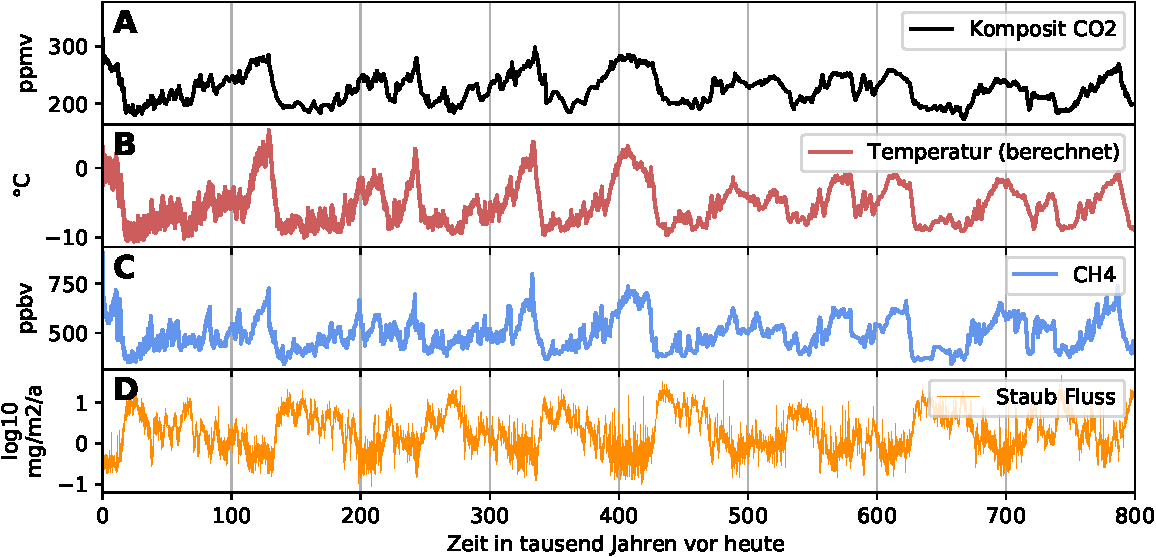
\includegraphics[width=\textwidth]{bilder/epica_icecore.pdf}
\caption{Zeitreihe der letzten 800 000 Jahre für die abgeleiteten Größen A) \cotwo, B) Temperatur, C) Methan (CH$_4$) und D) Staubkonzentrationen. Erstellt aus den Datensätzen des EPICA Dome C Eiskerns von \cite{Jouzel.2007}, \cite{Lambert.2012}, \cite{Loulergue.2008}, \cite{Bereiter.2015}, sh. Tabelle \ref{table:data}.}   \label{fig:icecore}
\end{figure}
Im ersten Schritt wird in Kapitel \ref{sec:Theorie} die relevante Theorie dargestellt und die Verbindung zwischen Staub, Phytoplankton und der Klimageschichte hergestellt. Im ersten Teil dieser theoretischen Basis wird in Kapitel \ref{sec:Eisenhypothese} die wegweisende Eisenhypothese \citep{Martin.1990} vorgestellt und die damit verbundene besondere Rolle des südlichen Ozeans erläutert. Um einen Einfluss von Staub oder Eisen auf Phytoplankton prüfen zu können, ist eine allgemeine Kenntnis des Phytoplanktons erforderlich, insbesondere der Prozesse, die zu einer Eisenlimitierung führen (Kapitel \ref{sec:Phytoplankton}). Im darauffolgenden Kapitel \ref{sec:Staub} werden wichtige Aspekte zu den Staubquellen in Australien vorgestellt, einer der Hauptspender des Elementes Eisen für den Ozean. Zum Abschluss des Kapitels wird schließlich noch der einzigartige Staubsturm \textit{Red Dawn} analysiert, welcher als Treiber der Phytoplankton-Reaktionen verdächtigt wird. Um diese Arbeit einzusortieren, wird außerdem ein Auszug an Ergebnissen von bisherigen vergleichbaren Arbeiten vorgestellt. In Kapitel \ref{sec:Methoden} werden anschließend die WRF-Simulation und die verwendeten statistischen Methoden präsentiert, mithilfe welcher der Staubsturm und dessen Auswirkungen genauer untersucht werden können. Das WRF-Modell bietet eine räumlich und zeitlich höhere Auflösung als bisherige Beobachtungsdaten und wurde speziell um ein Modul für Emission, Transport und Ablagerung von Staub erweitert. Der damit simulierte Staubeintrag in den benachbarten Ozean kann die chemische Zusammensetzung des Meerwassers entsprechend verändern und die Produktion von Phytoplankton fördern. Zur Bewertung dieser potentiellen Veränderungen wird die zeitliche Veränderung der Phytoplankton-Konzentrationen aus satellitengestützten Messungen des natürlichen Farbstoffs \textit{Chlorophyll a} abgeleitet. Basis für die Prüfung eines Zusammenhangs bilden Analysen der Zeitreihen, räumlichen Muster und letztlich verschiedene Korrelation- und Kovarianz-Tests. Daraufhin werden in Abschnitt \ref{sec:auswertung} die Ergebnisse der WRF-Simulation und die Auswertung der statistischen Methoden vorgestellt. Die Zeitreihenanalyse zeigt eine klare Reaktion, die sich von der gewöhnlichen Entwicklung und den Vorjahren abhebt. Die Interpretation der regionalen Muster ist jedoch schwieriger, es müssen weitere Annahmen getroffen werden. Zuletzt wird versucht, die Ergebnisse in \ref{sec:conclusion} einem Konzept zusammenzufassen, welches den Ablauf des Staubsturms und dessen Auswirkungen auf den Phytoplankton-Bestand chronologisch beschreibt.
\section{Theorie} \label{sec:Theorie}
Staub nimmt auf verschiedene Weise Einfluss auf das Klima. Der möglicherweise direkteste Einfluss wirkt auf die Energiebilanz. Staub ist mobil und kann unterschiedliche Strukturen und Formen annehmen. Durch die Ablagerung auf Oberflächen werden deren Reflektions- und Absorptionseigenschaften verändert. Während des Transports in der Atmosphäre kann Staub Strahlung auf noch komplexere Weise absorbieren, reflektieren, brechen, streuen oder emittieren \citep{Shao.2011} und somit die Temperaturverteilung beeinflussen. Einen deutlich indirekteren und verzögerten, aber nicht minder wichtigen Einfluss nimmt Staub auf den Kohlenstoffkreislauf, welcher wiederum wichtige Auswirkungen auf das Klima hat. Die Untersuchung im Rahmen dieser Arbeit betrifft genau diesen Einfluss, weshalb dieser im folgenden Kapitel beschrieben werden soll. In diesem Prozess sind mehrere Zwischenschritte enthalten, denen jeweils ein eigener Unterabschnitt gewidmet wird: Staub (Kapitel \ref{sec:Staub}) enthält Eisen, Eisen (Kapitel \ref{sec:Eisenhypothese}) reguliert Phytoplankton-Wachstum, Phytoplankton (Kapitel \ref{sec:Phytoplankton}) kontrolliert die \textit{Biologische Pumpe}, die Effektivität der biologischen Pumpe (\ref{sec:biopump}) nimmt Einfluss auf das Klima (\ref{sec:einleitung}).
\subsection{Der südliche Ozean und die Eisenhypothese} \label{sec:Eisenhypothese}
Der Region rund um die Antarktis wird ein mächtiger Einfluss auf das gesamte globale Klima zugerechnet. Einige Computermodelle können die regelmäßigen und \textit{globalen} Klimaveränderungen im derzeitigen Eiszeitalter ausschließlich mit Prozessen des südlichen Ozeans erklären \citep{Fischer.2010}. Klima und Wetter nördlich des antarktischen Kontinents werden stark durch den Zirkumpolarstrom \textit{(ACC, Antarctic Circumpolar Current)} beeinflusst. Der ACC umströmt die Landmasse zyklonal und ist gemessen an den Wassermassen die größte und für die globale Klimadynamik vermutlich wichtigste Meeresströmung überhaupt. Es wird davon ausgegangen, dass in dieser Region ein großer Teil der globalen Erwärmung umgesetzt wird. Schätzungsweise 45-62 \% der gesamten Wärmezunahme zwischen 2005 und 2017 in den oberen 2000m des globalen Ozeans entfielen auf den südlichen Ozean (IPCCpol.2019). Darüber hinaus sind die Ozeane verglichen mit der Atmosphäre wahre \cotwo -Speicher und nehmen einen Großteil (ca. 20-30 \%, vgl. \citep{IPCCpol.2019}) der anthropogenen \cotwo -Emissionen auf, wovon schätzungsweise etwa 40 \% auf diese Region entfallen \citep{Boning.2008}. Dies führt zu einer zunehmenden \textit{Versauerung} der Ozeane sodass der pH-Wert durch diese Entwicklung in diesem Jahrhundert weiter signifikant sinken wird \citep{IPCCpol.2019}. Der ACC verbindet Atlantik, Pazifik und den Indischen Ozean miteinander, was den Austausch von Wassermassen (und die globale thermohaline Zirkulation) überhaupt erst ermöglicht. Angesichts der enormen Relevanz dieser Region ist es wahrscheinlich, dass sämtliche Prozesse, die Einfluss auf ebendiese nehmen, auch Folgen für das globale Klima haben können.
\subsubsection{Zur Entwicklung der Eisenhypothese}
Grundsätzlich ist der südliche Ozean ein nährstoffreiches Gebiet und
bietet ein hohes Potential für die Produktion von Phytoplankton. Im Sommer sind große Teile der oberen Ozeanschichten ausreichend lichtdurchflutet und Nährstoffe können aus der Tiefe an die Oberfläche transportiert werden (Martin.1990). Der \textit{Ekman-Transport} befördert das durch die Reibung mit den \textit{Westerlies} (westlichen Winden) im ACC initial angetriebene Oberflächenwasser meridional nach Norden. Dieser Export wird südlich ausgeglichen, indem Tiefenwasser aufsteigt. Dieses an die Oberfläche beförderte Wasser ist i.d.R. nährstoffreicher als das Oberflächenwasser, da dessen Nährstoffe nicht permanent von der in der euphotischen Zone üppigeren Fauna konsumiert werden. Trotz dieses Nährstofftransports sind die dortigen Konzentrationen des Phytoplanktons im Mittel geringer, als man ursprünglich erwartet hatte. Die verfügbaren Nährstoffe werden nicht ausgeschöpft. Derartige Zonen mit hohem Nährstoffgehalt aber geringen Konzentrationen von Chlorophyll-haltigem Phytoplankton werden allgemein als HNLC (high nutrient low chlorophyll) Regionen bezeichnet. Es wurde bereits früh vermutet, dass unterschiedlicher Bedarf und Verfügbarkeit an Nährstoffen die Ursache für das gehemmte Wachstum ist. Der Nährstoffbedarf der Organismen ist sehr komplex und selbst heute sind noch nicht alle Zusammenhänge vollständig verstanden (sh. Kapitel \ref{sec:Phytoplankton}). Ein entscheidender Nährstoff ist Eisen. Spätestens nachdem Ende der 1980er im Nordosten des subarktischen Pazifiks gezeigt werden konnte, dass die künstliche \textit{Düngung} von Wasserproben mit Eisen zu einem deutlichen Anstieg der Phytoplankton-Produktion führen kann, war evident, dass Eisen ein wichtiger Nährstoff für Phytoplankton ist und das Wachstum limitieren kann \citep{Martin.1988}. Dieser Tatbestand war nicht überraschend, da praktisch alle lebenden Organismen Eisen benötigen. Bis dato war der Nachweis für Phytoplankton allerdings methodisch schwierig \citep{Martin.1988}. Insbesondere auf Basis dieses damals neuen Nachweises wird schließlich die Eisenhypothese formuliert.
\begin{figure}[htbp]
\centering
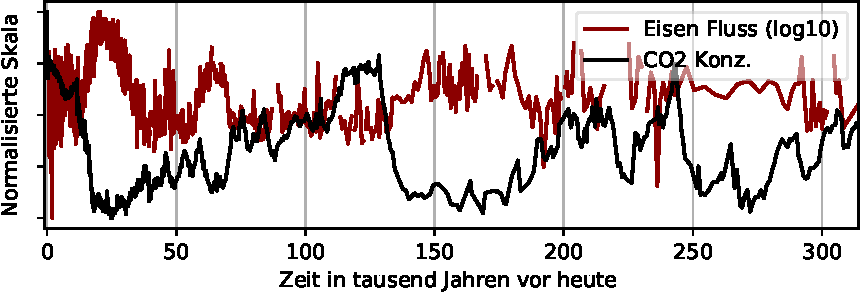
\includegraphics[width=0.8\textwidth]{bilder/co2_iron.pdf}
\caption{Zeitreihe der letzten 314 000 Jahre für die abgeleiteten Größen \cotwo \ (schwarz) und den Eisenfluss (dunkelrot), die zur Eisenhypothese inspirierte. Die Größen weisen insbesondere während der kälteren Glaziale eine starke Antikorrelation auf. Abnehmende \cotwo -Konzentrationen gehen mit erhöhtem Eisenfluss einher. Erstellt aus den Datensätzen von \cite{Bereiter.2015} und \cite{Vallelonga.2013}, sh. Tabelle \ref{table:data}.}   \label{fig:co2iron}
\end{figure}
Wie weiter oben beschrieben, übernimmt der südliche Ozean in der globalen Klimadynamik eine wichtige Rolle. Klimatische Änderungen in dieser Region korrelieren stark mit den natürlichen \cotwo -Konzentrationen der letzten 800 000 Jahre \citep{Fischer.2010}. Einfluss auf die \cotwo -Konzentrationen übt auch Phytoplankton aus, da im Rahmen der Fotosynthese \cotwo \ konsumiert, also der Atmosphäre / dem Ozean entzogen, und dabei in organische Kohlenstoffverbindungen (Glukose) und Sauerstoff umgesetzt wird. Während dieser \textit{Wachstumsphase} werden die umgebenden \cotwo -Konzentrationen durch den Konsum reduziert. Sorgen nun weitere Prozesse wie die \textit{Biologische Pumpe} (sh. Kapitel \ref{sec:biopump}) dafür, dass der auf diese Weise organisch gebundene Kohlenstoff dauerhaft von der Atmosphäre separiert wird, können die \cotwo \ Konzentrationen längerfristig reduziert werden. Potential für steigende Produktionsraten hat speziell der südliche Ozean als größte HNLC-Region. Könnten die überschüssigen Nährstoffe in großen Teilen dieser Region komplett durch Phytoplankton konsumiert werden, würde dies die globalen atmosphärischen \cotwo -Konzentrationen erheblich reduzieren \citep{Martin.1990}. Dass das nicht passiert, argumentiert \citet{Martin.1990} damit, dass das Wachstum von Phytoplankton im heutigen südlichen Ozean durch biologisch verfügbares Eisen limitiert ist. Ferner wird postuliert, dass ebendiese Limitierung für einen nennenswerten Anteil der in Abb. \ref{fig:icecore} beschriebenen Variationen der \cotwo -Konzentrationen zwischen Glazialen und Interglazialen verantwortlich ist, da sie sich im Laufe der Jahrtausende verändert. Der während der Glaziale höhere Staub- bzw. Eiseneintrag (sh. Abb. \ref{fig:co2iron}) soll höhere Menge an Eisen in den Ozean eingebracht und so die Produktion von Phytoplankton verstärkt haben. Die dadurch wiederum erhöhten \textit{Archivierungsraten} von organischem Kohlenstoff (sh. Kapitel \ref{sec:biopump}) hätten schließlich zu global reduzierten \cotwo -Konzentrationen geführt. Modelle berechnen, dass dies ungefähr die Hälfte des \cotwo \ Rückgangs bei Einsetzen der Glaziale erklären könnte. Für die Eisenhypothese ist entscheidend, dass Eisen in küstenfernen Gebieten hauptsächlich durch äolischen Staub eingebracht wird. Der Großteil der Hauptnährstoffe wird hingegen durch Flüsse in den Ozean eingetragen, welche die Produkte der Verwitterung von den Landmassen abtransportieren \citep{Emerson.2009}. Staubquellen sind in der südlichen Hemisphäre deutlich weniger ausgeprägt als auf der Nordhalbkugel \citep{Shao.2011}. Darüber hinaus kann Staub neben einem \textit{düngenden} Effekt auch direkten Einfluss auf den Kohlenstofffluss in Richtung Tiefsee nehmen, indem Staubpartikel mit organischem Material im Oberflächenwasser aggregieren und die Sinkgeschwindigkeit damit erhöhen \citep{vanderJagt.2018}.
\subsubsection{Die Eisenhypothese heute}
Die Eisenhypothese wurde inzwischen in mehreren Experimenten getestet. Es konnte tatsächlich gezeigt werden, dass die Zufuhr von Eisen die Produktion in entsprechenden Regionen mit geringen Chlorophyll-Konzentrationen steigern kann \citep{Boyd.2007}. Im SOIREE (Southern Ocean Iron Release Experiment) wurden Reaktionen auf die Eisendüngung nach etwa 5 Tagen beobachtet. Hauptsächlich wurde das Wachstum größerer Kieselalgen gefördert \citep{Trull.2001}. Es konnte allerdings nicht gezeigt werden, dass zusätzlich der Export durch die \textit{Biologische Pumpe} erhöht wurde. In vielen Regionen des südlichen Ozeans scheint dieser Export zusätzlich durch die Verfügbarkeit von Silizium limitiert. Die sogenannte \textit{Silizium-Pumpe} (beschleunigtes Absinken des Phytoplanktons durch erhöhte Dichte aufgrund der Siliziumdioxid-Frusteln, vgl. Abschnitt \ref{sec:biopump}) arbeitet bereits am Limit, hohe Silikat-Konzentrationen beschränken sich auf den Süden (sh. Abb. \ref{fig:factors_collage}). Während geschätzt wird, dass bei etwa 40 \% des ozeanischen Oberflächenwassers Eisen ein limitierender Faktor für die Produktion von Phytoplankton sein kann \citep{Emerson.2009}, wird der Beitrag des durch äolischen Staub eingetragenen Eisens auf den Kohlenstoffkreislauf inzwischen geringer eingeschätzt. \citet{Tagliabue.2017} fassen zusammen, dass auch weitere Prozesse für die Verteilung des biologisch verfügbaren Eisens (sh. Kapitel \ref{sec:Phytoplankton}) im Ozean anerkannt sind und besonders in geographisch höheren Breiten gegenüber dem Staubeintrag dominieren können. \citet{Vallelonga.2013} schätzen den (Staub-)Beitrag zur Variabilität nach dem letzten glazialen Maximum (LGM) auf maximal 20 ppmv \cotwo . Es wird angenommen, dass die (inter)glazialen \cotwo -Schwankungen durch eine Kombination aus \textit{Eisendüngung}, Veränderungen bei den Karbonatkompensationen (Auflösung von Calcit und Aragonit mit  \cotwo \ zu Calcium und Bikarbonat in der Tiefsee) und Ventilation des südlichen Ozeans \citep{Lambert.2012} gesteuert werden. Die Analyse der Phasenverschiebung zwischen Staubflüssen und \cotwo -Konzentrationen von \citet{Lambert.2012} zeigt, dass die Eisendüngung des südlichen Ozeans durch Staub jedenfalls gegen \textit{Ende} der letzten 9 Glaziale offenbar nicht der dominante Faktor für den Anstieg der \cotwo -Konzentrationen war. Der Staubfluss erreicht stets etwa 4.000 Jahre früher die für Interglaziale typischerweise  geringen Werte, während sich \cotwo \ und Temperatur noch verändern (ansteigen) können. Offen bleibt, wie hoch der Beitrag tatsächlich ist und ob ggf. umgekehrt die Eisendüngung zu \textit{Beginn} der Glaziale dennoch ein dominanter Faktor zur \textit{Reduzierung} der Konzentrationen sein kann. \citet{MartinezGarcia.2009} folgern hierzu anhand des zeitlichen Eintretens der Effekte allerdings ebenfalls, dass der ursächliche Anstoß des starken Abfalls der \cotwo -Konzentrationen eher durch physikalische Prozesse erfolgte, wie Veränderungen der antarktischen Meereisausdehnung, Stratifizierung des Oberflächenwassers und die geographische Ausdehnung der sogenannten \textit{Westerlies}. Dennoch wird der Eisendüngung weiterhin ein substantieller Anteil zugeschrieben. Lässt sich (wie im Rahmen dieser Arbeit untersucht) zeigen, dass die vergleichsweise (ggü. nördl. Hemisphäre) seltenen Staubereignisse einen signifikanten Einfluss auf die Phytoplankton-Produktion nehmen, wäre dies in diesem Zusammenhang ein wichtiger Mechanismus und Indiz für eine höhere Relevanz des äolischen Staubs.
\subsection{Eigenschaften und Abhängigkeiten von Phytoplankton} \label{sec:Phytoplankton}
Phytoplankton ist das wichtigste Bindeglied in der hier beschriebenen Wirkungskette. Es konsumiert das potentiell durch einen Staubsturm zur Verfügung gestellte Eisen, bindet \cotwo \ und kann dieses durch Absinken für lange Zeit von der Atmosphäre separieren. In diesem Kapitel wird kurz erläutert, in welcher Form Phytoplankton Eisen konsumiert, und 
welche weiteren Besonderheiten aufgrund der Region, in dem es wächst, zu berücksichtigen sind. Beide Aspekte müssen in der späteren Auswertung zur Interpretation berücksichtigt werden.
\subsubsection{Allgemeines zu Phytoplankton} \label{sec:Phytobasics}
Durchschnittlich ca. 10 µg pro Liter bzw. $10^{-6}$ Prozent des Oberflächenwassers bestehen aus lebenden Organismen \citep{Emerson.2009}. Obwohl die Konzentration an Land weitaus größer ist, nehmen Kleinstorganismen wie Phytoplankton einen erheblichen Einfluss auf ihre Umwelt. Neben dem regulierenden Einfluss auf die Atmosphäre (sh. Kapitel \ref{sec:Eisenhypothese}) bilden diese einzelligen und \textit{autotrophen} (sich nur von Sonnenlicht \textit{ernährenden}) Lebewesen die Basis der Nahrungskette. Die Lebenserwartung von Phytoplankton beträgt lediglich Stunden bis hin zu Tagen, wodurch es praktisch ausschließlich Eigenschaften des umgebenden Ozeanwassers annimmt. Neben der Abhängigkeit von der Verfügbarkeit der notwendigen Nährstoffe werden Bestand und Wachstum durch das in der Nahrungskette nächsthöhere Zooplankton reguliert, welches sich von Phytoplankton ernährt. \citet{Boyce.2010} folgern, dass der Reichtum an Phytoplankton insgesamt seit Beginn der Messungen (1899) aufgrund der Erwärmung der Ozeane abgenommen hat und dass das globale Median jährlich um etwa 1\% abnimmt. Da die Klimamodelle steigende (Meeres-)Temperaturen prognostizieren, ist es wahrscheinlich und problematisch, dass die Menge an Phytoplankton (der Basis aller Nahrungsketten im Ozean) zukünftig noch weiter abnimmt \citep{Siegel.2010}. Klimaänderungen werden außerdem direkt (aufgrund veränderter Ozeanchemie) und indirekt (Änderungen in der Ozeanzirkulation) die Verteilung des Phytoplanktons verändern \citep{Falkowski.1998}. Je nach Region und Jahreszeit wird das Ozeanwasser durch verschiedene Unterarten des Phytoplanktons repräsentiert. Die das Picophytoplankton ($<2\mu$m) in vielen Teilen des Ozeans dominierenden Cyanobakterien \textit{Synechococcus} und \textit{Prochlorococcus} enthalten vermutlich am meisten der grünen, Licht absorbierenden Pigmente (Chlorophyll) \citep{Emerson.2009}. \textit{Kieselalgen} dominieren in Regionen, in denen aufsteigendes Wasser nennenswerten Einfluss nimmt, wie bspw. im südlichen Ozean, siehe Abbildung \ref{fig:dominant_diatom_pico}. Dort besteht das Sediment größtenteils aus den \textit{Frusteln} (Schalen, die überwiegend aus Siliziumdioxid SiO$_2$ bestehen) der Kieselalgen. Für Kieselalgen ist die Zufuhr von Kieselsäure daher essenziell und wachstums-limitierend; diese tritt fast ausschließlich südlich der Südpolarfront auf \citep{Falkowski.1998}, sh. auch Abb. \ref{fig:factors_collage}. Eine mögliche Limitierung durch Silizium spielt insbesondere im  hier später näher untersuchten Tasmanischen Meer eine Rolle. Dort kann Silikat durch entsprechende Strömungen aus dem südlichen Ozean advehiert werden.
\begin{figure}[htbp]
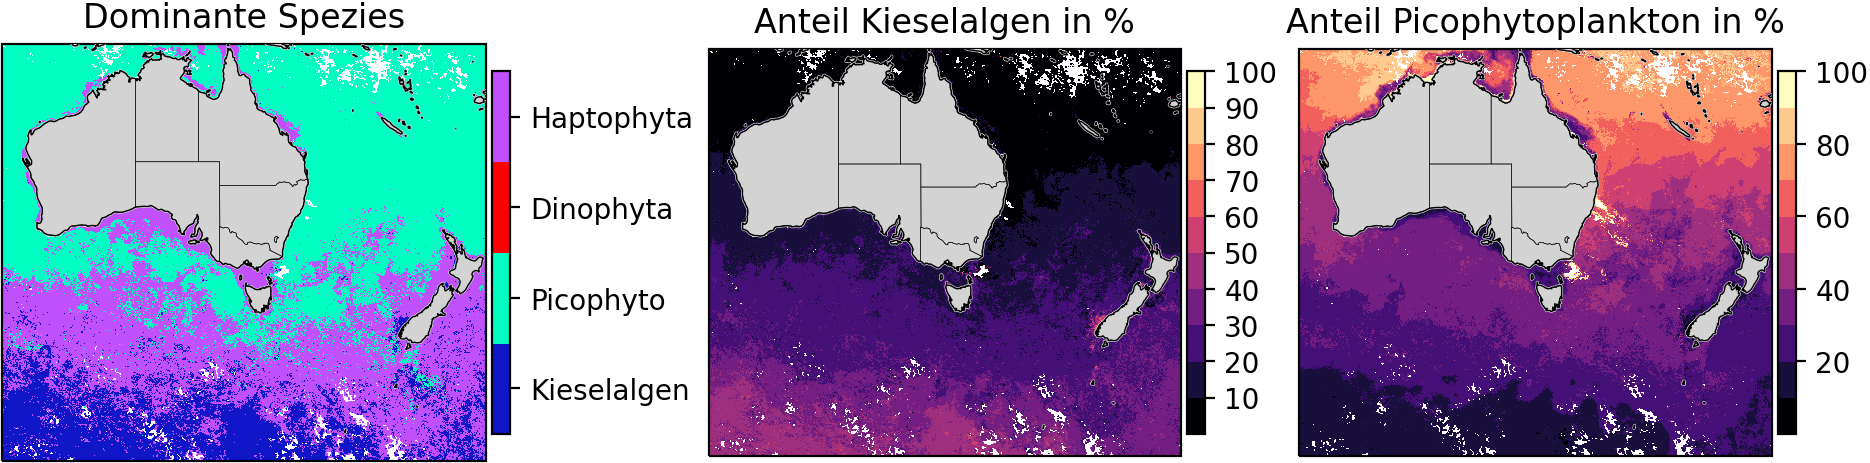
\includegraphics[width=\textwidth]{bilder/dominant_diatom_pico.png}
\caption{Übersicht der dominanten Phytoplankton-Spezies im Untersuchungsgebiet für den Monat Oktober 2009. Die Konzentrationen wurden aus Satellitengestützten Messungen abgeleitet, für weitere Informationen siehe Tabelle \ref{table:data}}. \label{fig:dominant_diatom_pico}
\end{figure}
\subsubsection{Nährstoffe} \label{sec:nährstoffe}
Auch autotrophe Organismen benötigen zur Entwicklung neben dem einfallenden Sonnenlicht weitere Nährstoffe, aus denen sie sich später zusammensetzen. Diese werden in Makro- und Mikronährstoffe kategorisiert. Die Makronährstoffe Kohlenstoff (C), Stickstoff (N) und Phosphor (P) sind artenübergreifend  Hauptbestandteile des Phytoplanktons. Diese werden ungefähr im Verhältnis (106C/16N/1P) konsumiert \citep{Falkowski.1998}. Eine abgeleitete näherungsweise, nicht allgemeingültige Formel für die Fotosynthese  \citep{Emerson.2009} veranschaulicht die chemische Zusammensetzung und den Bedarf an den Hauptnährstoffen C, N und P:
\begin{equation}
\text{106\cotwo} + \text{16HNO}_3 + \text{H}_3\text{PO}_4 + \text{122H}_2\text{O} \rightarrow \text{(CH}_2\text{O)}_{106}\text{(NH}_3\text{)}_{16}\text{H}_3\text{PO}_4 + \text{138O}_2
\end{equation}
Neben diesen relativ gut bekannten Abhängigkeiten von den Makronährstoffen sind die in viel geringerer Menge notwendigen (und verfügbaren) Mikronährstoffe aber genauso wichtig und können das Wachstum limitieren, wenn sie fehlen. Zu diesen Mikronährstoffen gehören beispielsweise Spurenelemente wie Mangan, Eisen, Kobalt, Nickel, Kupfer und Zink. Ein Teil dieser Metalle wird durch (mutmaßlich aus biologischen Prozessen entstandenen) Liganden besetzt/komplexifiziert, was die biologische Verfügbarkeit für das Phytoplankton einschränken kann. Die Natur dieser Liganden ist noch nicht vollumfänglich verstanden. Allerdings wird davon ausgegangen, dass ausschließlich die weiterhin \textit{freien} Metalle biologisch verfügbar sind \citep{Emerson.2009}, d.h. von Phytoplankton konsumiert werden können. Demgegenüber können sich Liganden auch positiv auf Eisenkonzentrationen auswirken, indem das Eisen durch die Besetzung in gelöster Form verbleibt, also nicht absinkt/aggregiert, und über größere Strecken transportiert werden kann \citep{Tagliabue.2017}. Berücksichtigt man diese weiteren Mikronährstoffe, lässt sich wieder ein stöchiometrisches Verhältnis (Gl. \ref{eq:stochio}) ableiten, das an dieser Stelle weiter nicht exakt oder allgemein gilt, sondern nur die Größenordnungen der Beiträge exemplarisch aufzeigen soll \citep{Emerson.2009}. Insbesondere der Bedarf an Eisen kann je nach Umgebung höchst unterschiedlich sein.
\begin{equation}
\text{(C}_{106} \text{N}_{16} \text{P)}_{1000} \text{Fe}_8\text{Mn}_4\text{Zn}_{0.8}\text{Cu}_{0.4}\text{Co}_{0.2} \text{Cd}_{0.2} \label{eq:stochio}
\end{equation}
Es wurde beobachtet, dass die Entwicklung des Phytoplanktons von allen Nährstoffen entsprechend \textit{Liebig's Law} abhängt. Demnach ist das Wachstum durch den Nährstoff beschränkt, der im geforderten Verhältnis am wenigsten verfügbar ist. Dadurch bilden sich die bereits in Kapitel \ref{sec:Eisenhypothese} HNLC-Regionen, in denen zwar viele Nährstoffe im Überfluss vorhanden sind, jedoch nicht konsumiert werden können, weil ein Baustein fehlt. Diese Beobachtung ist für die Eisenhypothese wesentlich, wonach der Nährstoff Eisen für den Großteil dieser ungenutzten Potentiale verantwortlich sein soll. \citet{Martin.1988} zeigten zunächst exemplarisch für eine Region in isolierten Behältern, dass die übrigen Nährstoffe nach Zugabe von Eisen etwa 4 Tage später tatsächlich konsumiert wurden. Aufgrund des Konsums durch Phytoplankton sind Eisen und andere Nährstoffe an der Ozeanoberfläche häufig im Vergleich zu tieferen Schichten (in welchen das licht-abhängige Phytoplankton nicht überlebt) reduziert \citep{Martin.1990}. Die Konzentrationen des Elements Eisen im Meerwasser sind verglichen mit den häufigsten Stoffen wie Natrium, Chlorid, Sulfat und Magnesium sehr gering. Dennoch ist es das dritthäufigste Element in marinen Sedimenten \citep{Emerson.2009}. Wie lange Eisen in den oberen Schichten verbleibt, hängt vordergründig vom chemischen Zustand ab. In gelöster Form sinkt Eisen kaum und kann etwa 6 Monate in Tiefen bis max. 150m residieren \citep{Hayes.2015}. In Form von Aggregaten und größeren Partikeln ist die Sinkgeschwindigkeit jedoch deutlich höher. In einer Fallstudie für einen vorangegangenen Staubsturm gehen \citet{Boyd.2010} von einer Verweilzeit in oberflächennahen Schichten von 30 Tagen für äolisch eingebrachtes Eisen aus. Eisen tritt häufig in einer nicht biologisch verfügbaren Form auf. Insbesondere innerhalb von Staub kommt Eisen in der kaum löslichen Form Fe$^\text{3+}$ anstatt des gut löslichen Fe$^\text{2+}$ vor \citep{Reynolds.2014}. Im südlichen Ozean kann auch Mangan ein limitierender Nährstoff sein \citep{Browning.2021}. Bisher wurde Mangan diesbezüglich nicht verdächtigt. Die Besonderheit bei Mangan ist, dass dieses Spurenmetall im Gegensatz zu Eisen kaum durch Liganden besetzt wird und damit biologisch verfügbarer ist \citep{Emerson.2009}. In Abbildung \ref{fig:factors_collage} sind einige wichtige Parameter und die Nährstoffverteilung des Meerwassers für die im Rahmen dieser Arbeit untersuchte Region im September 2009 dargestellt. Bei allen Darstellungen sind deutliche Änderungen mit der geographischen Breite mit einer relativ scharfen Grenze auf Höhe der südlichen Grenze des australischen Kontinentes zu erkennen. Das Tasmanische Meer enthält offensichtlich Merkmale sowohl der nördlichen als auch der südlichen Region und beschreibt einen Übergang zwischen diesen. Die wichtigen Nährstoffe Nitrat und Phosphat (Abb. \ref{fig:factors_collage} A, B) sind in dem als HNLC-Region deklarierten südlichen Ozean deutlich erhöht und werden im Tasmanischen Meer mit vergleichsweise hohen durchschnittlichen Chlorophyll-a-Konzentrationen und Primärproduktionen (sh. I) reduziert. In C) wird deutlich, dass sich die für Kieselalgenblüten wichtigen, hohen Silikat-Konzentrationen deutlich auf die südlicheren Regionen beschränken.
\begin{figure}[htbp]
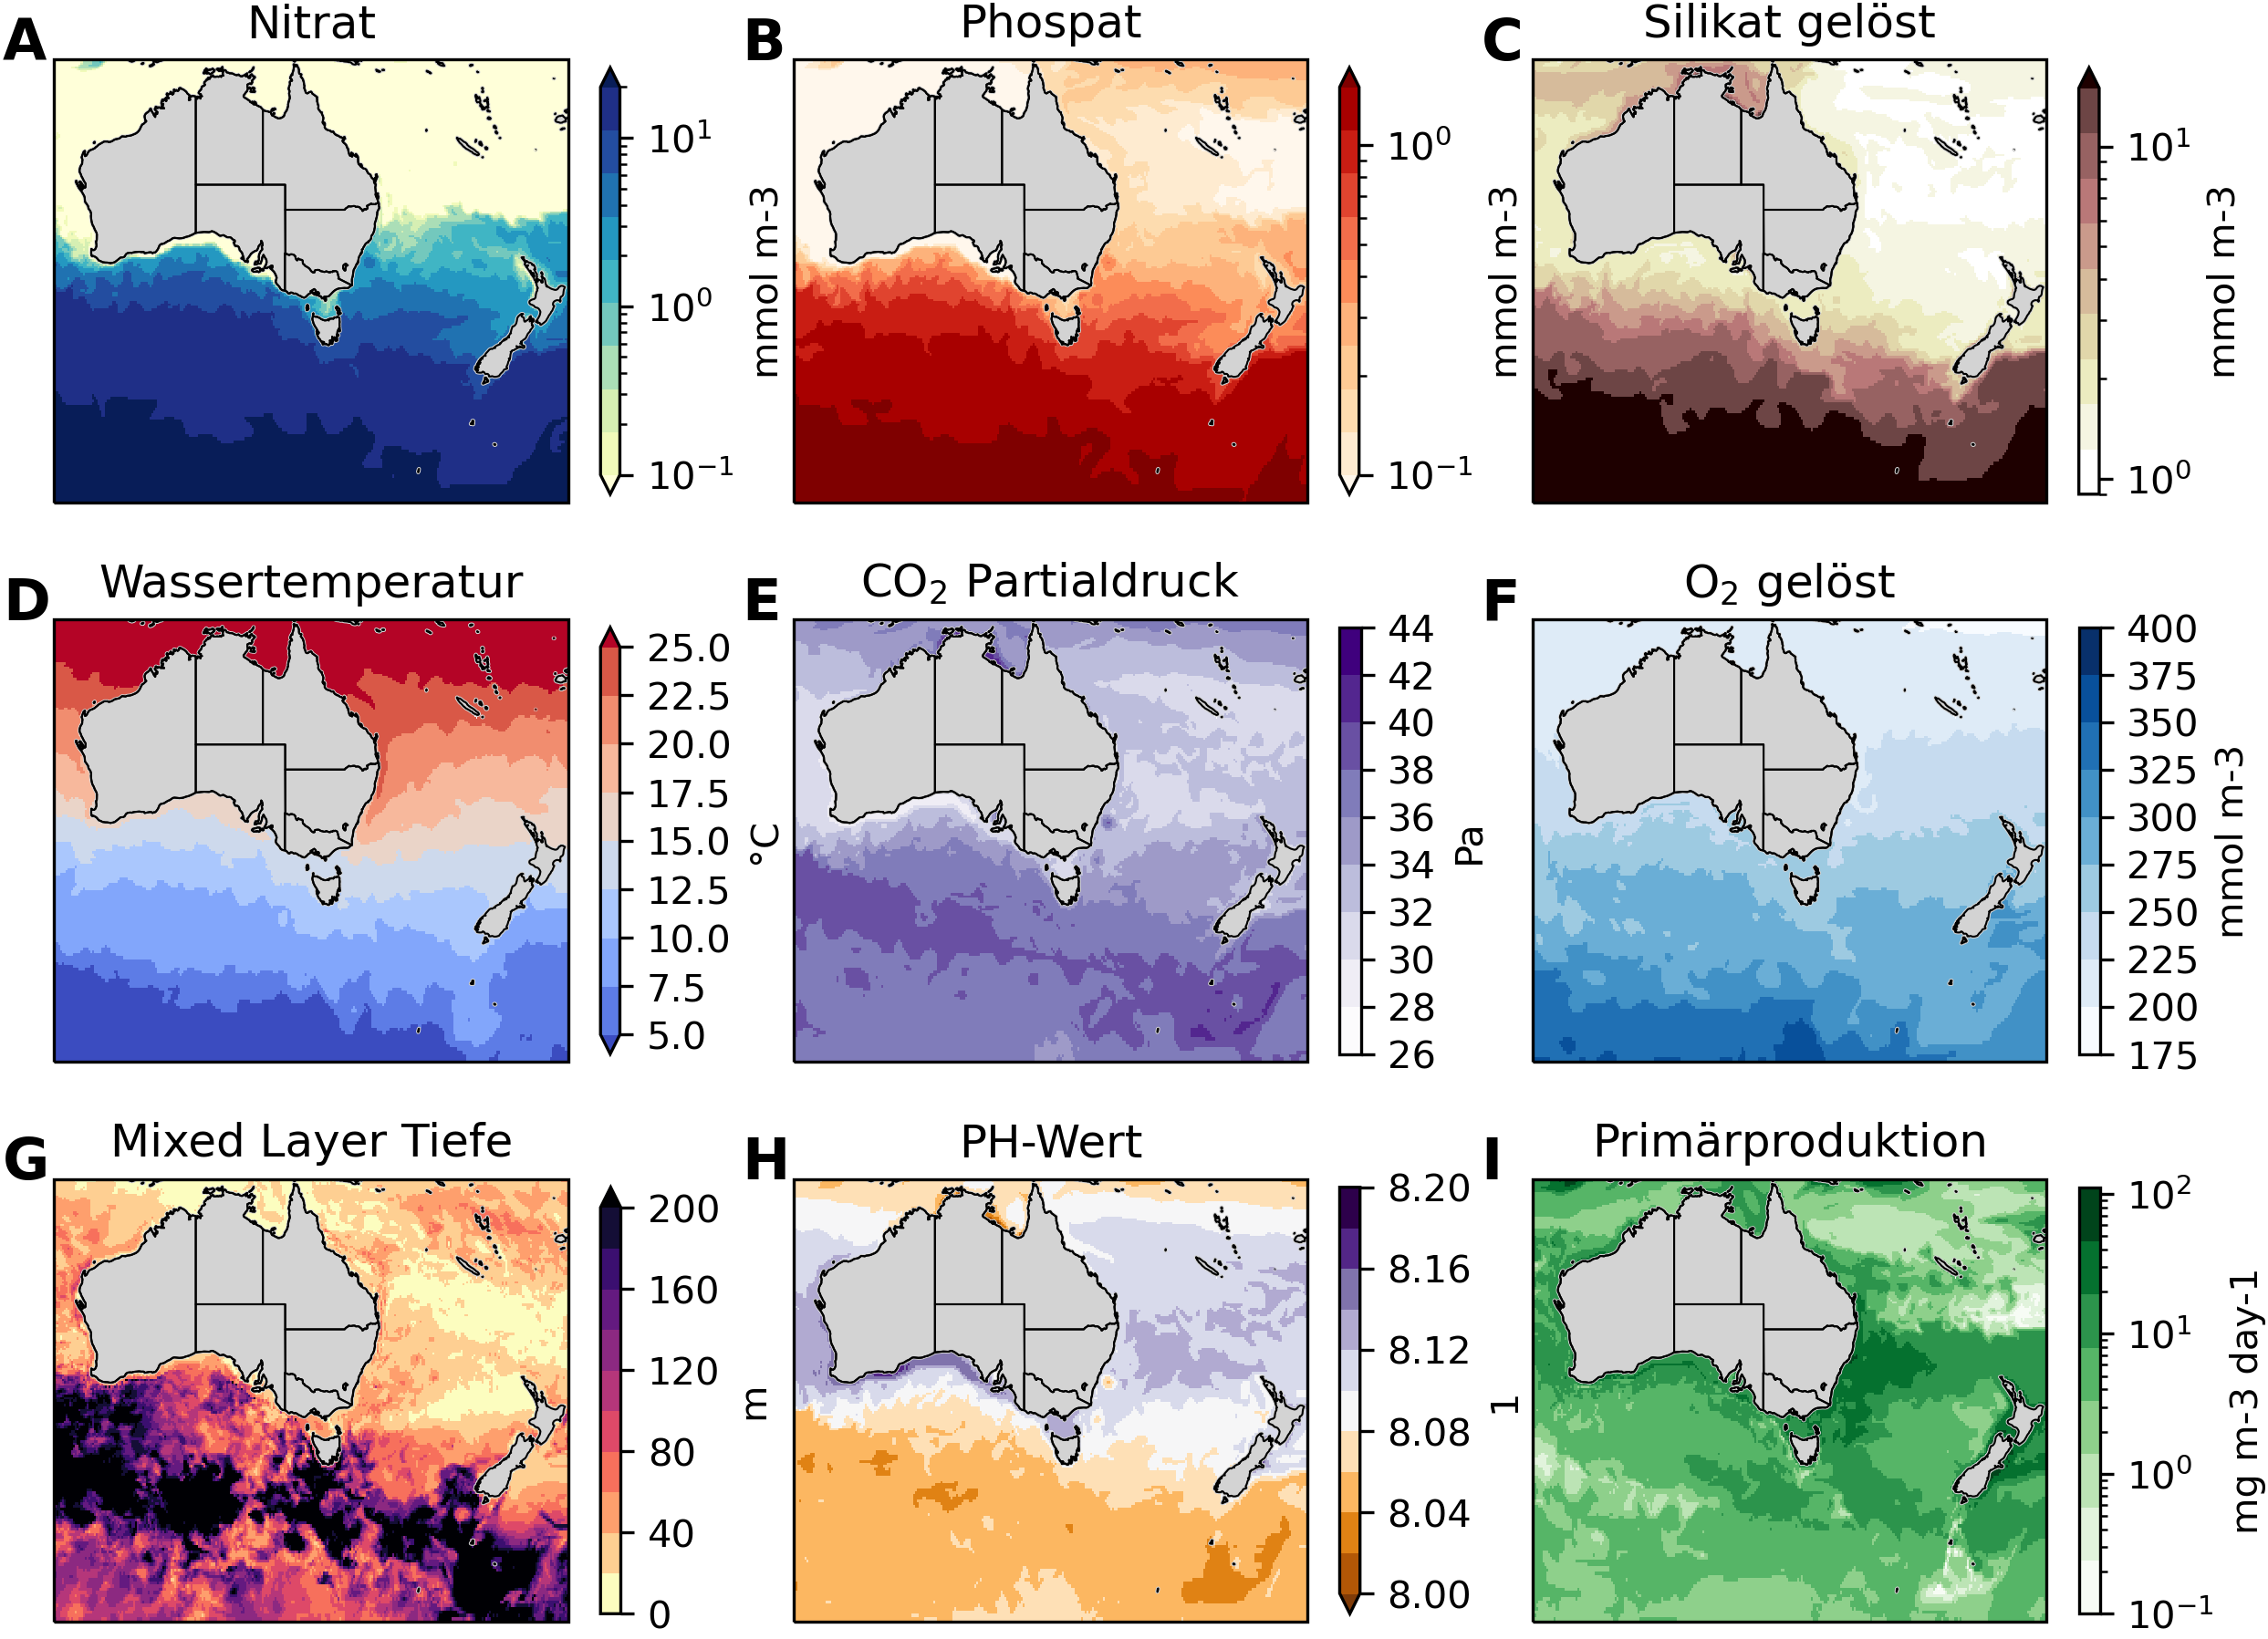
\includegraphics[width=\textwidth]{bilder/factors_collage.png}
\caption{Eine Zusammenstellung wichtiger Ozean-Parameter. Monatliche Daten des  Marine Copernicus Service, sh. Tabelle \ref{table:data}}. \label{fig:factors_collage}
\end{figure}
Neben dem direkten Einfluss als Nährstoff kann Eisen das Wachstum von Phytoplankton noch in Form von Enzymkomplexen fördern. Das Enzym \textit{Nitrogenase} kann N$_2$ reduzieren und Stickstoff biologisch verfügbar machen. Dieser Prozess ist in Regionen entscheidend, in denen das Wachstum hauptsächlich durch mangelnde biologische Verfügbarkeit von Nitraten beschränkt ist. Diese werden \textit{low nitrate low chlorophyll} (LNLC) Regionen genannt und können ebenso wie die HNLC-Gebiete durch zusätzliches Eisen erhöhte Wachstumsraten aufweisen. Wie man auf Abbildung \ref{fig:factors_collage} sehen kann, trifft dies auf die dort gezeigten tropischen Gewässern zu. Die Zugabe von Eisen fördert außerdem, dass Nitrate (NO$_3^-$) zu Ammonium-Ionen (NH$_4^+$) reduziert werden, welche bei der Fotosynthese von Plankton mit hohem Bedarf an Nitraten besonders schnell verwendet werden können \citep{Emerson.2009}. Laut \citet{Emerson.2009} ist dies sogar das extremste Beispiel für die Limitierung durch Eisen, da die Enzyme zu einem substanziellen Teil aus Eisen bestehen. Diese Funktion wurde insbesondere bei der diazotrophen Phytoplankton-Art \textit{Trichodesmium} beobachtet \citep{Falkowski.1998}. In nährstoffarmen LNLC-Gewässern haben derartige extrem kleine Phytoplankton-Organismen bei der Verarbeitung von Nährstoffen (Exkrementen der Verbraucher) aufgrund des größeren Oberflächen- zu Volumen- Verhältnisse einen Wettbewerbsvorteil \citep{Falkowski.1998}. Wenn hingegen \textit{neue} Nährstoffe bspw. durch Aufströmen in das lichtdurchflutete Oberflächenwasser gelangen, hat größeres Phytoplankton, insbesondere Kieselalgen, einen Wettbewerbsvorteil (aufgrund Vakuole, schnellere Nährstoffaufnahme). Entsprechende Phytoplankton-\textit{Blüten} bestehen dadurch häufig aus Kieselalgen \citep{Boyd.2007}, wenn das Nährstoffangebot plötzlich erhöht ist. Das Plankton, das sich wiederum von diesen ernährt und den Bestand damit reguliert, ist typischerweise größer, benötigt für Entwicklung (Larvenstadium) mehr Zeit, wodurch Blüten überhaupt erst möglich sind. Die Biologische Pumpe (Kapitel \ref{sec:biopump}) kann als Folge derartiger Blüten intensiviert werden. 
\subsubsection{Biologische Pumpe} \label{sec:biopump}
Das Ökosystem innerhalb der euphotischen Zone arbeitet sehr effizient. Die im Phytoplankton enthaltenen Nährstoffe werden nach dem Absterben oder \textit{Abgrasen} durch Zooplankton sehr schnell wieder remineralisiert und für die nächste Generation in der Nahrungskette verwendet. Entsprechend wenig Material entkommt den oberflächennahen Schichten, bevor es wieder konsumiert wird. Durch temporär erhöhte Phytoplankton-Konzentrationen alleine erfolgt noch keine dauerhafte Archivierung des Kohlenstoffs, obwohl dieses zunächst bei der Photosynthese in organischem Material gebunden wurde. Nur wenn dieses bis auf den Meeresgrund sinkt, ist es dem Kreislauf der Wiederfreisetzung für bis zu Jahrtausende entzogen. Dieser Prozess des Absinkens organischen Kohlenstoffs wird \textit{Biologische Pumpe} genannt. Der Export von organischer Materie aus der euphotischen Zone ist für den Hauptteil der chemischen Prozesse in der Tiefsee verantwortlich \citep{Emerson.2009}. Ein niedriger Sauerstoffgehalt in der Tiefsee weist auf eine starke Biologische Pumpe hin. Der sinkende organische Kohlenstoff wird zersetzt, wodurch \cotwo \ freigesetzt und Sauerstoff konsumiert wird (umgekehrte Fotosynthese, \cite{Honjo.2008}). Im aktuellen Ozean beträgt der durchschnittliche (Sink-)Fluss zwischen dem Meso- und Bathypelagial in etwa 2 km Tiefe ca. 0.84 Pg Kohlenstoff (organisch+anorganisch) pro Jahr \citep{Honjo.2008}. Aufgrund der höheren Dichte von Mineralen (vereinfachend angenommen ca. $2.5$ g/cm$^{-3}$) im Gegensatz zu organischer Materie (ca. $1.1$ g/cm$^{-3}$) und Meerwasser (ca. $1$ g cm$^{-3}$) kann abgeschätzt werden, dass anorganische Partikel etwa 15 mal schneller sinken als rein organische. Folglich kann abgeleitet werden, dass Organismen ohne zusätzlichen mineralischen Ballast aufgrund der geringen Sinkgeschwindigkeit die euphotische Zone praktisch kaum verlassen können. Zusätzlich bietet eine mineralische Hülle entsprechenden Schutz vor Oxidation der organischen Materie, die ansonsten bereits innerhalb der ersten 2 000m während des Sinkens einsetzen würde \citep{Emerson.2009}. Demzufolge können Blüten derjenigen Unterarten des Phytoplanktons, wie Kieselalgen und Coccolithoporida, die sogenannte Frusteln aus Siliziumdioxid respektive Kalziumkarbonat bilden, die Biologische Pumpe temporär beschleunigen. Es wird angenommen, dass die Leistung der Biologischen Pumpe (d.h. der Sinkfluss) aufgrund der Klimaveränderungen insgesamt global abnehmen wird. Auch der wichtige Nährstoff Eisen wird im Rahmen der Biologischen Pumpe recycelt und teilweise in die Tiefsee befördert. Da die Remineralisierung (das \textit{Verfügbarmachen}) länger dauern kann als bei anderen Elementen, wird Eisen diesem Kreislauf tendenziell schneller wieder entzogen. Darüber hinaus führt hoher Sauerstoffgehalt zu einer schnellen Oxidation des Eisens, welches dadurch kaum noch löslich ist und sinkt \citep{Falkowski.1998}. Diese  Effekte tragen zur Eisenarmut des Oberflächenwassers vieler Regionen bei.
\subsubsection{Meeresströmungen und Mixed Layer}
Wie in den vorangegangenen Kapiteln beschrieben, hängt die Entwicklung des Phytoplanktons neben der zur Fotosynthese unverzichtbaren Sonne von der Verfügbarkeit der Nährstoffe ab. Diese Verfügbarkeit wird wiederum durch Meeresströmungen gesteuert. Die Mischschicht des Oberflächenwassers (englisch \textit{Mixed Layer}) bezeichnet die Zone des Oberflächenwassers, in welcher die Bestandteile (d.h. auch das Phytoplankton) des Ozeanwassers größtenteils homogen durchmischt werden. Die Veränderung der Tiefe dieser Mischschicht (MLD, \textit{Mixed Layer Depth}) kann sowohl positive als auch negative Auswirkungen auf die Entwicklung des Phytoplanktons haben: Durch eine Vertiefung werden weitere Meeresschichten, deren Nährstoffe bisher weniger konsumiert wurden, einbezogen, sodass sich der durchschnittliche Nährstoffgehalt erhöhen kann. Gleichzeitig erreicht den tieferen Teil der Mischschicht weniger Sonnenlicht, sodass dies ein limitierender Faktor für die Entwicklung des Phytoplanktons sein kann. Ein Abflachen der MLD geht häufig mit erhöhter Sonneneinstrahlung einher, welche das Oberflächenwasser thermodynamisch stabilisiert und stratifiziert. Dann steht zwar mehr Sonnenlicht zur Verfügung, die Nährstoffe werden aber (bis zur Limitierung durch den am wenigsten verfügbaren Nährstoff) schneller aufgebraucht. Aufgrund der jahreszeitlich variierenden Sonneneinstrahlung folgt die MLD vielerorts einem jahreszeitlichen Gang. Im südlichen Ozean beträgt die MLD häufig mehrere hundert Meter, kann im Sommer aber auf durchschnittlich weniger als 50m Tiefe abflachen (vgl. Abbildung \ref{fig:mld_currents}). Die zunehmende Sonneneinstrahlung mit Einsetzen des Frühlings im September führt zwangsläufig zu einer deutlich reduzierten MLD. Im Tasmanischen Meer fördert dieser Trend Phytoplankton-Blüten im Frühling \citep{Tilburg.2002}. Neben der MLD können dort Wirbel (\textit{Eddies}) einen erheblichen Einfluss nehmen. Aufgrund der Corioliskraft bzw. des Ekman-Transports wird das Oberflächenwasser in zyklonalen Strömungen radial nach außen abtransportiert, sodass kälteres, nährstoffreicheres Wasser aus größeren Tiefen aufströmt. Während dieser Nährstofftransport die Entwicklung des Phytoplankton innerhalb zyklonaler Wirbel fördert, führt umgekehrt die erhöhte Stratifizierung durch Kumulierung der Wassermassen im Kern antizyklonaler, dadurch wärmerer, Wirbel zu einer Dämpfung des Wachstums. In Regionen wie dem Tasmanischen Meer, in welchem aufgrund des östlich abgelenkten Ostaustralstroms (EAC, \textit{East Australian Current} besonders ausgeprägte Wirbel entstehen, können diese Effekte zu einem sehr heterogenen Muster der Phytoplankton-Konzentrationen führen \citep{Tilburg.2002}. Wie auf Abbildung \ref{fig:mld_currents} sichtbar, scheint der Verlauf der Stromlinien das Muster der Chlorophyll-a Konzentrationen zu bestimmen. Im Kern antizyklonaler Wirbel entwickelt das Phytoplankton eher schwach, entsprechend gering sind häufig die Konzentrationen. In zyklonalen Wirbel zeigt sich eine gegenteilige Entwicklung.
\begin{figure}[htbp]
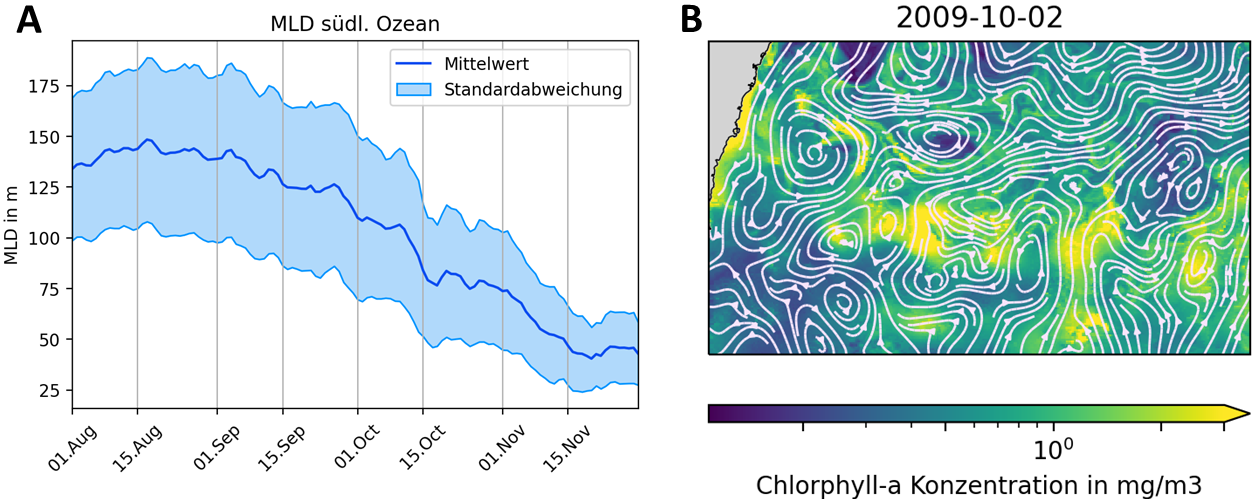
\includegraphics[width=\textwidth]{bilder/mld_currents.png}
\caption{A) Mittlere MLD für einen Teil (40°E-80°W, 32°S-65°S) des südlicheren Ozeans für den Zeitraum August bis Dezember 2009. B) Beispielhafte Chlorophyll-a Konzentrationen und Stromlinien des Oberflächenwassers im Tasmanischen Meer für den 2. Oktober 2009. Chlorophyll-a Daten sh. Kapitel \ref{sec:chla}, Strömungs- und MLD-Daten sh. Tabelle \ref{table:data}.} \label{fig:mld_currents}
\end{figure}
\subsection{Staub in Australien} \label{sec:Staub}
Die südliche Hemisphäre hat wegen der wenigen Landmassen weniger Staubquellen, wodurch die Atmosphäre in Umgebung des antarktischen Zirkumpolarstroms vergleichsweise staubarm ist. Die größte Staubquelle bietet die hier untersuchte Region Australien \citep{Shao.2011}. In diesem Kapitel sollen die Regionen mit den höchsten Emissionspotentialen präsentiert werden (Kapitel \ref{sec:staubquellen}), um deren Einfluss bei der späteren Simulation bewerten zu können. Darüber hinaus wird auf den wichtigen Nährstoff Eisen und dessen Vorkommen in Staub eingegangen. Anschließend wird das besondere Staubereignis, das sogenannte \textit{Red Dawn Event} vorgestellt.
\subsubsection{Staub- und Eisenquellen} \label{sec:staubquellen}
Die Haupt-Staubquelle erstreckt sich über ein riesiges Gebiet in Zentralaustralien \citep{Shao.2011}. Das sogenannte Lake Eyre Becken liegt im Zentrum eines endorheischen Systems. Dieses System führt dazu, dass die Bestandteile emittierten Staubs anderen Regionen entstammen können und über weite Strecken transportiert wurden. Diese Ursprünge sind i.d.R. benachbarte Regionen höherer Feuchte, in denen chemische und physikalische Verwitterung stattfindet. Während des Transports zu dem Ort, an dem der Staub später tatsächlich emittiert wird, werden die Partikel weiter zermahlen und dadurch kleiner und zusätzlich durch Wind separiert. Dementsprechend kann die Verfügbarkeit von Staub entgegen der Intuition von einem ausreichend hohen (Feuchte)Fluss in die Region abhängen, anstatt von ausschließlicher anhaltender Dürre \citep{Marx.2018}.
Laut \citet{Deckker.2019} sind die Regionen um \textit{Kati Thanda-Lake Eyre} und des \textit{Darling Riverine Plain} (Oberlauf des Darling River) die Hauptquellen. Der Kontinent deckt insgesamt ein breites Spektrum an Oberflächengeologie mit teilweise sehr alten Landmassen (einige Flächen sind mehr als 2.5 Milliarden Jahre alt (aus dem Archean)) ab. Durch die Besiedelung und Landnutzung durch den Menschen haben sich signifikante Änderungen ergeben, die bis 1945 mutmaßlich zu einer höheren Frequenz an Staubstürmen geführt haben. Nach verbesserter Landnutzung nahmen auch die Staubstürme wieder ab \citep{Deckker.2019}. Die größten Staubereignisse vor 2009 waren in den 1940er Jahren. Wie viel Staub der australische Kontinent jährlich insgesamt emittiert, wird unterschiedlich bewertet. Die Schätzungen rangieren zwischen 37 bis 148 Tg pro Jahr \citep{Shao.2011}. Die Staubemissionen folgen einem saisonalen Zyklus. In der nördlichen Region um Queensland und New South Wales treten Staubereignisse vermehrt im Frühling und frühen Sommer zwischen September und Januar, in der südlicheren Region von New South Wales und Victoria im Zeitraum zwischen Dezember bis März auf \citep{Deckker.2019}. Staub entstammt nicht ausschließlich ariden Wüstengebieten. Ein nennenswerter Anteil ($>$ 5\%) entsteht in kalten/glazialen Regionen hauptsächlich durch die Bewegungen von Gletschermassen und den damit verbundenen Abreibungen. Verwitterung spielt dort im Gegensatz zu ariden Gebieten eine untergeordnete Rolle \citep{Marx.2018}. In Abbildung \ref{fig:soil_type_iron} sind die potentiellen Staubquellen bzw. die dafür erforderlichen Parameter dargestellt, wie sie auf Basis der Daten der verwendeten geographischen Informationssysteme (GIS) an die WRF-Simulation (sh. Kapitel \ref{sec:wrf}) übergeben wurden. Der allergrößte Teil des australischen Kontinents kann theoretisch Staub emittieren (B). Lediglich Regionen, in denen die Vegetation die Böden entsprechend \textit{schützt}, wie bspw. in Savannen und immergrünem Laubwald (C), sind kaum Emissionen möglich. Der Großteil der Flächen setzt sich jedoch aus (gemischtem) Buschland/Grasland zusammen (C). Für diese Arbeit ist darüber hinaus noch von besonderem Interesse, welchen durchschnittlichen Eisengehalt die jeweiligen Flächen aufweisen. Je höher der Eisenanteil im emittierten Staub, desto mehr Eisen wird schließlich auch im Ozean als potentieller Dünger zur Verfügung stehen. In Abb. \ref{fig:soil_type_iron} C) sieht man, dass tonhaltige Böden (vgl. A) grundsätzlich eisenhaltiger als bspw. Böden aus lehmigem Sand sind. Die größte Eisenquelle bietet entsprechend der Westen Queenslands, in dem der Eisenanteil hoch ist und mit dem nördlichen Bereich des Lake Eyre Becken in Channel Country eine bekannte Staubquelle vorliegt.
\begin{figure}[htbp]
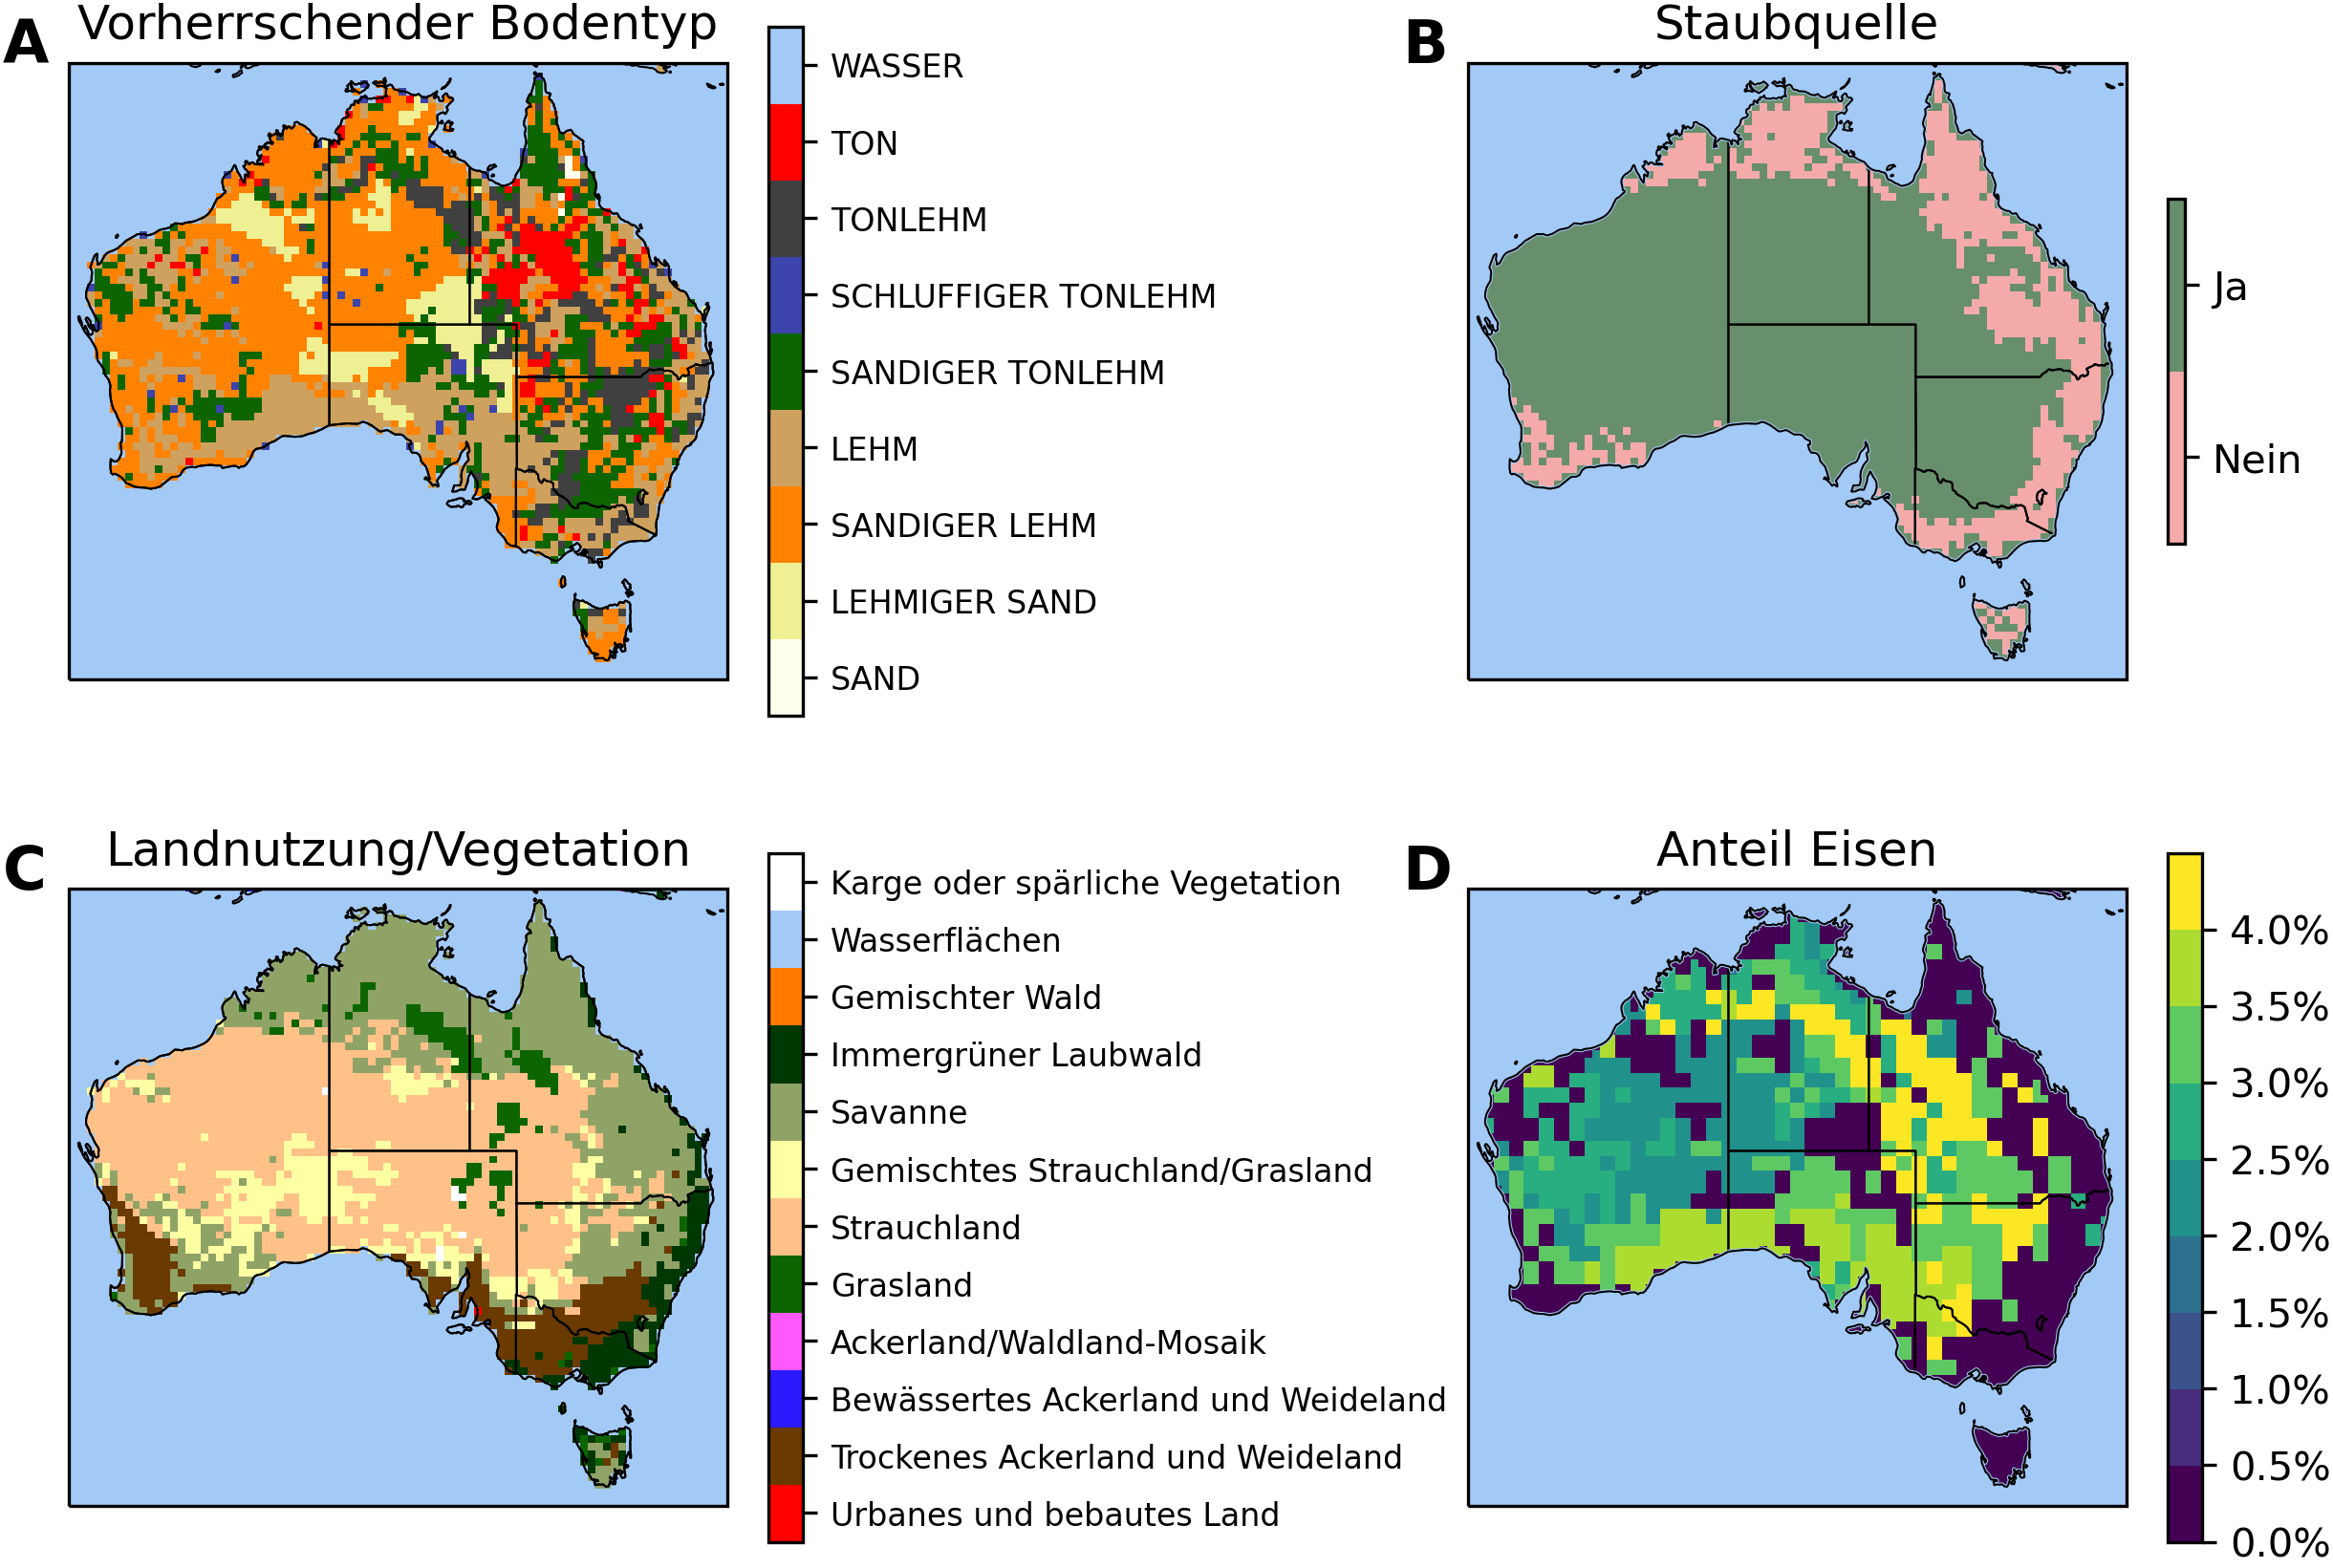
\includegraphics[width=\textwidth]{bilder/soil_type_iron.png}
\caption{Zusammenstellung einiger Parameter, wie sie dem WRF-Modell auf Basis von GIS-Daten übergeben wurden. A) Vorherrschender Bodentyp gemäß STAS-Klassifizierung. B) Staubquellen, die Gitterpunkte nehmen entweder den Wert 0 oder 1 an. C) Landnutzung/Vegetationstyp gemäß USGS-Klassifizierung (United States Geological Survey). D) Eisenanteil im Sediment, beispielhaft für Korngrößenklasse 1 (sh. Tabelle \ref{table:wrf}). Die anderen Korngrößen weisen geringere Werte, aber räumlich dieselbe Verteilung auf.} \label{fig:soil_type_iron}
\end{figure}
Für die Untersuchung im Rahmen dieser Arbeit ist wieder entscheidend, dass diese Eisenressourcen im Sediment häufig in der für Phytoplankton kaum verfügbaren oxidierten Form Fe$^{3+}$ als Mineral Hämatit Fe$_2$O$_3$ und Goethit $\alpha$-Fe$^{3+}$O(OH) vorkommen \citep{Reynolds.2014}. Transportprozesse und Wolkenbildungen können die Transformation zu einer löslicheren Form jedoch fördern \citep{Shao.2011}. Hauptursache für die Ablagerung von sehr weit transportiertem Staub ist laut \citet{Marx.2018} das \textit{Auswaschen} durch Regen. Wird Staub über mehrere tausend Kilometer transportiert, verbleiben außerdem  i.d.R. nur Staubpartikel mit Größen von $<$20$\mu$m \citep{Marx.2018}). Im Gegensatz zu den meisten anderen Plankton-Arten wurde beobachtet, dass \textit{Trichodesmium} die Rate des Eisenauflösens von Oxiden und Staub beschleunigen kann \citep{Rubin.2011}.
\subsubsection{Beschreibung des Staubsturms im September 2009} \label{sec:reddawn}
Bereits nach einer schnellen Analyse im Rahmen des DustWatch Reports \citep{Leys.2009} war klar, dass es sich bei \textit{Red Dawn} um einen außerordentlichen Staubsturm mit besonderen Merkmalen handelte. Den Namen \textit{Red Dawn} erhielt dieser aufgrund der spektakulären Bilder die er am Morgen (Lokalzeit, vgl. mit Satellitenbild \ref{fig:satellite} B)) des 23. Septembers in Sydney verursachte. Die komplette Stadt wurde für mehrere Stunden in orange-roten Nebel gehüllt (Abb. \ref{fig:reddawn}). Tatsächlich fanden im September sowohl vor als auch nach dem hier im Fokus liegenden \textit{Red Dawn} gleich mehrere Staubereignisse statt (sh. Auswertung, Kapitel \ref{sec:auswertung}). Im ariden Inland sind Staubstürme keine Seltenheit. Dieses war allerdings (jedenfalls in Bezug auf die Sichtweiten-Reduzierung) das stärkste Staubereignis welches die Küstenstadt Sydney seit Beginn verlässlicher Aufzeichnungen (1940) getroffen hat \citep{Leys.2011}. Vorangegangen sind Monate und Jahre mit im Vergleich zum Durchschnitt höheren Temperaturen und unterdurchschnittlichem Niederschlag (vgl. Abbildung \ref{fig:reddawn}), wodurch die Vegetation schwächer ausgeprägt und die Erdböden allgemein trockener waren \citep{Leys.2011}. Aufgrund der hohen Intensität wurde dieser Zeitraum \textit{Millenium Drought} getauft \citep{Deckker.2014}.
\begin{figure}[htbp]
	\begin{minipage}[c]{0.5\textwidth}
		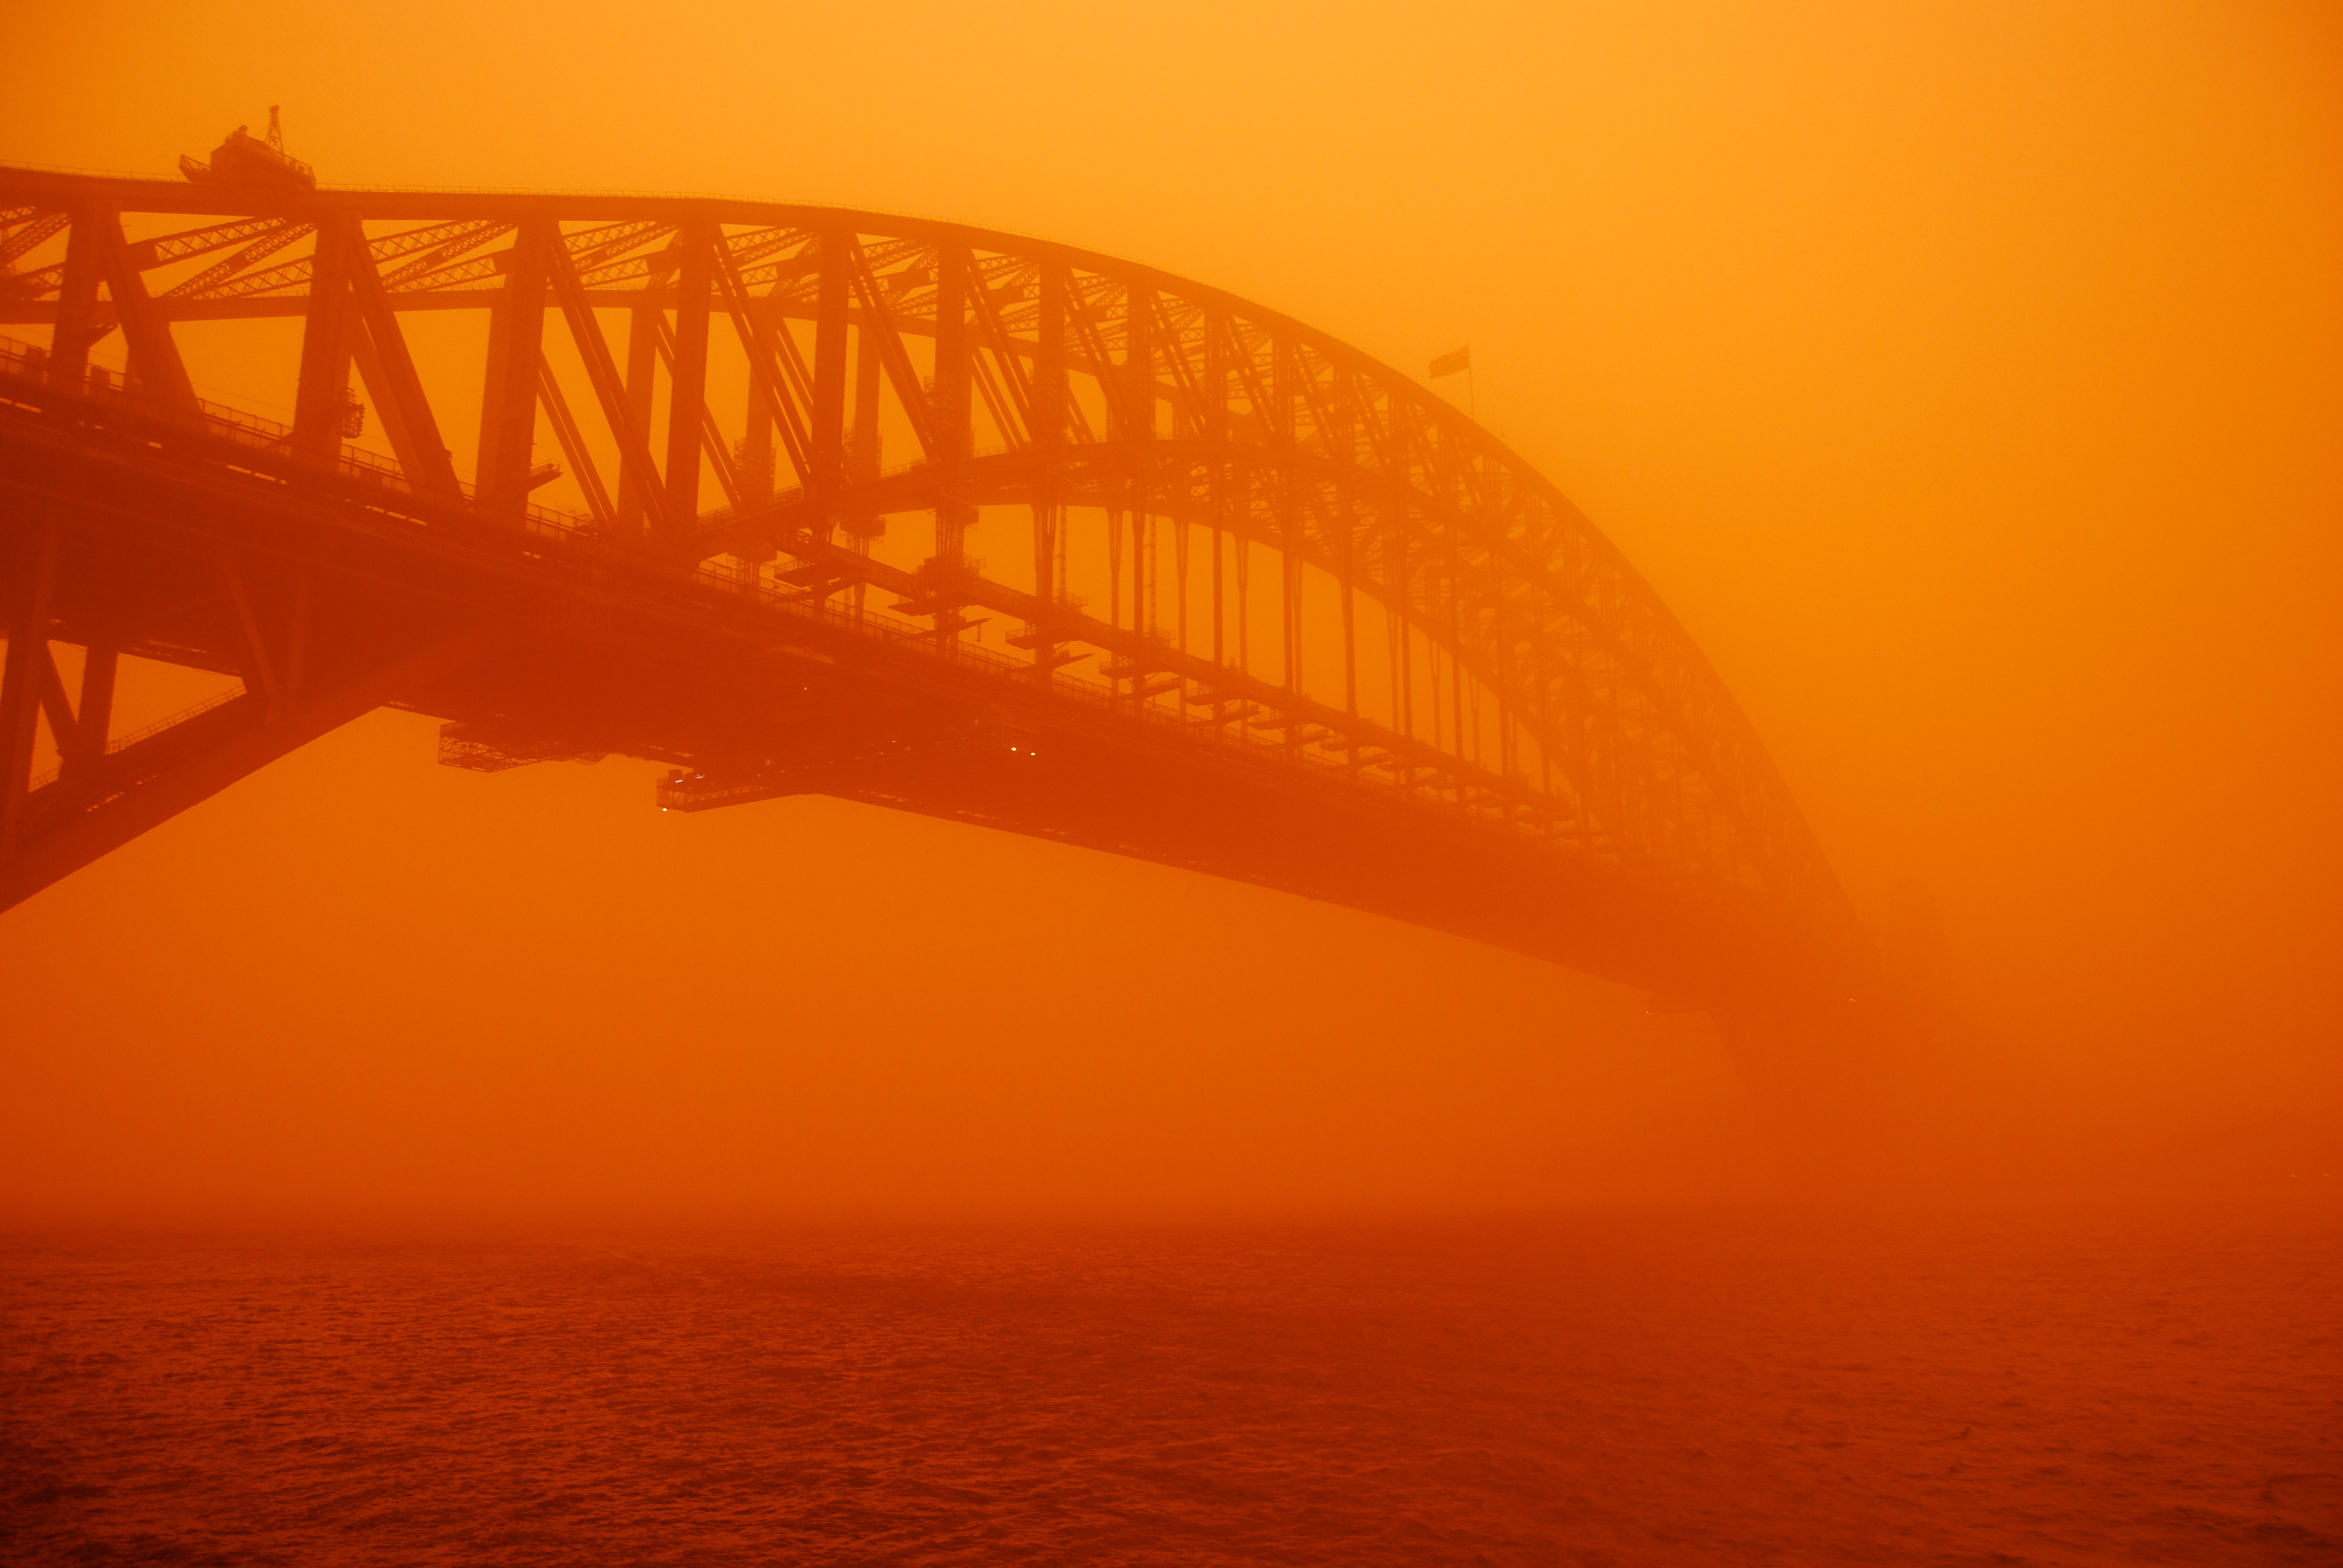
\includegraphics[width=\textwidth]{bilder/reddawn/SHB.jpg}
	\end{minipage}\hfill
	\begin{minipage}[c]{0.49\textwidth}
		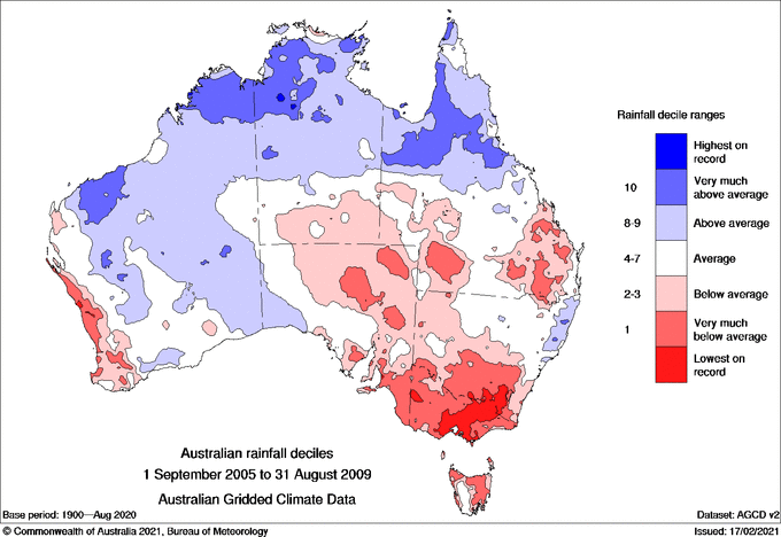
\includegraphics[width=\textwidth]{bilder/reddawn/drought.png}
	\end{minipage}\hfill
	\caption{Links: Aufnahme der Sydney Harbour Bridge während des Red Dawn Events (https://en.wikipedia.org/wiki/2009_Australian_dust_storm). Rechts: Regenfälle in Dezilen für die letzten 4 Jahre vor Red Dawn. Dunkelrot: 90 \% der Vergleichszeiträume hatten mehr Regen in dieser Region, dunkelblau: 90 \% der Vergleichszeiträume hatten weniger Regen.} \label{fig:reddawn}
\end{figure}
Dieses Klima bot entsprechend günstige Bedingungen für die Entstehung eines Staubsturms. Auf Abbildung \ref{fig:bom_analysis} ist das Tiefdruckgebiet dargestellt, welches mit den starken Emissionen in Verbindung gebracht wird. Einen Tag vor dem eigentlichen Ereignis befindet es sich direkt südlich von Südaustralien, bereits losgelöst von der südlichen Polarfront. Zu diesem Zeitpunkt wird bereits Staub über die Ostküste in Richtung Tasmanisches Meer transportiert (sh. Abb. \ref{fig:satellite} A). Aus diesem Tiefdruckgebiet und der zugehörigen Kaltfront (blau) resultiert Wind in Sturmstärke (sh. Abb. \ref{fig:wind_reddawn}), welcher die Höhe der planetaren Grenzschicht verändert \citep{AlizadehChoobari.2012} und so den Staub in die Atmosphäre abträgt. Anschließend wird dieser hauptsächlich in Richtung Ostküste weitertransportiert (\cite{Leys.2011}, Abb. \ref{fig:satellite} C+D). \citet{Leys.2011} schätzen, dass 2.54 Tg Staub über die Küste hinaus transportiert wurden. Es wurden verschiedene Quellen identifiziert, welche im Rahmen des Ereignisses Staub emittiert haben sollen:
\begin{itemize}
\item Unteres Lake Eyre Becken in Südaustralien (\cite{Leys.2011}, \cite{Leys.2009}) (Staub aus Canberra: Lake Torrins gem. \cite{Deckker.2014})
\item Bergbaugebiete um Cobar und Broken Hill  (\cite{Leys.2011})
\item Weideland im Nordwesten von New South Wales (\cite{Leys.2011}, \cite{Leys.2009})
\item Channel Country in Queensland (\cite{Leys.2011},\cite{Leys.2009})
\end{itemize}
\citet{Leys.2011} folgern, dass neben den trockenen Seen- und Flusslandschaften als gewöhnliche Quellen, insbesondere Weideland und Sandflächen Staub emittiert und letztlich zu der bemerkenswerten rötlichen Färbung geführt haben könnten.
\begin{figure}[htbp]
	\begin{minipage}[c]{0.33\textwidth}
		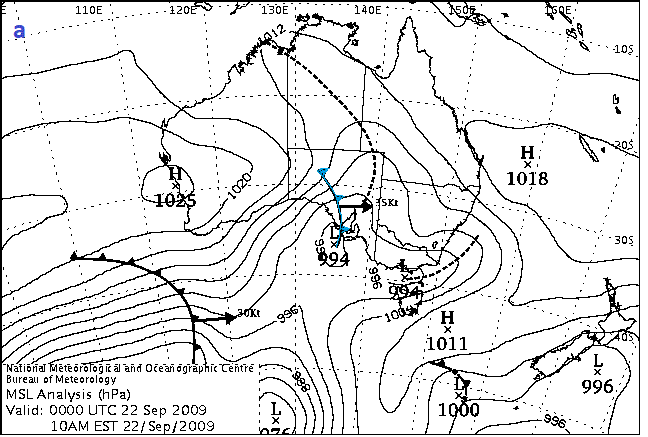
\includegraphics[width=\textwidth]{bilder/reddawn/2009092200.png}
	\end{minipage}\hfill
	\begin{minipage}[c]{0.33\textwidth}
		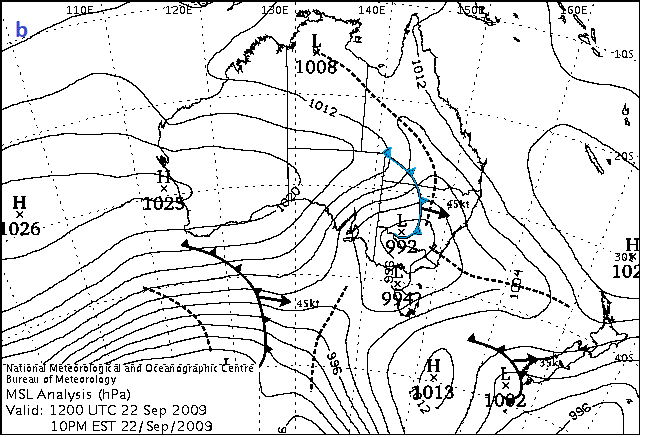
\includegraphics[width=\textwidth]{bilder/reddawn/2009092212.png}
	\end{minipage}\hfill
		\begin{minipage}[c]{0.33\textwidth}
		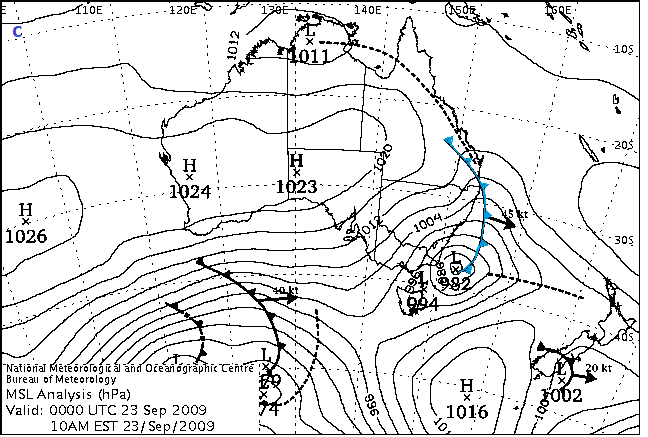
\includegraphics[width=\textwidth]{bilder/reddawn/2009092300.png}
	\end{minipage}\hfill
	\caption{Bodendruck- und Fronten-Analysen des australischen \textit{Bureau of Meteorology} für a) den 22.09.2009 um 0 Uhr UTC, b) später um 12 Uhr UTC und c) der 23.09.2009 wieder um 0 Uhr UTC. Die Kaltfront, die mutmaßlich für die starken Staubemissionen bzw. den sogenannten \textit{Red Dawn} in Sydney geführt hat, wurde nachträglich blau gekennzeichnet.} \label{fig:bom_analysis}
\end{figure}
\begin{figure}[htbp]
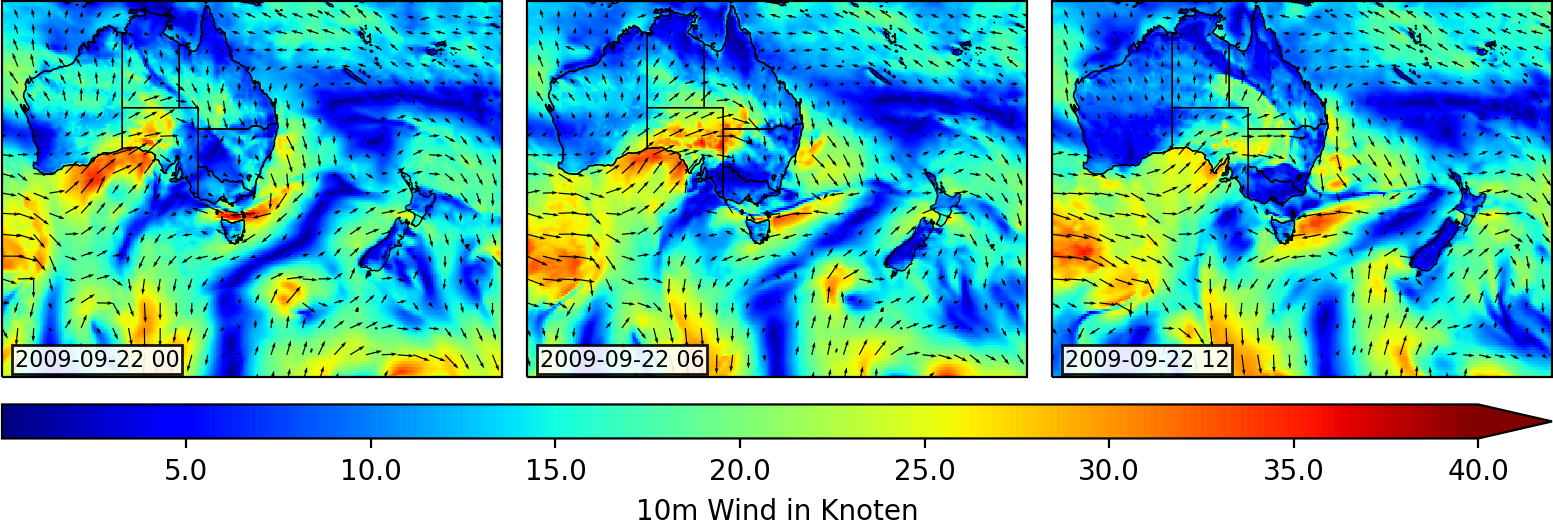
\includegraphics[width=\textwidth]{bilder/reddawn/wind_reddawn_small.png}
\caption{Windgeschwindigkeiten zu den Zeitpunkten der Staubemissionen vom 22.09. 0 Uhr UTC bis 12 Uhr UTC. Im südlichen Lake Eyre Becken erreicht der Wind gegen 6 Uhr UTC Sturmstärke.} \label{fig:wind_reddawn}
\end{figure}
\begin{figure}[htbp]
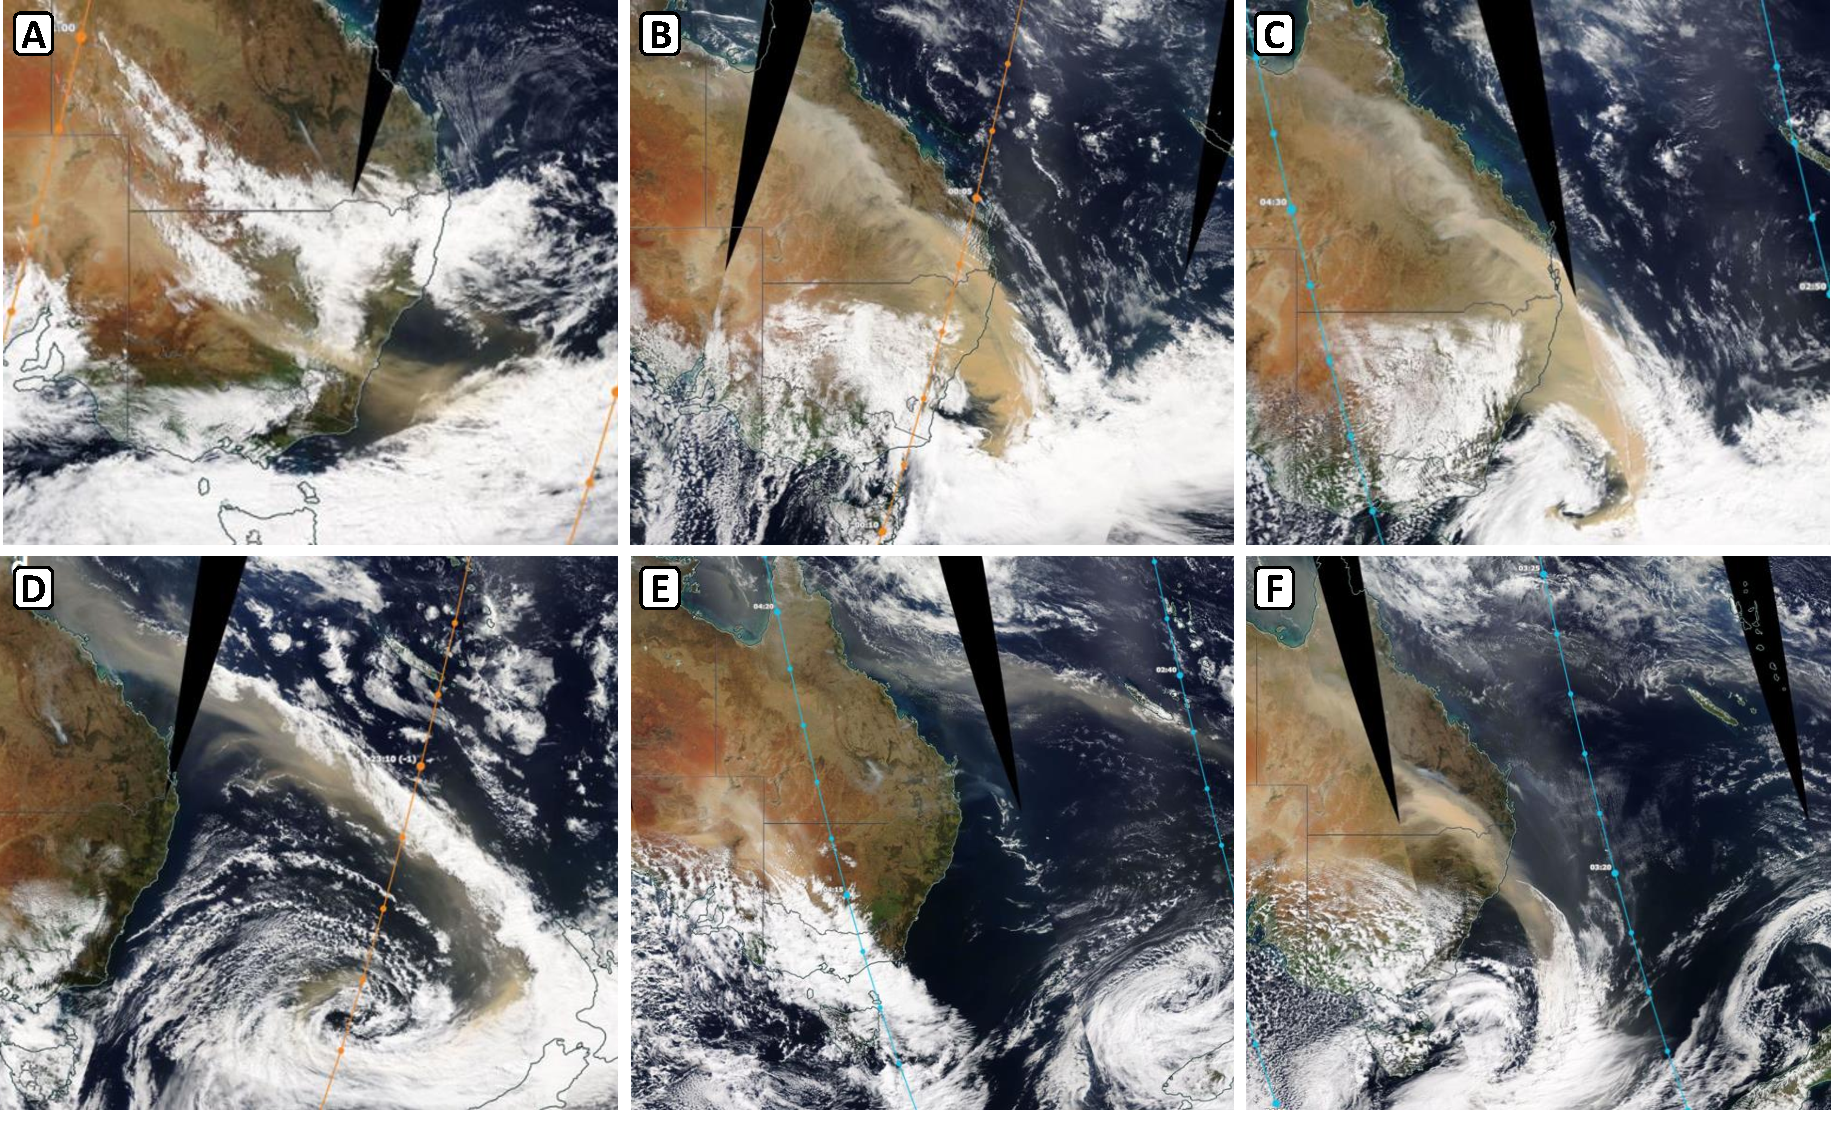
\includegraphics[width=\textwidth]{bilder/reddawn/reddawn_satellite.pdf}
\caption{Aufnahmen der Satelliten AQUA und TERRA des östlichen Teils des australischen Kontinents während der Staubereignisse. A) Noch vor dem eigentlichen Red Dawn Event am 22.09. um ca. 1 Uhr UTC, B) Staubwolke mit maximaler Intensität zum Red Dawn am 23.09. um etwa 0 Uhr UTC, C) ca. 4 Stunden später mit ähnlicher Ausdehnung, D) Staubwolke deutlich im Einfluss des Tiefdruckgebiets am 24.09. um 0 Uhr UTC, E) Staub verteilt in der Atmosphäre am 25.09. um ca. 4 Uhr UTC und F) das nächste Ereignis verbunden mit neuen Emissionen am 26.09. um ca. 3 Uhr UTC.} \label{fig:satellite}
\end{figure}
Mit dem Ereignis geht mäßiger bis starker Niederschlag (max. knapp 10mm/h am Morgen des 23.09.) in insgesamt moderater Summe einher (sh. Abb. \ref{fig:rain}). Dieser fällt im Süden von New South Wales, ist aber erst im Tasmanischen Meer maximal. Ein Teil der Staubwolke befindet sich innerhalb dieser Zone des Niederschlags (vgl. Abb. \ref{fig:satellite} B bis D). Regen führt zu nassem Eintrag bzw. \textit{Auswaschen} des Staubs, was  für die Löslichkeit des eingebrachten Staubs eine entscheidende Rolle spielen kann \citep{Shao.2011}. \citet{Reynolds.2014} folgern, dass der Eisengehalt (Magnetit Fe$_2$O$_4$) des Staubes beim \textit{Red-Dawn} durch die dichten urbanen Gebiete an der Küste weiter erhöht wurde. Einen Tag später ist der mit dem \textit{Red Dawn} verbundene Staub auf den Satellitenbildern deutlich weniger präsent (Abb. \ref{fig:satellite} E), bis am 26.09. erneut Staub vom Festland über den Ozean getragen wird (Abb. \ref{fig:satellite} F).
\begin{figure}[htbp]
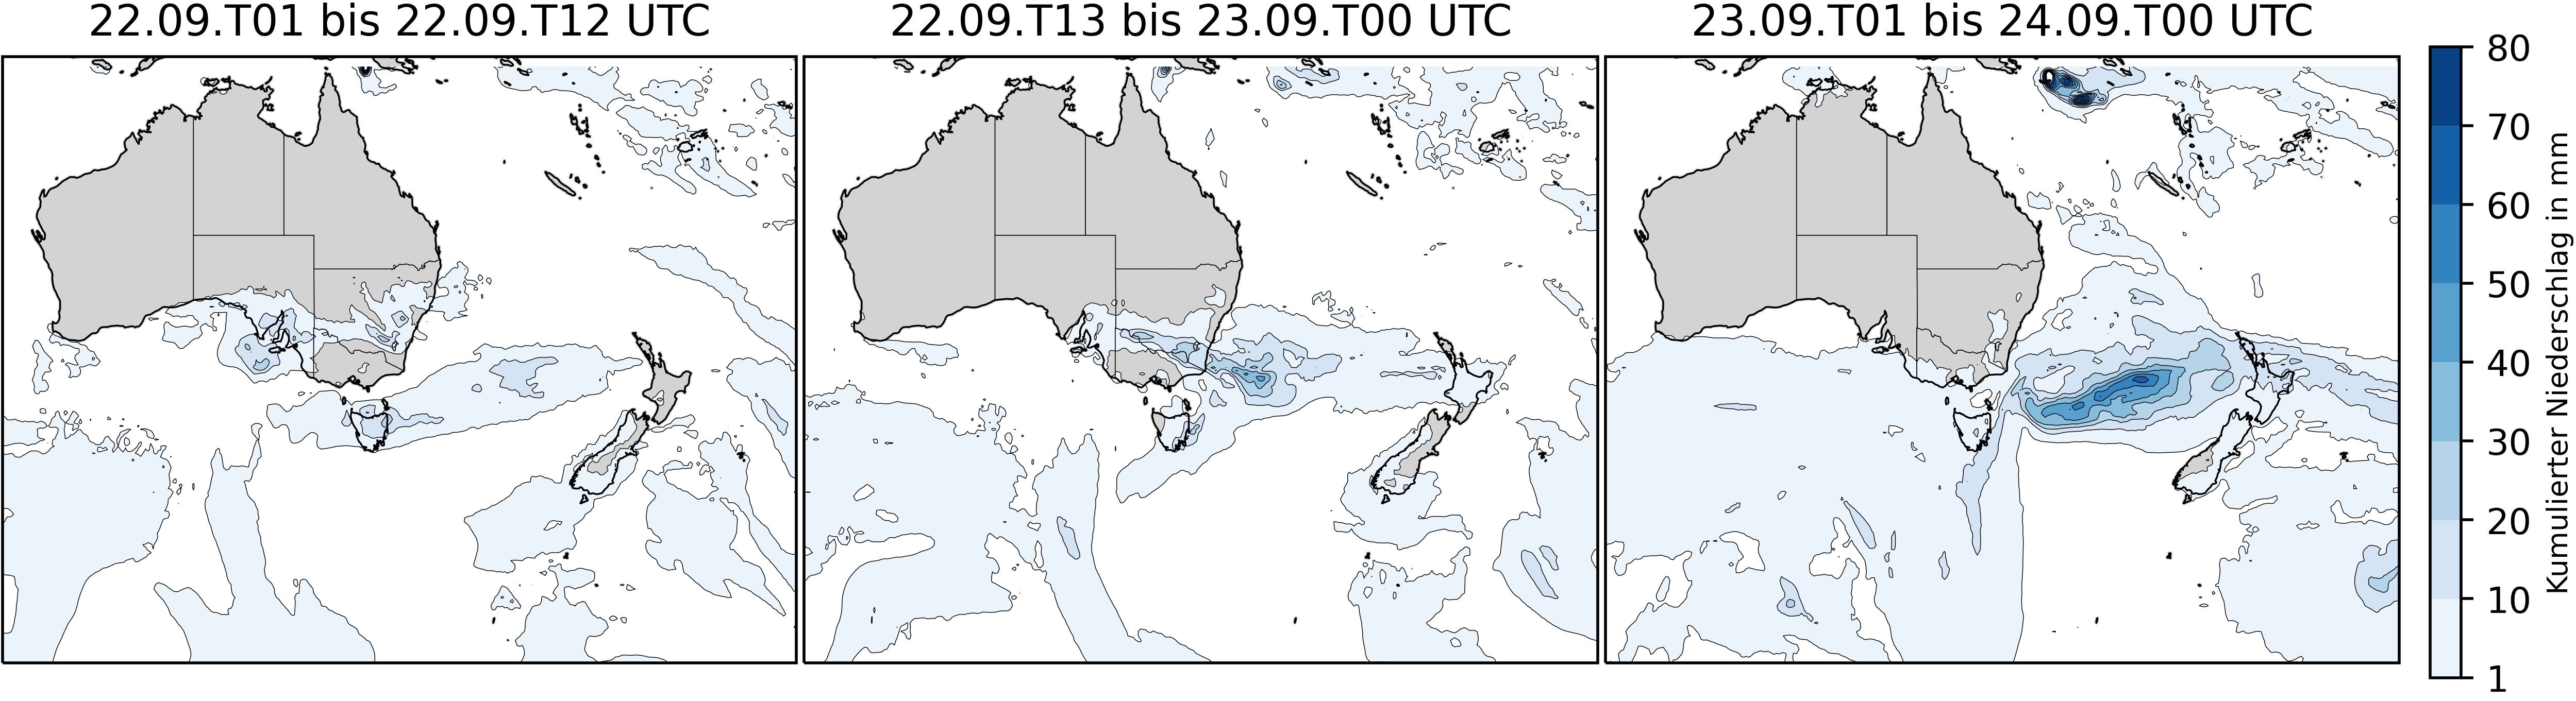
\includegraphics[width=\textwidth]{bilder/reddawn/rain.png}
\caption{Kumulierter Niederschlag im Zusammenhang mit \textit{Red Dawn} bzw. dem assoziierten Tiefdruckgebiet mit der Kaltfront aus Reanalyse-Daten, sh. Tabelle \ref{table:data}.} \label{fig:rain}
\end{figure}
\subsection{Bisherige Arbeiten zum Zusammenhang zwischen Staubereignissen und Phytoplankton}
Aufgrund der bekannten Eigenschaft, dass Eisen grundsätzlich düngend wirken kann und der möglicherweise erheblichen Bedeutung für die globale Klimageschichte (Kapitel \ref{sec:Eisenhypothese}), beschäftigten sich bereits mehrere Arbeiten mit der Untersuchung eines Zusammenhangs zwischen Staub-Niederschlägen und Phytoplankton-Wachstum. \citet{Boyd.2010} schätzen allerdings in einer kurzen Revision ein, dass einige der Ergebnisse wenig belastbar sind oder gar falsch interpretiert wurden. Dadurch, dass die eisenhaltigen Minerale im Ozeanwasser kaum bzw. nur sehr langsam gelöst werden, seien echte staub-gesteuerte Phytoplankton-Blüten selten. Die schwache Löslichkeit kann sich lt. \citet{Boyd.2010} jedoch in Langzeitfolgen auswirken, sodass bspw. reguläre saisonale Phytoplankton-Blüten früher eintreten und andauern oder die Eisenkonzentrationen durch die langsame, stetige Auflösung der Minerale ansteigen, bis eine Schwelle erreicht wird, bei welcher diese dann konsumiert werden. Die dabei angenommene Verweilzeit der Eisenpartikel im Oberflächenwasser ist entsprechend lang (Tage bis Monate). In bisherigen Arbeiten wurden einige Zusammenhänge aufgezeigt, wovon mehrere auch für diese Arbeit von Relevanz sind, sodass hier ein kurzer Auszug vorgestellt wird. Im Kontrast zu den vorgenannten Langzeitprozessen identifizieren \citet{Shaw.2008} bereits direkt mit (bzw. sogar kurz vor) Eintreffen des weiteren prominenten australischen Staubsturmes im Oktober 2002 Reaktionen der Chlorophyll-a-Konzentrationen vor der Küste Queenslands. Häufiger scheinen die Reaktionen jedoch ähnlich zu den \textit{Bottle Experiments} von \citet{Martin.1988} und den Düngungs-Experimenten \citep{Trull.2001} nach einigen wenigen Tagen beobachtbar zu sein: \citet{Bali.2019} zeigen in einer Korrelationsanalyse für einen Staubsturm im Arabischen Meer 2012 einen Chlorophyll-Peak nach 4 Tagen und folgern einen zusätzlichen Effekt durch eine Vertiefung der MLD aufgrund der Abkühlung des Oberflächenwassers durch die Staubpartikel. Auch \citet{Bishop.2002} beschreiben einen Anstieg der Biomasse etwa 5 Tage nach einem der Wüste Gobi entsprungenen Staubsturm mit Eintrag in den subarktischen Pazifik 2001. In diesem Fall bleib die Biomasse über beinahe zwei Wochen annähernd verdoppelt und nahm etwa zwei Wochen nach dem Eintrag die maximalen Konzentrationen an. Nach einem Staubsturm im März 2010, der mutmaßlich große Mengen Staub in das Gelbe Meer bei China eingetragen hat, beschreiben \citet{Tan.2014} die Reaktionen jedoch erst später, etwa 10-13 Tage nach dem Ereignis, mit einem Maximum nach erst 36 Tagen. \citet{Shi.2012} untersuchen ebenfalls die Auswirkungen eines Staubsturms im Frühling 2007 mit Auswirkungen auf das Gelbe Meer, identifizieren eine Phytoplankton-Blüte allerdings bereits 3-4 Tage nach dem Ereignis. Von besonderer Relevanz ist außerdem noch die Veröffentlichung von \citet{Gabric.2016}, welche dasselbe Staubereignis analysiert, wie  diese Arbeit. Die Analyse beschränkt sich allerdings auf das Tasmanische Meer und es werden keine expliziten Aussagen zu einer Reaktionszeit des Phytoplanktons getroffen. Dennoch werden gesteigerte Chlorophyll-a-Konzentrationen beobachtet und auf das \textit{Red Dawn Event} zurückgeführt. \citet{Gabric.2016} berücksichtigen dabei qualitativ die lokalen Besonderheiten des Tasmanischen Meeres und schreiben dem Staubeintrag aufgrund von Niederschlägen eine besondere Rolle zu. Insgesamt lässt sich festhalten, dass etwaige Reaktionen des Phytoplanktons nicht überall gleichermaßen beobachtbar sind, nach unterschiedlichen Zeiträumen eintreten können und offenbar von  weiteren Faktoren abhängig sind. 
\section{Methoden und Daten} \label{sec:Methoden}
Um testen zu können, ob ein extremes Staubereignis Auswirkungen auf die Phytoplanktonproduktion in einer bestimmten Region hat, ist eine geeignete Datenbasis erforderlich. Grundsätzlich müssen hierzu zwei Variablen räumlich und zeitlich aufgelöst werden: Staubeintrag und Phytoplankton-Konzentrationen. In beiden Fällen ist die Auflösung in jeder dieser Dimensionen stark beschränkt. Speziell Ausdehnung und Trajektorien von Staubstürmen müssen aufgrund der spärlichen Beobachtungsdaten (siehe Kapitel  \ref{sec:reddawn}) größtenteils geschätzt werden. Simulationen leistungsfähiger Modelle können die Abschätzungen jedoch verbessern. Im Rahmen dieser Arbeit wird eine spezielle WRF-Simulation (sh. Kapitel \ref{sec:wrf}) verwendet, um genauere Aussagen über das Verhalten der Staubwolke und den späteren Eiseneintrag treffen zu können. Die Konzentrationen des Phytoplanktons werden aus satellitengestützten täglichen Messungen der Chlorophyll-a-Konzentrationen abgeleitet (sh. Kapitel \ref{sec:chla}). Für den finalen Test eines möglichen Zusammenhangs werden die in Kapitel \ref{sec:stats} vorgestellten statistischen Methoden angewendet.
\subsection{WRF-Modell} \label{sec:wrf}
Das \textit{Weather Research and Forecasting} (WRF) Modell ist ein mesoskaliges System zur numerischen Wettersimulation. Es findet in der Atmosphärenforschung breite Anwendung und kann für verschiedene Zwecke mit einer Auflösung von weniger als einem Meter bis hin zu mehreren tausend Kilometern eingesetzt werden \citep{NCAR.2021}. Im Rahmen dieser Arbeit wurden die Ergebnisse einer WRF-Simulation verwendet, welche um ein Modul ergänzt wurde, das neben den üblichen meteorologischen Größen auch Staub-Emission, -Transport und -Niederschlag berücksichtigt. Dieses WRF-Modell der Version 4.1.2 simuliert darüber hinaus auf Basis der Bodentypen (vgl. Abb. \ref{fig:soil_type_iron}) die im Staub enthaltenen Eisenkonzentrationen. Als Staub-Emissionsschema wurde jenes von \citet{Shao.2004} verwendet. Das Modell berechnet die Staubkonzentrationen für 5 verschiedene Korngrößenklassen, welche in Tabelle \ref{table:wrf} dargestellt sind. Simuliert wurde der Zeitraum vom 18.09.2009 um 0 Uhr UTC bis zum 30.09.2009 um 0 Uhr UTC. Die verfügbaren Variablen werden in der Ausgabedatei in einem Intervall $\Delta t$ von drei Stunden gespeichert, wodurch sich insgesamt $N_t = 97$ auswertbare Zeitschritte ergeben. Zum Startzeitpunkt werden dem Modell keine Anfangs-Staubkonzentrationen übergeben, es wird also angenommen, dass zu diesem Zeitpunkt kein Staub in der Atmosphäre ist. Emissionen zu früheren Zeitpunkten werden dadurch vernachlässigt. Räumlich deckt das Modell von 110.3° Ost bis 170.3° West und von 57.06° S bis 9.89° S den gesamten australischen Kontinent, das Tasmanische Meer, Neuseeland und Teile des südlichen Ozeans und Pazifiks ab. Dieses Gebiet wird mit 164$\times$124 (Ost-West$\times$Süd-Nord) Gitterpunkten abgedeckt. Ein Gitterpunkt repräsentiert damit ein Gebiet von etwa 53.3 km$\times$53.1 km (am nördlichsten Punkt in der Domäne, im Süden sind es 29.4 km$\times$29.5 km). Mehrere Größen, die für Emission, Transport und Niederschlag wichtig sind (bspw. lokale Form des Geländes, steile Topographie, Rauheit, Turbulenzen), können nicht aufgelöst werden und müssen im Modell parametrisiert werden. Die vertikale Verteilung wird auf 32 Höhenlevel simuliert. Das unterste Höhenlevel ist (entsprechend der Auflösung) geländefolgend, das oberste liegt oberhalb der Troposphäre zwischen 19.044 m und 20.230 m über Meeresniveau.
\begin{table}[H]
\caption{Die Staubpartikel wurden in verschiedene Korngrößen unterteilt. Alle relevanten Variablen wurden jeweils für jede Größenklasse separat ausgegeben.} \label{table:wrf}
\centering
\begin{tabularx}{\textwidth}{l l X}
		\toprule
			\thead{Größen-\\klasse} & \thead{Effektiver\\ Radius} & \thead{Verfügbare Variablen für alle Größen (Auszug)} \\
		\midrule
		1 & $0.5 \ \mu$m & atmosphärische Staub-/Eisenkonzentrationen,  \\
		2 & $1.4 \ \mu$m & nasser, trockener und gravitativer Eintrag,\\
		3 & $2.4 \ \mu$m & Eisengehalt Bodentypen, Emissionen \\
		4 & $4.5 \ \mu$m &..\\
		5 & $8.0 \ \mu$m  \\
		\bottomrule
\end{tabularx}
\end{table}
\subsection{Chlorophyll a} \label{sec:chla}
Um die Taxonomie und die genauen Konzentrationen des Phytoplanktons im Meerwasser abzuleiten, sind in situ Messungen erforderlich. Für die Untersuchung eines Zusammenhangs in dieser Arbeit ist es allerdings ausreichend, die grundsätzliche Tendenz der Entwicklung der Phytoplankton-Konzentrationen zu quantifizieren. Eine explizite Kenntnis der speziellen Zusammensetzung ist nicht erforderlich, kann aber anhand vorangegangener Untersuchungen und der für die jeweilige Region erwartbaren Verteilungen abgeschätzt werden. Messungen des in Pflanzen enthaltenen Farbstoffs Chlorophyll erlauben, Produktion und Konzentrationen des Phytoplanktons abzuleiten \citep{RYTHER.1957}. Dementsprechend ist es zu diesem Zweck üblich, die Nettoprimärproduktion aus Satellitenmessungen abzuleiten, welche Werte des Hauptpigments \textit{Chlorophyll-a} ausgeben. Da die Reaktionszeit auf möglichen \textit{Dünger} mit 4-5 Tagen und die Lebensdauer (vgl. Kapitel \ref{sec:Phytobasics}) relativ kurz sind, ist es vorteilhaft, zeitlich möglichst hoch aufgelöste, tägliche Daten zu verwenden. Eine erhebliche Einschränkung dieser satellitengestützten Daten ist, dass die Beobachtungen nur über eis- und wolkenfreiem Himmel möglich sind. Zusätzlich kann reflektiertes Sonnenlicht die Ableitung erschweren. Auf Abbildung \ref{fig:chla} wird beispielhaft demonstriert, dass diese Faktoren zu einer sehr schlechten räumlichen Auflösung führen können. Glücklicherweise bieten der \textit{Copernicus Marine Service} bzw. \citet{Saulquin.2019} einen überarbeiteten Datensatz für den Betrachtungszeitraum, welcher die fehlenden Beobachtungsdaten mithilfe aktueller Algorithmen in täglicher Auflösung interpoliert. Obwohl dieser Datensatz die gewässertypischen Besonderheiten berücksichtigt und auf Basis fundierter Interpolationsmethoden zusammengestellt wurde, muss aufgrund der begrenzten Abdeckung (insbesondere südlich des australischen Kontinents) bei der späteren Interpretation ein entsprechend hoher möglicher Fehler bedacht werden. Die Werte werden aus den Messungen mehrerer Sensoren/Spektrometer (MERIS, MODIS und SeaWiFS) zusammengestellt. Unter zusätzlicher Berücksichtigung der Temperatur des Oberflächenwassers, der einfallenden Sonnenstrahlung, der Tiefe der \textit{Mixed Layer}, Up- und Downwellingzonen (wie (anti-)zyklonalen Wirbeln) können anschließend aus den Chlorphyll-a-Konzentrationen die Nettoprimärproduktion, also Phytoplanktonwachstum abgeleitet werden \citep{Falkowski.1998}. Letztere Umrechnung erfolgt im Rahmen dieser Arbeit nicht. Veränderungen der Chlorophyll-a-Konzentrationen werden mit Veränderungen des Phytoplankton-Bestands gleichgesetzt.
\begin{figure}[htbp]
	\begin{minipage}[c]{0.49\textwidth}
		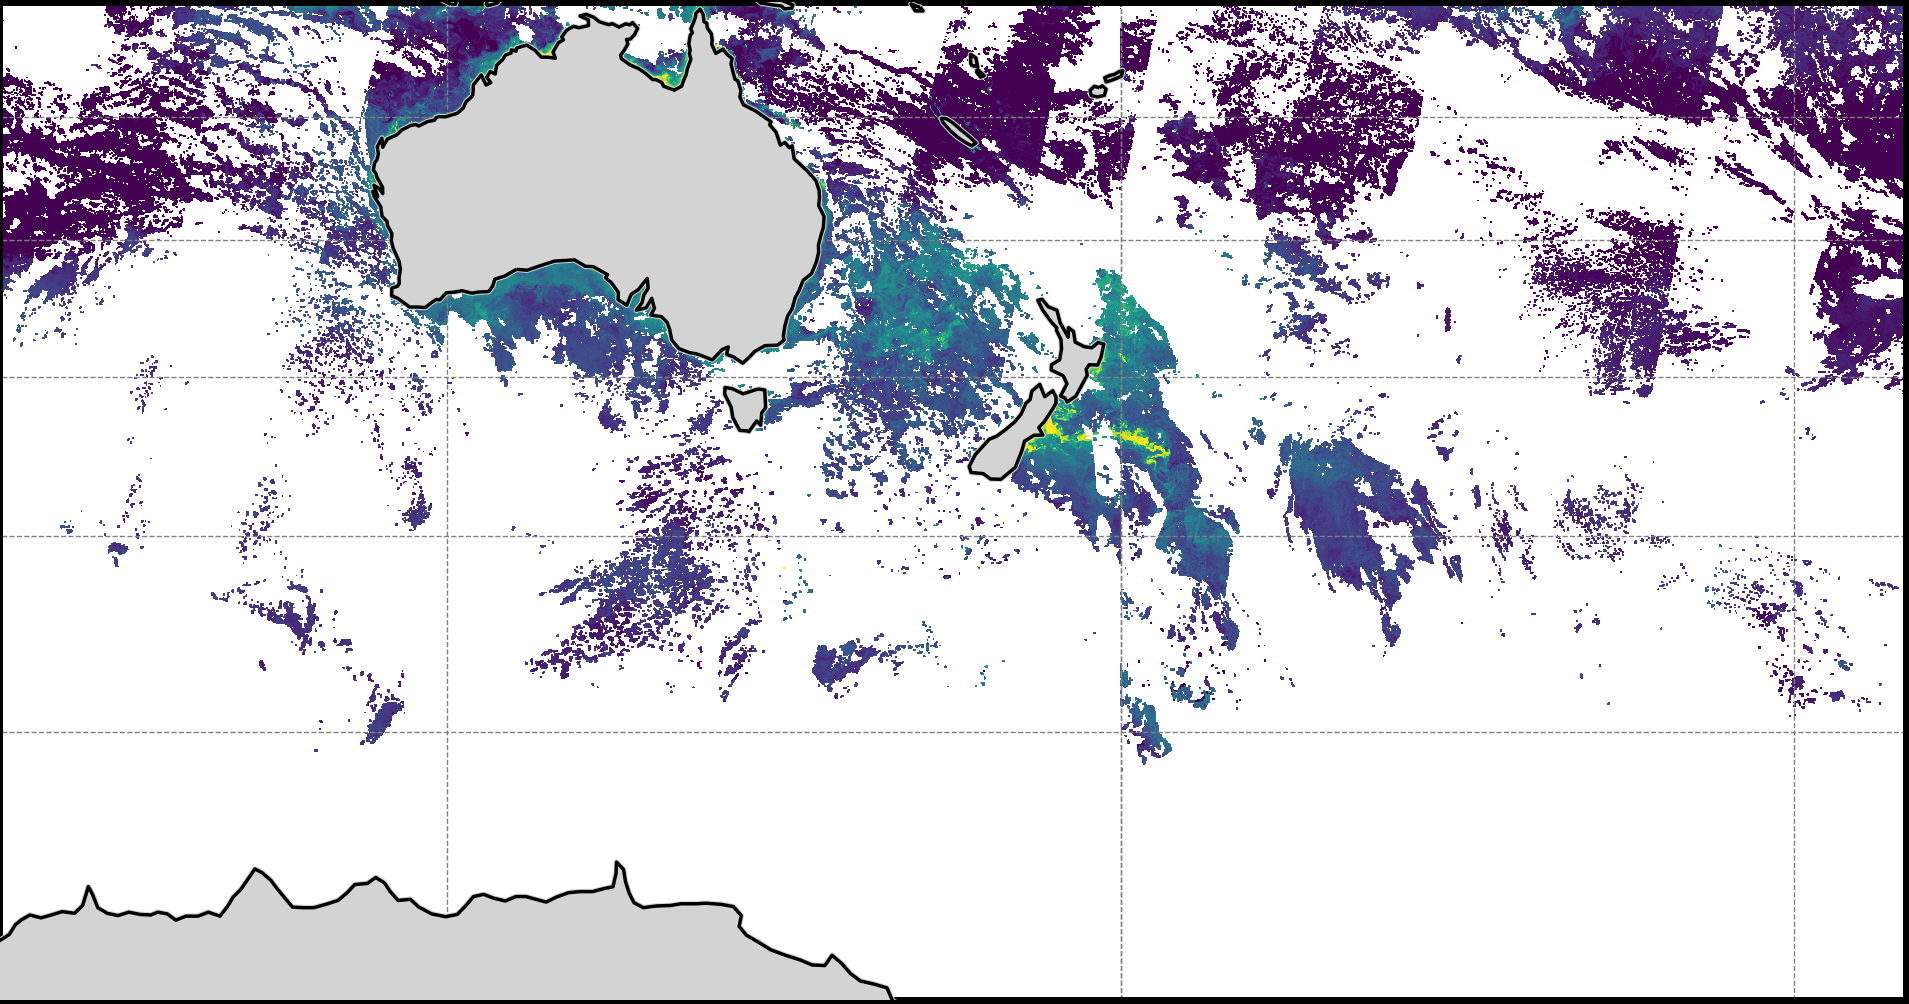
\includegraphics[width=\textwidth]{bilder/chla_raw.png}
	\end{minipage}\hfill
	\begin{minipage}[c]{0.49\textwidth}
		 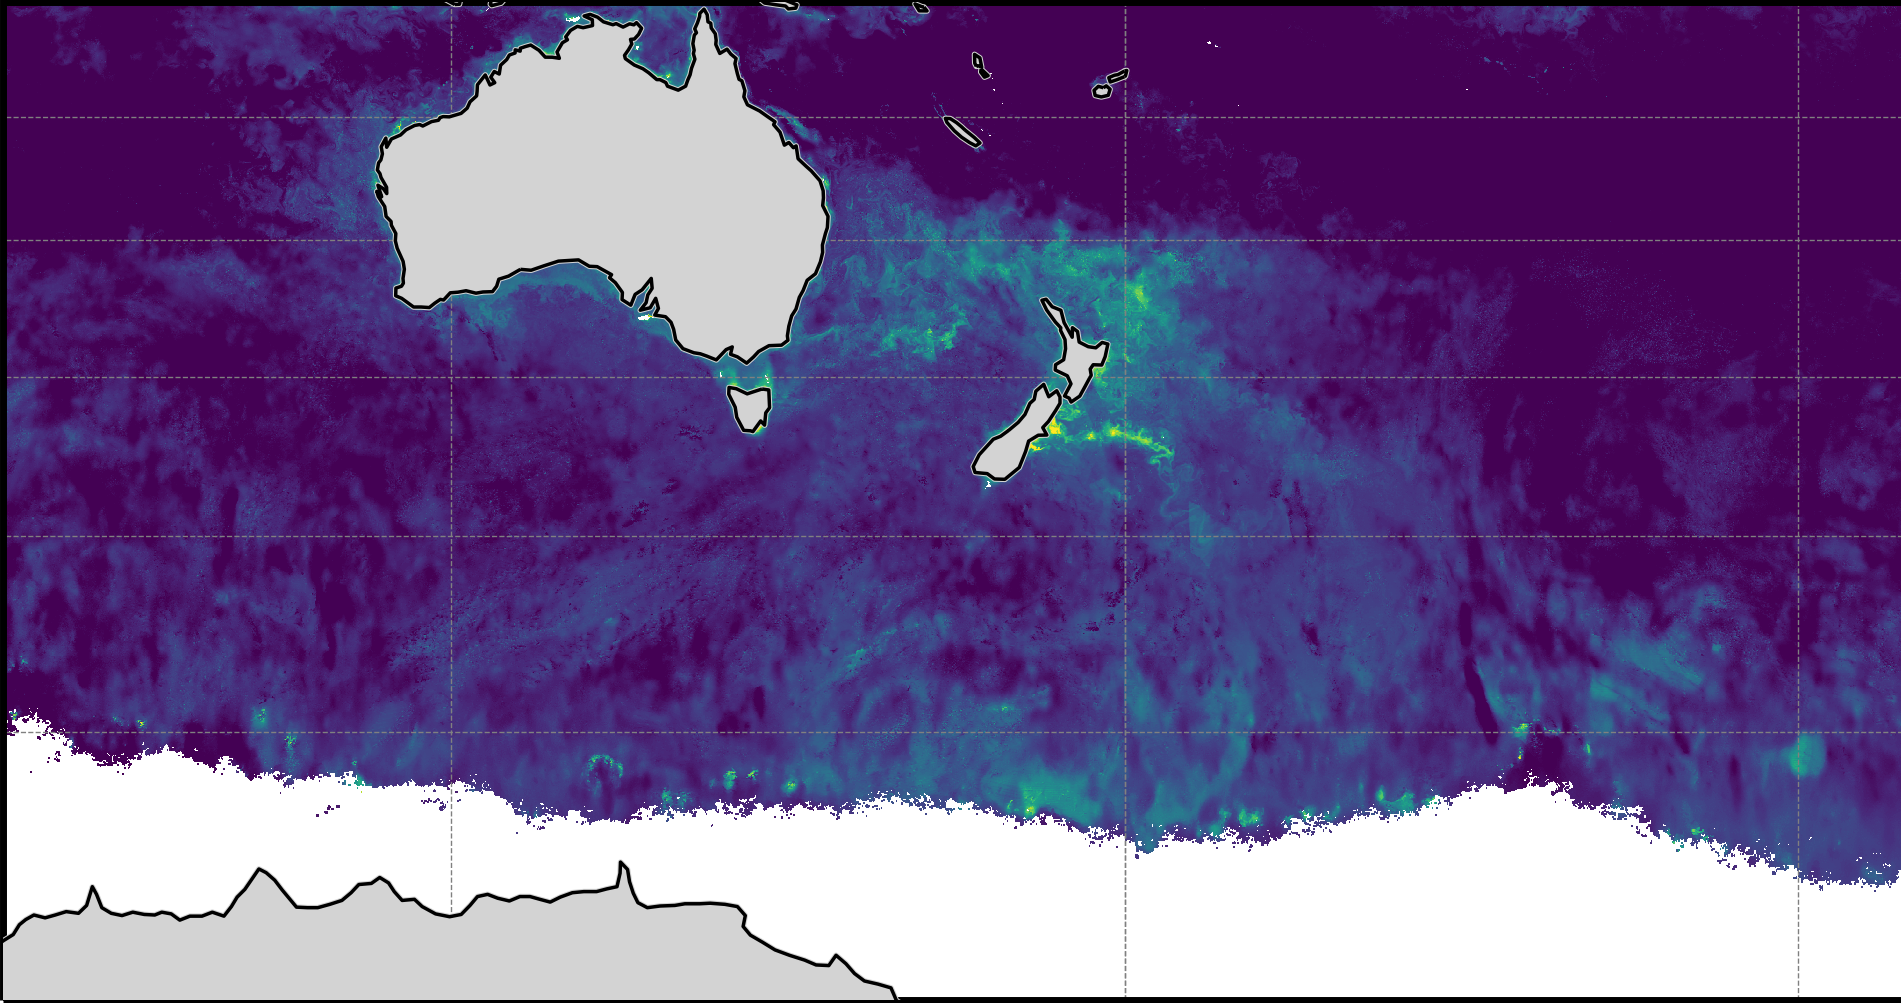
\includegraphics[width=\textwidth]{bilder/chla_interpol.png}
	\end{minipage}\hfill
	\caption{Beispielhaft die zum 01.09.2009 abgeleiteten Chlorophyll a Konzentrationen. Links: Ableitung auf Basis der Beobachtungsdaten (Ocean colour daily data des Climate Data Store). Für die weißen Flächen liegen keine Daten vor. Rechts: Mithilfe weiterer Algorithmen von \citet{Saulquin.2019} interpolierte Werte für eine vollständigere Abdeckung.} \label{fig:chla}
\end{figure}
\subsection{Statistische Methoden} \label{sec:stats}
Um den statistischen Zusammenhang zwischen Staub-/Eiseneintrag und den Entwicklungen des Phytoplanktons zu untersuchen, werden hier zwei verschiedene Verfahren angewendet. Zunächst wird anhand einer Zeitreihenanalyse der mittleren Konzentrationen des Phytoplanktons (Kapitel \ref{sec:timeseries}) überprüft, ob im Untersuchungszeitraum nach dem Staubsturm  anschaulich eine Veränderung beobachtet wird. Um das Ergebnis zu überprüfen und etwaige Besonderheiten zu entdecken, werden die Entwicklungen anschließend noch hinsichtlich der räumlichen Verteilung untersucht und Korrelationsanalysen für jeden Gitterpunkt durchgeführt.
\subsubsection{Zeitreihenanalyse} \label{sec:timeseries}
Für die Zeitreihenanalyse werden alle Gitterzellen betrachtet, für die von der WRF-Simulation ausreichend hoher Eiseneintrag simuliert wurde. Das heißt, es wird angenommen, dass eine Reaktion des Phytoplanktons nur möglich ist, wenn die \textit{normalen} Eisenkonzentrationen durch den Staubeintrag nennenswert erhöht werden. Auf Basis von Abbildung \ref{fig:nutrient_iron} wird angenommen, dass die \textit{normalen Konzentrationen} für den überwiegenden Teil der zu untersuchenden Region mindestens etwa 0.07 nM (Nanomolar bzw. Nanomol pro Liter) betragen. Darüber hinaus wird angenommen, dass der überwiegende Teil des neu eingetragenen Eisens in den oberen $z_0 = 10$m des Oberflächenwassers konsumiert wird. Mit  $M_{\text{Fe}} =  55.845$ g/mol Molmasse des Elements Eisen ergibt sich die vom Modell simulierte Erhöhung der Eisenkonzentrationen $\Delta C_\text{Fe}$ durch Integration des Eisenflusses $F_\text{Fe}$ über die Gesamtsimulationszeit:
\begin{equation}
\Delta C_\text{Fe} = \frac{1}{M_\text{Fe} \cdot z_0} \int F_\text{Fe} \cdot dt
\end{equation}
Um eine Erhöhung der Konzentrationen in der Größenordnung von $\Delta C_\text{Fe}=$0.01 nM zu erreichen, müssen dementsprechend wenigstens etwa $5.6$ µg Eisen pro Quadratmeter eingetragen werden. Zum Vergleich: In den \textit{Bottle Experiments} von \citet{Martin.1988} wurden in verschiedenen Behältern 1 nM, 5 nM und 10 nM hinzugefügt. Die Mengen waren dort also um mindestens zwei Größenordnungen höher als in dieser Annahme. Im SOIREE-Experiment für den südlichen Ozean \citep{Trull.2001} konnten Veränderungen ab einer Schwelle von etwa 0.2 nM Eisen beobachtet werden, was einer Verdopplung der dortigen regulären Konzentration von 0.1 nM entspricht \citep{Boyd.2010}. Auch im Vergleich dazu ist der hier verwendete Schwellenwert eher optimistisch, das heißt, die Ablagerungen reichen möglicherweise nicht aus, um eine Reaktion des Phytoplanktons zu bewirken. Da allerdings in einigen Regionen möglicherweise mehr Eisen eingetragen wurde, als vom Modell simuliert (insbesondere im Tasmanischen Meer, sh. Kapitel \ref{sec:wrf_results}), ist diese \textit{optimistische} Abschätzung bewusst gewählt. Die  chemischen Zusammensetzungen und Bedingungen sind für einzelne Regionen unterschiedlich (sh. Abb. \ref{fig:factors_collage}), weshalb die Domäne zwecks separater Analyse in verschiedene Sektoren eingeteilt wird. Für jeden Sektor wird anschließend für jeden verfügbaren Zeitpunkt der Mittelwert der Chlorophyll-a-Konzentrationen $\text{C}_{i,j}$ aus den $N$ dort betroffenen Zellen berechnet. Damit ergibt sich eine Zeitreihe für die durchschnittliche Entwicklung des Phytoplanktons im gesamten Sektor $\mu_C(t)$:
\begin{equation}
\mu_C(t) = \frac{1}{N}\sum\limits_{i,j=1}^{N} \text{C}_{i,j}(t)
\end{equation}
Die Entwicklung des Phytoplanktons unterliegt (auch im Tasmanischen Meer \citep{Tilburg.2002}) einem jahreszeitlichen Gang sowie weiteren externen Einflüssen, die eine hohe Variabilität aufweisen können (vgl. Kapitel \ref{sec:nährstoffe}). Da der jahreszeitliche Trend in den Klimadaten enthalten ist, kann die Zeitreihe im Untersuchungszeitraum 2009 um diesen Effekt bereinigt werden. Hierzu werden Datensätze des \textit{Marine Copernicus Service} verwendet, welche die nötigen täglichen Klimadaten bereits liefern. Neben dem Mittelwert der Chlorophyll-a-Konzentrationen des jeweiligen Tages für die Jahre 1998 bis 2018 kann außerdem aus der Standardabweichung und den 3\%- und 97\%-Perzentilen ($\sigma$,$q_{0.03}$,$q_{0.97}$,) die entsprechende Variabilität abgeleitet werden. Der Klima-Mittelwert $\text{C}_{[cli]i,j}$ eines jeden Gitterpunktes wird ebenfalls über den gesamten jeweiligen Sektor gemittelt. Dieser Klima-Mittelwert dient zur Entfernung eines möglichen Trends im zu untersuchenden Sektor, sodass ausschließlich die Abweichung/Anomalie $\Delta \mu(t)$ zur \textit{normalen} Entwicklung dargestellt wird:
\begin{equation}
\Delta \mu_C(t) = \mu_C(t) - \mu_{C[cli]}(t) \label{eq:cli_anomalie}
\end{equation} 
Im Fall eines düngenden Effektes der Eisendpositionen sollte diese bereinigte Zeitreihe nach dem Eintrag einen steigenden Trend aufweisen. Um einzuschätzen, ob die Abweichungen überhaupt relevant sind, werden diese mit der Standardabweichung sowie den 3\%- und 97\%-Perzentilen verglichen. Liegt die Anomalie unter der durch die Standardabweichung gegebenen Schwelle, ist ein Zusammenhang eher unwahrscheinlich, die Abweichungen könnten aus einer gewöhnlichen, staub-unabhängigen Variabilität resultieren. Liegen diese im Gegensatz deutlich darüber oder erreichen sogar das 97 \%-Perzentil, handelt es sich um sehr seltene Ereignisse (in 97\% der Fälle liegen die Konzentrationen/Abweichungen unter diesem Wert), bei denen ein externer Einfluss wahrscheinlich ist. Kann dieser in diesem Fall in einen zeitlichen Zusammenhang mit den Ablagerungen gebracht werden, wäre das ein deutliches Indiz für einen Einfluss eingetragenen Eisens. Sämtliche Werte des Klimadatensatzes liegen je Gitterzelle vor und es werden entsprechend für den jeweiligen Sektor die Mittelwerte der Standardabweichung $\mu_\sigma (t)$ und der 3\%- bzw. 97\%-Perzentile  $\mu_{q_{0.03}}(t)$, $\mu_{q_{0.97}}(t)$ gebildet. $\mu_{\Delta C}(t)$ ist der Mittelwert des für jeden Gitterpunkt geschätzten Fehlers $ \Delta C_i(t)$ der Chlorophyll-a-Konzentrationen $C_i(t)$ (in 2009).
\begin{figure}[htbp]
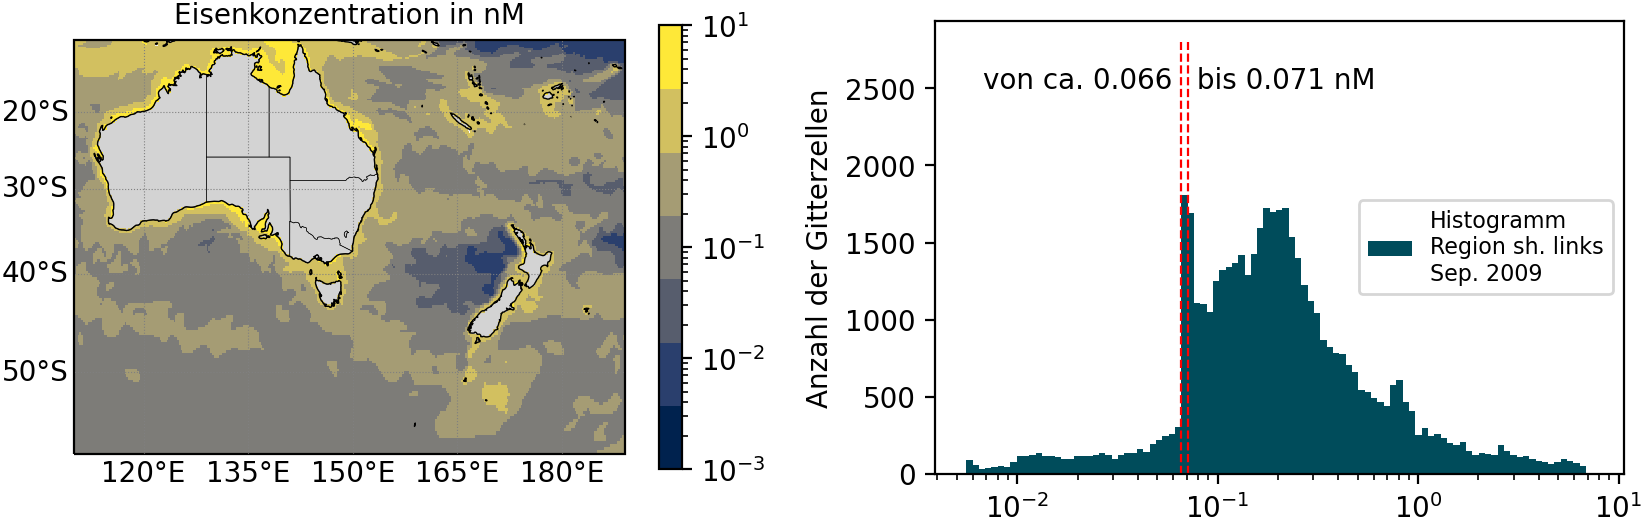
\includegraphics[width=\textwidth]{bilder/nutrient_iron.png}
\caption{Links: Die für September 2009 abgeleiteten Eisenkonzentrationen in der zu untersuchenden Region. Rechts: Histogramm für die Konzentrationen in den Gitterzellen. Für Informationen zur Datenquelle siehe Tabelle \ref{table:data}.} \label{fig:nutrient_iron}
\end{figure}
\subsubsection{Eisentransport durch Advektion} \label{sec:methods_advection}
Da dank der WRF-Simulation und den interpolierten Chlorophyll-a Daten \citep{Saulquin.2019} für die komplette Region räumlich vollständige Daten vorliegen, können diese Variablen neben dem zeitlichem Zusammenhang auch auf Muster untersucht werden. Im einfachsten Fall würden exakt die Regionen mit erhöhten Chlorophyll-Konzentrationen reagieren, in denen vorher Eisen eingetragen wurde. Im Rahmen dieser Arbeit wird vereinfacht angenommen, dass die Eisenpartikel ausreichend lange im Oberflächenwasser verweilen ($\approx$30 Tage, sh. auch \citet{Cropp.2013}), also nicht absinken und der Staubsturm grundsätzlich die einzige Eisenquelle bietet. Auch die weiteren begünstigenden oder abschwächenden Faktoren (Verfügbarkeit weiterer Nährstoffe, Wassertemperaturen, auf- und abströmen in (anti-)zyklonalen Wirbeln etc., Diffusion) werden mathematisch nicht berücksichtigt. Einzig der laterale Transport des eingetragenen Eisens aufgrund von Advektion soll berücksichtigt werden. Die Eisenkonzentrationen $C_\text{Fe}$ an einem Ort können sich gemäß der Kontinuitätsgleichung (\ref{eq:fe_continuity}) durch den Zu- oder Abfluss $\nabla . (C_\text{Fe} \vec{v})$ aufgrund der Ozeanströmung $\vec{v} = (u,v,w)^T$  und dem Eintrag eisenhaltigem Staubes $F_\text{Fe}$ verändern, welcher sich in der Wassersäule der Höhe $z_0$ gemäß der Annahme aus \ref{sec:timeseries} gleichmäßig verteilt:
\begin{equation}
\frac{\partial C_\text{Fe}}{\partial t} = - \nabla . (C_\text{Fe} \ \vec{v}) + \frac{1}{z_0 \cdot M_\text{Fe}} \cdot F_\text{Fe} \label{eq:fe_continuity}
\end{equation}
Da Ozeanwasser praktisch inkompressibel ist ($\nabla . \vec{v}=0$) und die Vertikalgeschwindigkeit $w\overset{!}{=}0$ vernachlässigt werden soll, reduziert sich der Ausdruck auf die zweidimensionale Advektionsgleichung:
\begin{equation}
\frac{\partial C_\text{Fe}}{\partial t} = - \vec{v} . \nabla_h  C_\text{Fe}  + \frac{1}{z_0 \cdot M_\text{Fe}} \cdot F_\text{Fe} \label{eq:fe_advection}
\end{equation}
Diese wird nach dem Upwind-Schema diskretisiert, sodass sich anschließend die Eisenkonzentrationen am Gitterpunkt $i,j$ für die Zeitschritte $n$ mit $\Delta t$= 3 Stunden ergeben:
\begin{equation}
\begin{split}
C_{i,j}^n = &\ C_{i,j}^{n-1} - u_{i,j}^{n-1} \cdot \frac{\Delta t}{\Delta x_{i,j}} \cdot (C_{i,j}^{n-1} - C_{i,j-1}^{n-1}) \\\\
&- v_{i,j}^{n-1} \cdot \frac{\Delta t}{\Delta y_{i,j}} \cdot (C_{i,j}^{n-1} - C_{i-1,j}^{n-1})  \\\\
&+ \frac{\Delta t}{z_0 \cdot M_\text{Fe}} \cdot F_\text{Fe} \text{ \qquad  \qquad \qquad für } u,v > 0
\end{split}
\end{equation}
Die Courant-Zahl $c = u \cdot \Delta t / \Delta x$ bzw. $v \cdot \Delta t / \Delta y$ bleibt in diesem Fall bei den minimalen Gitterpunktabständen von knapp 30km (sh. Kapitel \ref{sec:wrf}) für Strömungskomponenten $u,v \ < 2.6$ (hier überall gegeben) kleiner als 1, sodass das Schema gemäß der \textit{Courant-Friedrich-Lewy}-Bedingung stabil bleibt. Die Strömungsgeschwindigkeit auf den Landflächen beträgt Null. Als Randbedingungen werden die Eisenkonzentrationen auf Landflächen ebenfalls gleich Null gesetzt. Dadurch werden an den Küstengitterpunkten die Konzentrationen zwar bei entsprechenden Strömungen (bei denen die Komponente normal zur Küste ungleich Null ist) künstlich verringert. Da die Einträge in Küstennähe ohnehin relativ hoch sind (sh. Kapitel \ref{sec:wrf_results}) und die Berechnung nur der qualitativen Abschätzung dient, wird dieser Fehler jedoch zugunsten der Stabilität, einfachen Implementierung und kurzen Rechenzeit akzeptiert.
\subsubsection{Korrelationsanalyse} \label{sec:methods_correlation}
Um einen räumlichen Zusammenhang zwischen den Veränderungen der Eisenkonzentrationen $\partial C_\text{Fe} / \partial t$ und den Veränderungen in den Chlorophyll-a-Konzentrationen $\partial C / \partial t$ zu untersuchen, wird eine Korrelationsanalyse beider Zeitreihen durchgeführt. Ebenso wie die Eisenkonzentrationen können sich die Chlorophyll-a-Konzentrationen an einem Ort gemäß der Kontinuitätsgleichung \ref{eq:continuity} nur durch Zu-/Abfluss und aufgrund möglicher Senken/Quellen $S_C$ ändern.
\begin{equation}
\frac{\partial C}{\partial t} = - \nabla . (C \ \vec{v}) + S_C  \overset{\text{inkompressibel}}{=} - \vec{v}.\nabla C + S_C \label{eq:continuity}
\end{equation}
Im Rahmen der Analyse wird der Fluss $\vec{v}.\nabla C$ hier jedoch vernachlässigt, sodass die Veränderungen ausschließlich auf die mögliche Quelle (Wachstum nach Düngung durch zusätzlich verfügbarem Eisen) mit einer (hier unbekannten) Wachstumsfunktion $S_C = f(\partial C_\text{Fe} / \partial t)$ zurückgeführt werden. Falls ein (näherungsweise) linearer Zusammenhang besteht, hängt die Entwicklung der Chlorophyll-a-Konzentrationen dann direkt proportional von den verfügbaren bzw. veränderten Eisenkonzentrationen ab, sodass dieser Zusammenhang im Rahmen einer Korrelationsanalyse sichtbar werden sollte. Im ersten Schritt werden die Koordinaten (d.h. die Gitterpunkte) der Chlorophyll-a-Daten auf die des Eisenflusses aus der WRF-Simulation angepasst. Anschließend werden nach dem expliziten Euler-Rückwärts-Verfahren die Ableitungen für die täglichen Chlorophyll-a-Daten ($\Delta t = 1d$) berechnet:
\begin{equation}
\left[\frac{\partial C}{\partial t}\right]_{i,j}^{n} \approx \frac{C_{i,j}^n-C_{i,j}^{n-1}}{\Delta t}
\end{equation}
Danach werden für jeden Gitterpunkt die Kreuzkorrelationen für verschiedene Zeit- ($\tau$ in Tagen) und Gitterpunkt- ($\Delta i$,$\Delta j \in \mathbb{Z}$) Verschiebungen bestimmt:
\begin{equation}
R_{i,j}(\tau,\Delta i, \Delta j)= \frac{1}{N_t}\sum\limits_{n=1}^{N_t} \left[\frac{\partial C_\text{Fe}}{\partial t}\right]_{i,j}^n \cdot \left[\frac{\partial C}{\partial t}\right]_{i+\Delta i ,j+\Delta j}^{n+\tau}
\end{equation}
Daraus können noch durch Subtraktion der Zeitmittelwerte die Kovarianz (\ref{eq:covariance}) und der durch Normierung um die zeitlichen Standardabweichung auf das Intervall $[-1,1]$ beschränkte Korrelationskoeffizient $\rho_{i,j}(\tau,\Delta i, \Delta j)$ berechnet werden (\ref{eq:corrcoeff}):
\begin{equation}
\text{cov}_{i,j}(\tau,\Delta i, \Delta j) = R_{i,j}(\tau,\Delta i, \Delta j)-\left[\frac{\overline{\partial C_\text{Fe}}}{\partial t}\right]_{i,j} \cdot \left[\frac{\overline{\partial C}}{\partial t}\right]_{i+\Delta i,j+\Delta j}^{+\tau} \label{eq:covariance}
\end{equation}
\begin{equation}
\rho_{i,j}(\tau,\Delta i, \Delta j) = \frac{\text{cov}_{i,j}(\tau,\Delta i, \Delta j)}{\sigma \left(\left[\frac{\partial C_\text{Fe}}{\partial t}\right]_{i,j}\right) \cdot \sigma\left(\left[\frac{\partial C}{\partial t}\right]_{i+\Delta i ,j+\Delta j}^{+\tau}\right)} \label{eq:corrcoeff}
\end{equation}
Um die Aussagekraft des Korrelationskoeffizienten $\rho$ zu bestimmen, wird der P-Wert bzw. zweiseitige t-Test verwendet. Der P-Wert gibt die Wahrscheinlichkeit an, mit welcher der berechnete Korrelationskoeffizient auf Basis der Daten (mit angenommener t-Verteilung) erreicht werden könnte, wenn eigentlich keine Korrelation vorliegt, in der Realität also $\rho=0$ gälte (Nullhypothese). Er trifft damit Aussagen über die Signifikanz des Ergebnisses. Da die Anzahlen der Beobachtungen $N$ und Freiheitsgrade $N-2$ bei der späteren Auswertung hier immer gleich bleiben, kann direkt der Mindestwert berechnet werden, den der Korrelationskoeffizient erreichen muss, um signifikant zu sein. Für ein Signifikanzniveau vom 95\% bei $N = 12$ Beobachtungen ist $t_{0.975}\approx 2.2$, sodass:
\begin{equation}
t = \frac{\rho \cdot \sqrt{N-2}}{\sqrt{1-\rho^2}} \Leftrightarrow \rho = \sqrt{\frac{1}{\frac{N-2}{t}+1}} \Rightarrow |\rho| \geq 0.57 
\end{equation}
Unter idealen Bedingungen sollten die Korrelationen bei einer Zeitverschiebung $\tau$ maximal sein, die genau der Reaktionszeit des Phytoplanktons entspricht. Die räumliche Verschiebung um $\Delta i$ und $\Delta j$ kann als Alternative zu dem mit der Advektionsgleichung berechneten Eisentransport (sh. \ref{sec:methods_advection}) angewendet werden. Um $\Delta i$ und $\Delta j$ sinnvoll zu bestimmen, wird die potentielle Verschiebung eines jeden Gitterpunkts vom ursprünglichen Ort $\vec{x}_{i,j}(0)$ (Ort des Eiseneintrags) durch die Strömung nach entsprechender Zeitverschiebung $\tau \in \mathbb{N}_0$ berechnet:
\begin{equation}
\frac{\partial \vec{x}}{\partial t} = \vec{v}(\vec{x},t) \Rightarrow \vec{x}_{i,j}(\tau) =   \vec{x}_{i,j}(0) + \Delta t \cdot \sum\limits_{n = 1}^{\tau} \vec{v} \left( \vec{x}(\tau - n \cdot \Delta t),\tau - n \cdot \Delta t \right) \label{eq:position_shift}
\end{equation}
\section{Ergebnisse und Diskussion} \label{sec:auswertung}
In diesem Kapitel werden die Ergebnisse der WRF-Simulation verwendet, um den potentiell düngenden Effekt der Staubereignisse Ende September 2009 auf die Phytoplankton-Populationen zu untersuchen. Die Analyse mündet in drei wesentliche Ergebnisse:
\begin{enumerate}
\item Es können erhöhte Chlorophyll-Konzentrationen nach dem Staubeintrag festgestellt werden.
\item Die Regionen mit Staubniederschlägen stimmen zum Teil räumlich mit denen erhöhter Chlorophyll-Konzentrationen überein.
\item Eine Reaktion tritt je Region nach unterschiedlichen Zeiten ein.
\end{enumerate}
Zuerst werden hierzu die Ergebnisse der Simulation präsentiert, um die Ausmaße des modellierten Staubsturms zu quantifizieren. 
\subsection{Ergebnisse der WRF-Simulation} \label{sec:wrf_results}
Auf Abbildung \ref{fig:dustload} werden die Ausdehnung der Staubwolke und die Quellen täglich um 0 Uhr UTC präsentiert. Es ist erkennbar, dass sich die Staubkonzentrationen auch über das Untersuchungsgebiet hinaus erstrecken. Die Staubwolke stimmt in Ausmaß und Form gut mit den Beobachtungen aus den Satellitenbildern (Abb. \ref{fig:satellite}) überein. Es sind alle Hauptereignisse (gem. \cite{Leys.2009}) identifizierbar: Das Ereignis beginnt mit hohen Staubkonzentrationen über Canberra am 22.09., zeigt am 23.09. um 0 Uhr UTC zum Zeitpunkt des Red Dawn die sehr hohen Konzentrationen entlang der gesamten West-Nordwest-Küste, und auch der kleinere \textit{Folgesturm} am 26.09. ist deutlich abgebildet. Ab dem 24.09. simuliert das WRF-Modell sehr hohe Staubkonzentrationen im Norden und Nordwesten Australiens. Diese sind anhand der Satellitenbilder nicht eindeutig ableitbar. Darüber hinaus suggerieren die Satellitenbilder (Abb. \ref{fig:satellite} B), dass die höheren bzw. maximalen Konzentrationen innerhalb der Staubwolke vom 23. September verglichen mit der WRF-Simulation etwas südlicher waren, mit besonders hoher Dichte in der Region um und nördlich von Sydney. Dieser Eindruck korrespondiert mit den direkten Beobachtungen und PM10-Messungen (partikelförmige Materie kleiner als 10µm, \cite{Leys.2011}). Aus den Bodenmessungen ergeben sich PM10-Konzentrationen von maximal 15 366 µg/m3 in Bringelly und Konzentrationen über 10 000 µg/m3 direkt in Sydney (Newcastle, Randwick). Tatsächlich simuliert das WRF-Modell in dieser Region (150-152°E, 33-35°S) zu dieser Zeit (Maximum am 23.09. 0 Uhr UTC) für die Bodenschicht (geländefolgend, 55-57 m dick) deutlich schwächere mittlere Konzentrationen um maximal 4 µg/m3. Erst nördlich kurz unterhalb der Grenze von New South Wales und Queensland ab etwa 30°S werden Konzentrationen von mehr als 450 µg/m3 simuliert, die immerhin die Anforderungen an eine \textit{mäßige Trübung} (vgl. \cite{Leys.2011}) erfüllen. Maximale Bodenkonzentrationen von 14 713 µg/m3 treten lediglich am 22.09. um 15 Uhr UTC direkt an einer Quelle in Channel Country (s.u.) auf. Das bedeutet, dass das namensgebende \textit{Red Dawn Event} in Sydney durch die Simulation lokal nur schlecht reproduziert wird. Nichtsdestotrotz deckt sich die grundsätzliche Ausdehnung der Staubwolke aufgrund der logarithmischen Skalierung in Abb. \ref{fig:dustload} gut mit den Satellitenbildern, sodass eine weitere Analyse qualitativ möglich ist. Angesichts der Trajektorie der Staubwolke in Abb. \ref{fig:dustload} ist jedoch zu berücksichtigen, dass die absoluten Werte der Konzentrationen (und später Einträge) östlich von New South Wales und im Süden möglicherweise deutlich höher lagen, als durch das Modell simuliert. \citet{AlizadehChoobari.2012} erhielten ähnliche Abweichungen, in denen die simulierten Werte der Aeorsol Optischen Tiefe (AOD) über dem Tasmanischen Meer geringer und im Nordwesten Australiens deutlich höher waren als die Satellitenaufnahmen anzeigen. Deren Simulation erreicht mit 1876 µg/m3 immerhin signifikant erhöhte PM10-Konzentrationen im Raum Sydney (Vineyard, gemessen wurden 11 174 µg/m3). Die deutlichen Abweichungen können hier, als auch bei \citet{AlizadehChoobari.2012} aus einer Unterschätzung möglicher lokaler Staubquellen in New South Wales resultieren (sh. Kapitel \ref{sec:reddawn}), die in der hier präsentierten Simulation keine Emissionen generierten.
\begin{figure}[htbp]
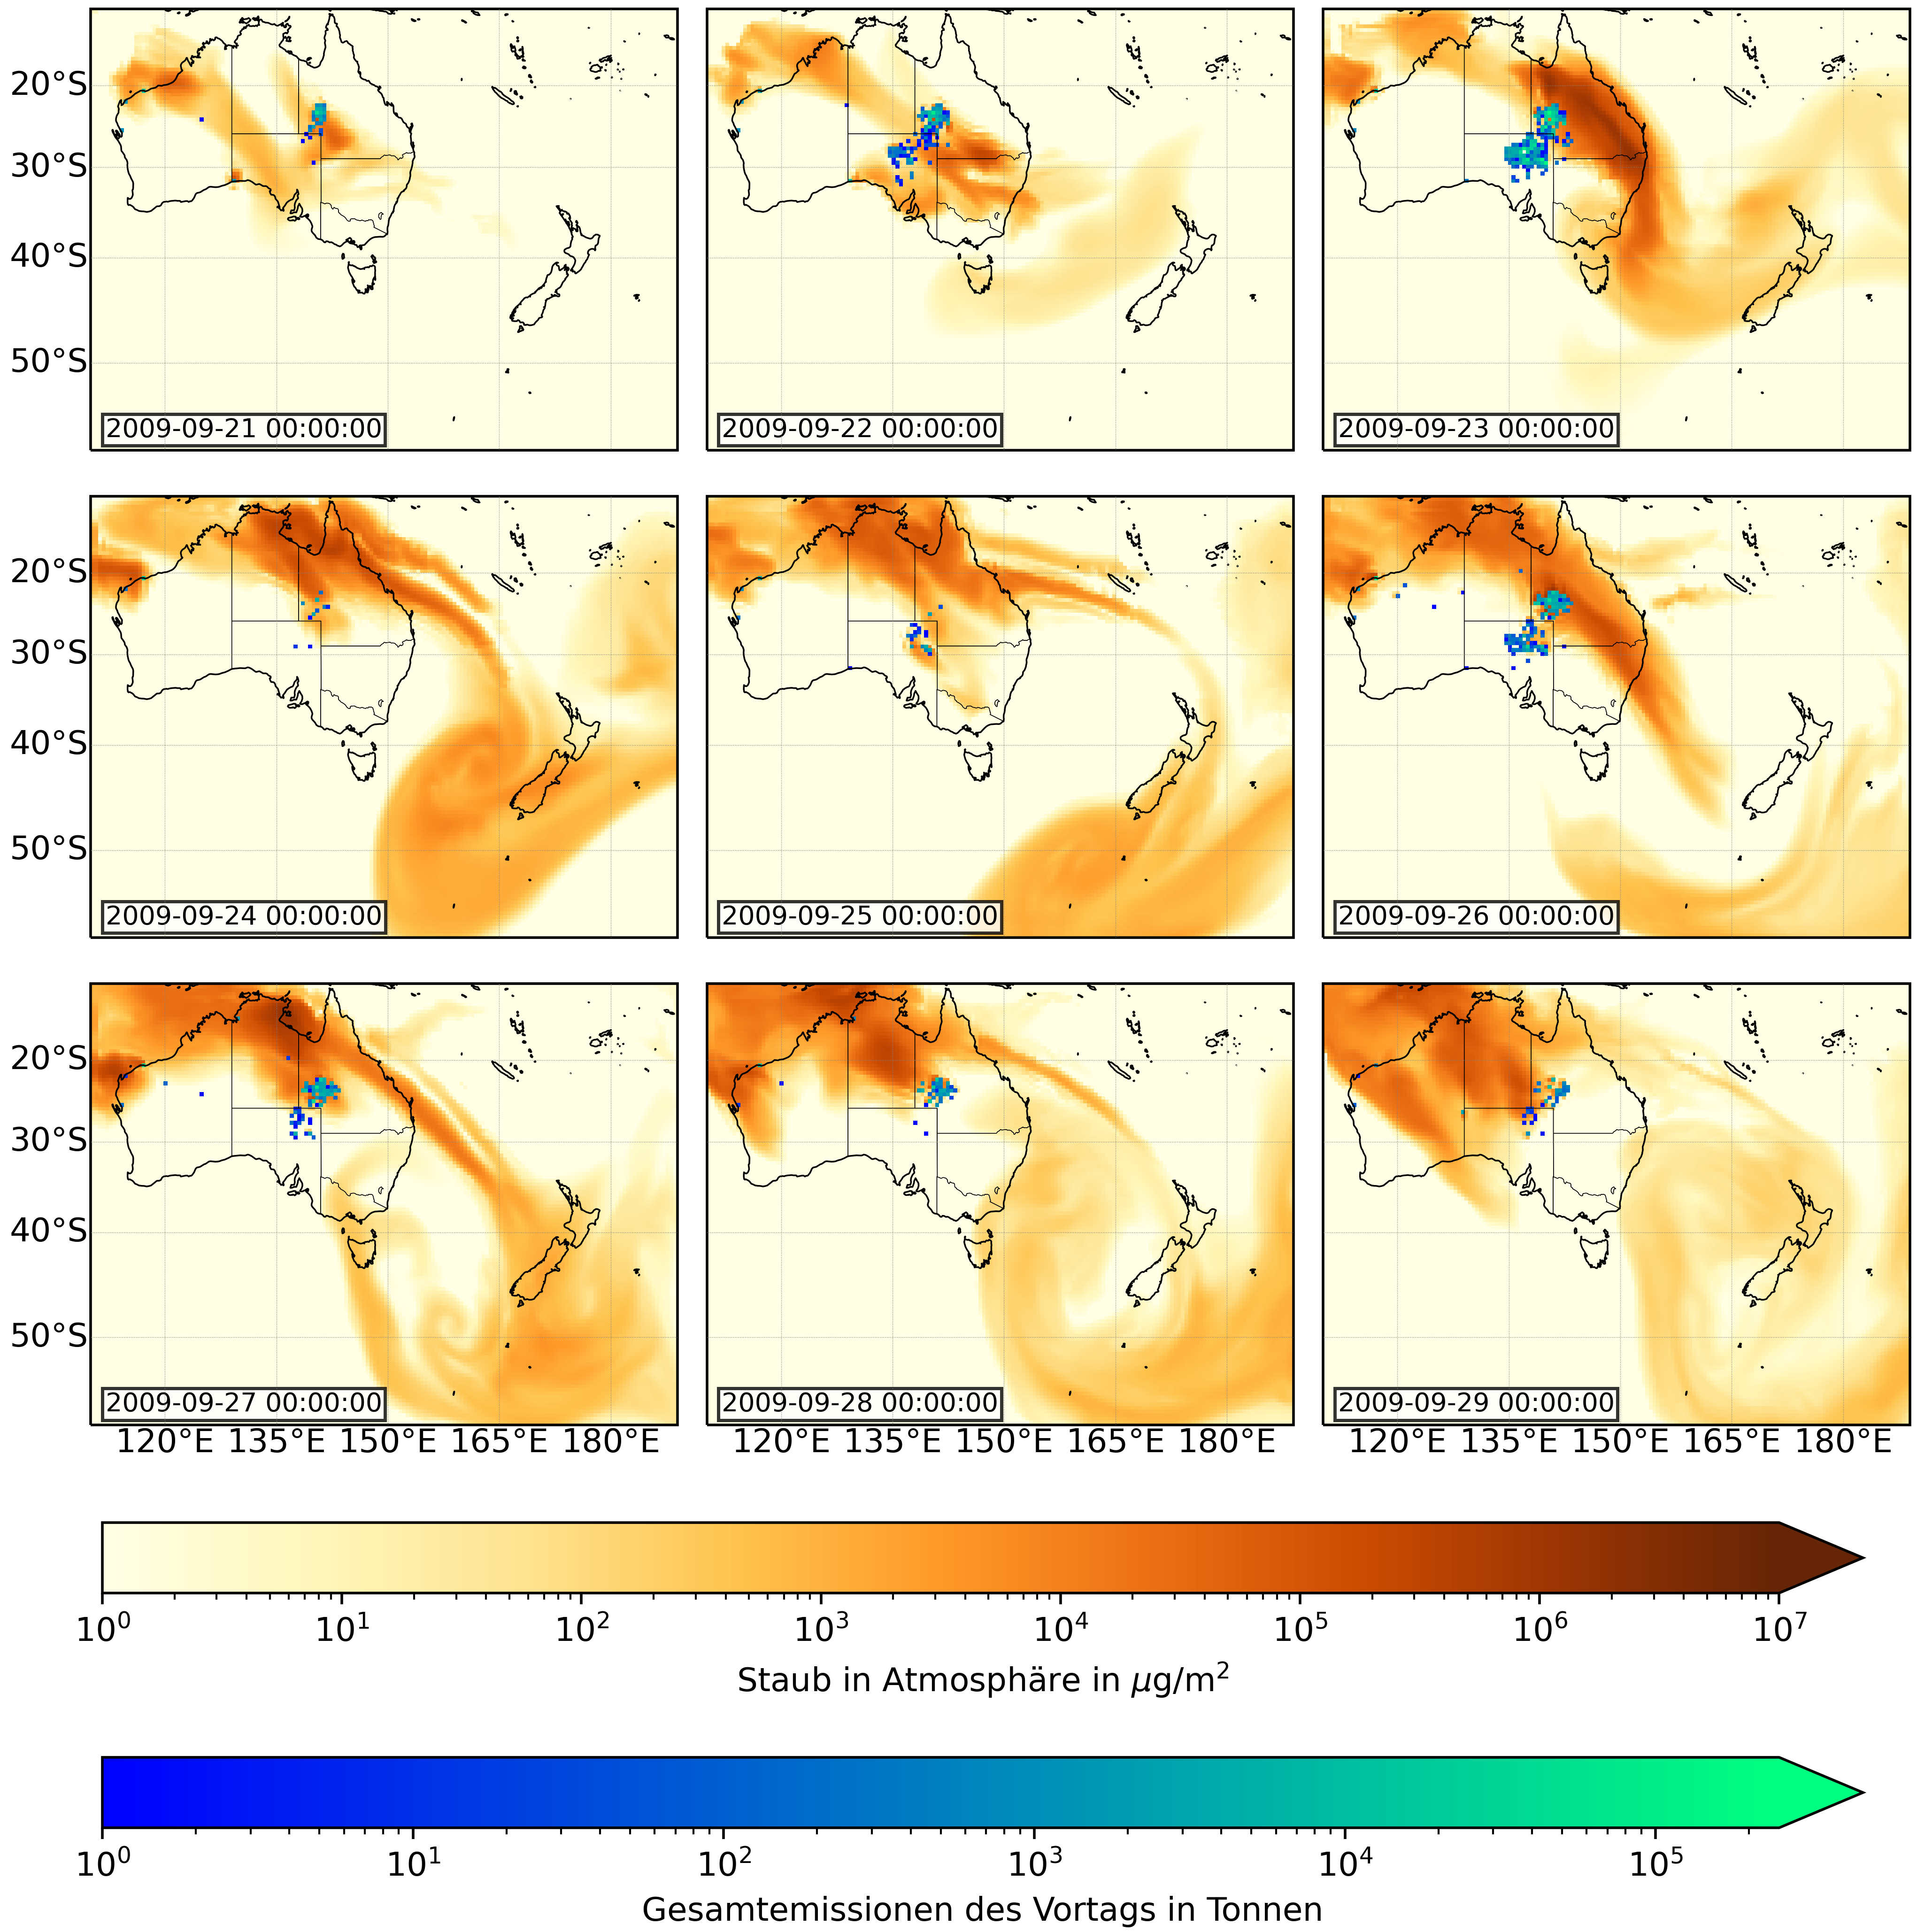
\includegraphics[width=\textwidth]{bilder/dustload.png}
\caption{Anschauliche Darstellung der durch das WRF-Modell simulierten Ausdehnung der Staubwolke und der Emissionsquellen für die 9 Tage mit nennenswerten Bewegungen zu 0 Uhr UTC. Jeweils unten links in der Box sind die bis zum genannten Zeitpunkt kumulierten Tages-Emissionen in Tonnen ausgegeben. Der mit Abstand größte Teil (1974 tausend Tonnen bzw. knapp 2Tg) wird demnach am 22. September emittiert. } \label{fig:dustload}
\end{figure}
Die Simulation präsentiert zwei Regionen, welche die wesentlichen Hauptquellen darstellen: 1) \textit{Channel Country} im Westen von Queensland und 2) große Teile des Lake Eyre Beckens in Südaustralien, siehe Abbildung \ref{fig:emissions}. Knapp zwei Drittel stammen aus der Region Channel Country, etwa ein Drittel aus dem etwas südlicheren Teil des Lake Eyre Beckens. Beide Quellen wurden in vorangegangenen Arbeiten ebenfalls identifiziert (sh. Kapitel \ref{sec:reddawn}). Die weiteren mutmaßlichen Quellen (Bergbaugebiete um Cobar und Broken Hill und Weideland im Nordwesten von New South Wales) spielen in der Simulation allerdings  keine Rolle. Wie oben angemerkt, könnte dies eine Schwachstelle der Simulation darstellen. Darüber hinaus wird der Großteil des Staubes von nur einigen wenigen Gitterzellen emittiert. Die Gesamtemission beträgt 3.4 Millionen Tonnen (= 3.4 Tg, davon 2.3 Tg bis zum 23.09. um 0 Uhr UTC). Davon werden allein 650 tausend Tonnen, also etwa 19 \% von nur einer Zelle in Channel Country abgetragen, welche eine Landfläche der Größe von knapp 2500 Quadratkilometern repräsentiert. Im Modell wird die Landfläche Australiens durch 3226 Gitterpunkte abgebildet. Davon emittieren 195 Staub, wovon wiederum nur 6 fast die Hälfte (48.9 \%) der Gesamtemissionen ausmachen. 75 \% werden bereits von 20 Quellen repräsentiert, 42 sind für über 90 \% verantwortlich, sh. Abbildung \ref{fig:emissions}. 
\begin{figure}[htbp]
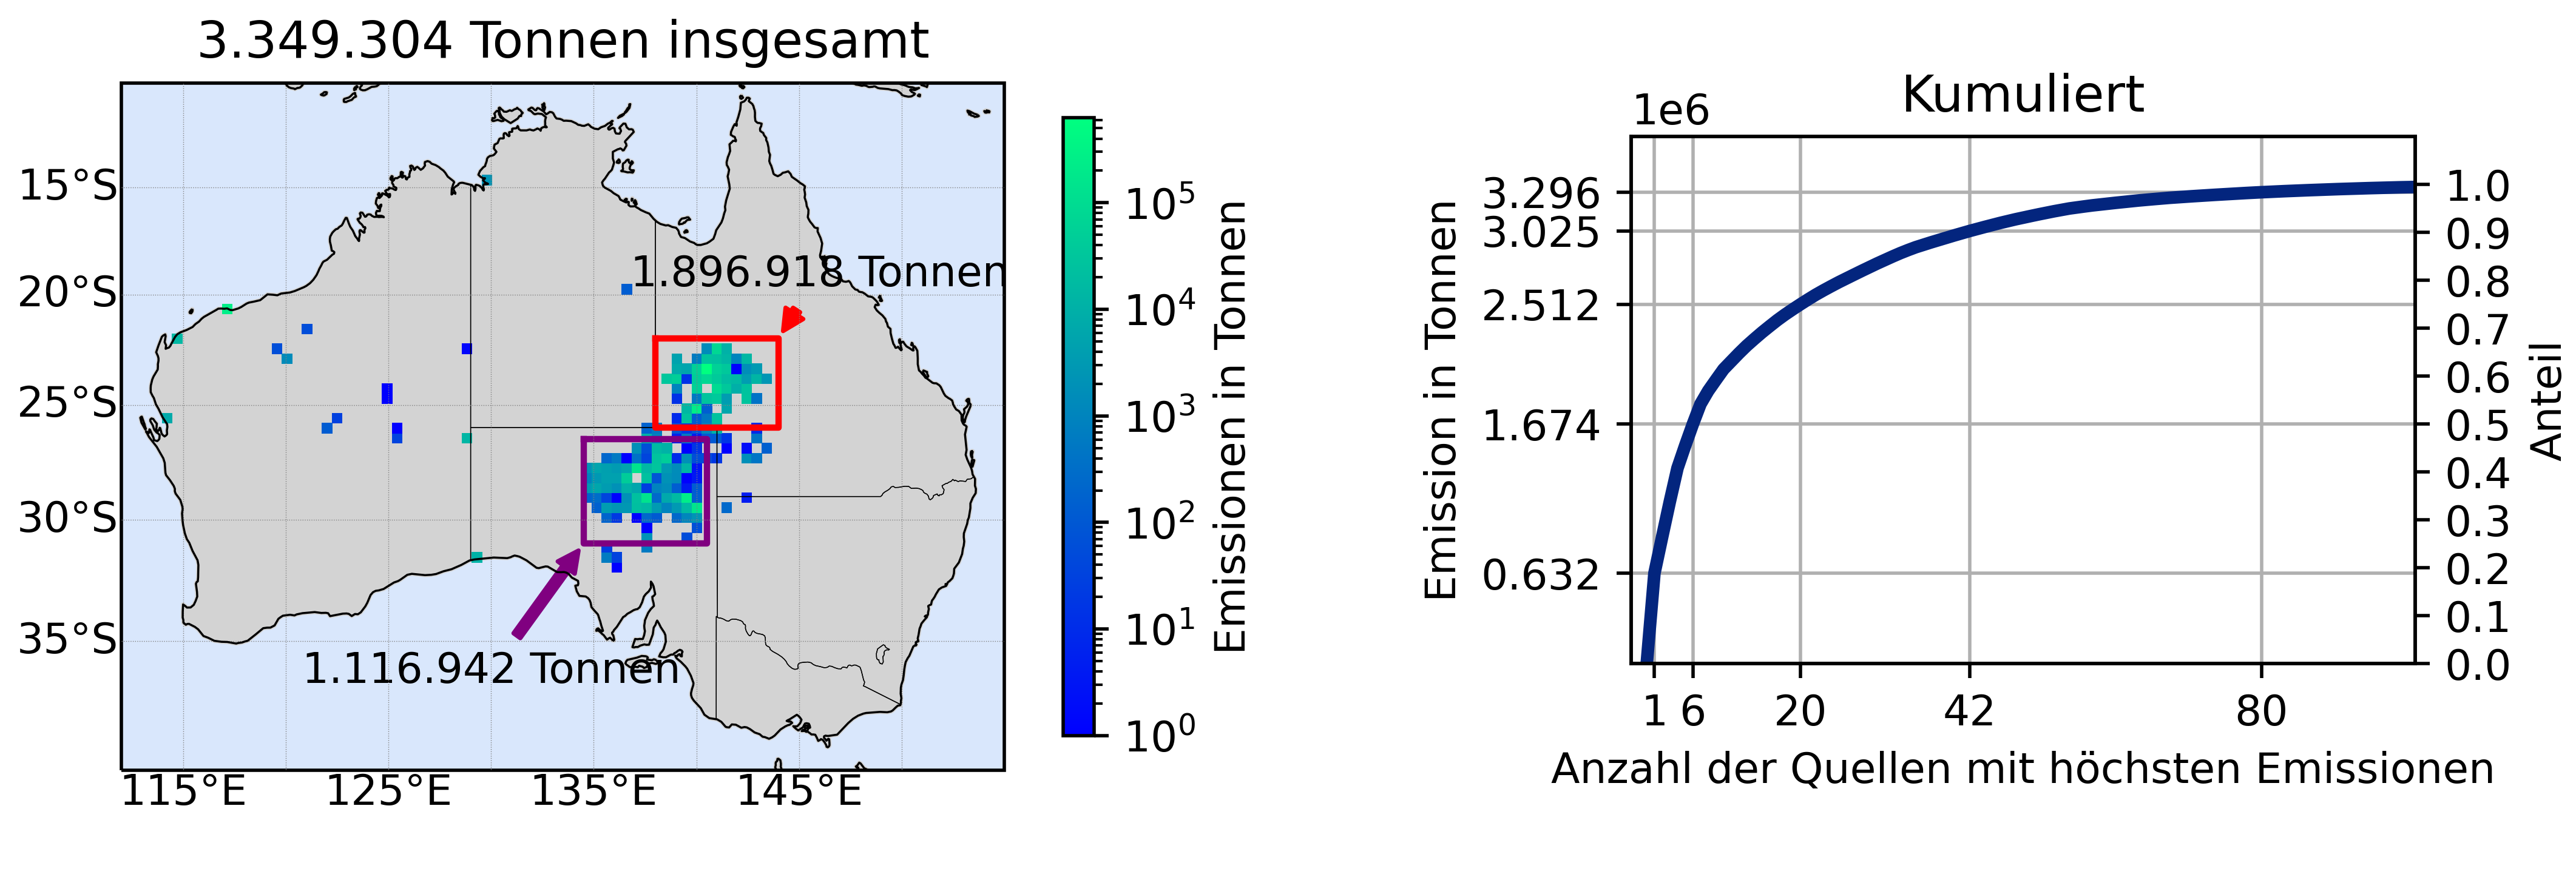
\includegraphics[width=\textwidth]{bilder/emission_sections.png}
\caption{Links: Darstellung der Staubquellen und Gesamtemissionen je Gitterpunkt. Es werden grob zwei Hauptregionen identifiziert: Channel Country (roter Kasten) und das Lake Eyre Becken in Südaustralien (violetter Kasten). Rechts: Darstellung der Abhängigkeit von einzelnen Quellen. Die logarithmisch ansteigende Kurve zeigt, dass wenige Gitterpunkte einen Großteil der Emissionen beschreiben.} \label{fig:emissions}
\end{figure}
Die Staubwolke erreicht ca. am 22. September um 9 Uhr UTC mit knapp 1.2 Tg ihre maximale Beladung, siehe Abbildung \ref{fig:dustload_time}. Über die Hälfte des Staubs wird noch am 23. September wieder auf Land- und Ozeanflächen eingetragen. Durch zusätzliche Emissionen am 28. September halten die maximalen Staubkonzentrationen beim zweiten Hauptereignis ab dem 26.09. etwas länger an, die absoluten Werte liegen aber etwa bei der Hälfte des größeren Ereignisses vom 23. September. Zum Ende der Simulation befinden sich noch etwa 0.2 Tg Staub in der Atmosphäre (d.h., ohne Berücksichtigung des Teils außerhalb des Untersuchungsgebietes).
\begin{figure}[htbp]
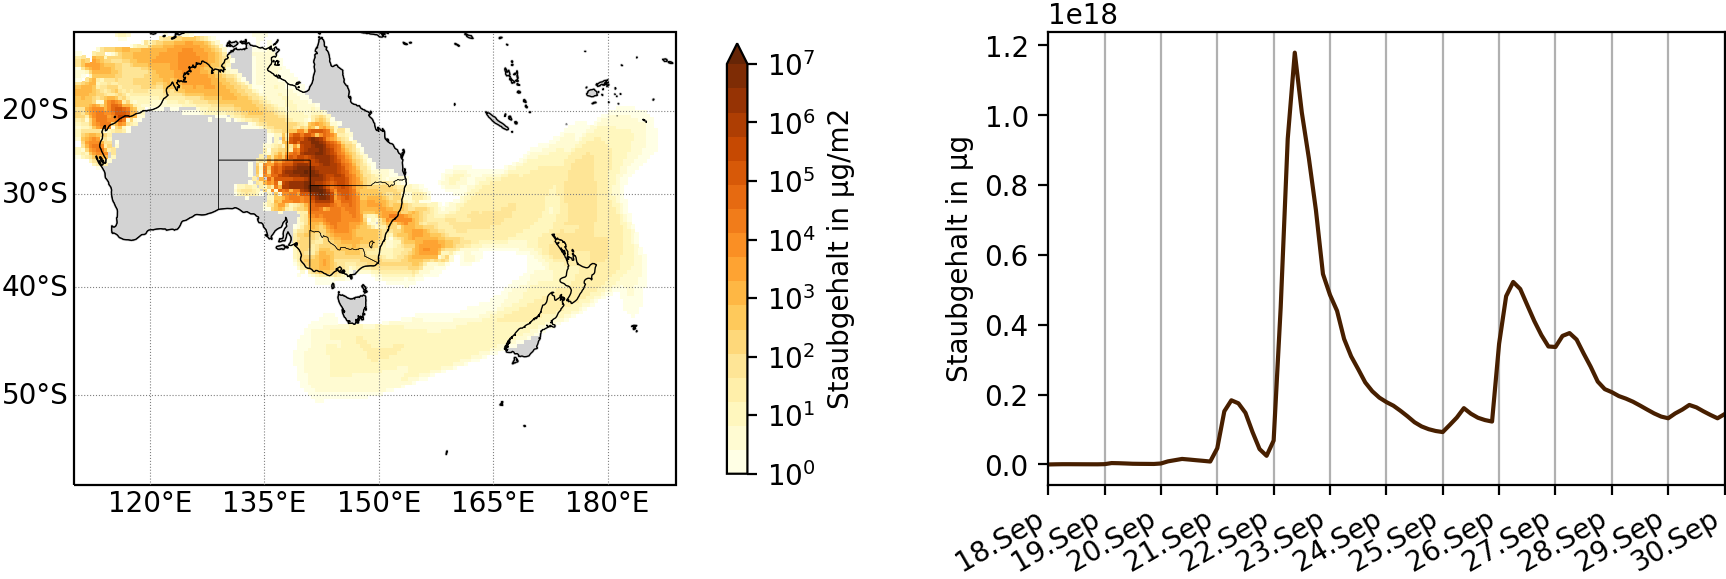
\includegraphics[width=\textwidth]{bilder/dustload_time.png}
\caption{Links: Maximale Beladung der Staubwolke am 22. September um 9 Uhr UTC. Rechts: Zeitserie des Staubgehaltes in der Atmosphäre für den kompletten Simulationszeitraum} \label{fig:dustload_time}
\end{figure}
Von den etwa 3.4 Tg Staubemissionen werden innerhalb des WRF-Simulationszeitraums etwa 1.7 Tg wieder auf den betrachteten Land- und Ozeanflächen eingetragen. Abbildung \ref{fig:deposition} zeigt, dass der Großteil des Staubs laut Modell in direkter Nähe zur Quelle trocken wieder eingetragen wird. Nur ein geringer Teil erreicht tatsächlich den Ozean der hier betrachteten Domäne, ein großer Teil wird nördlich und westlich außerhalb abtransportiert. 
\begin{figure}[htbp]
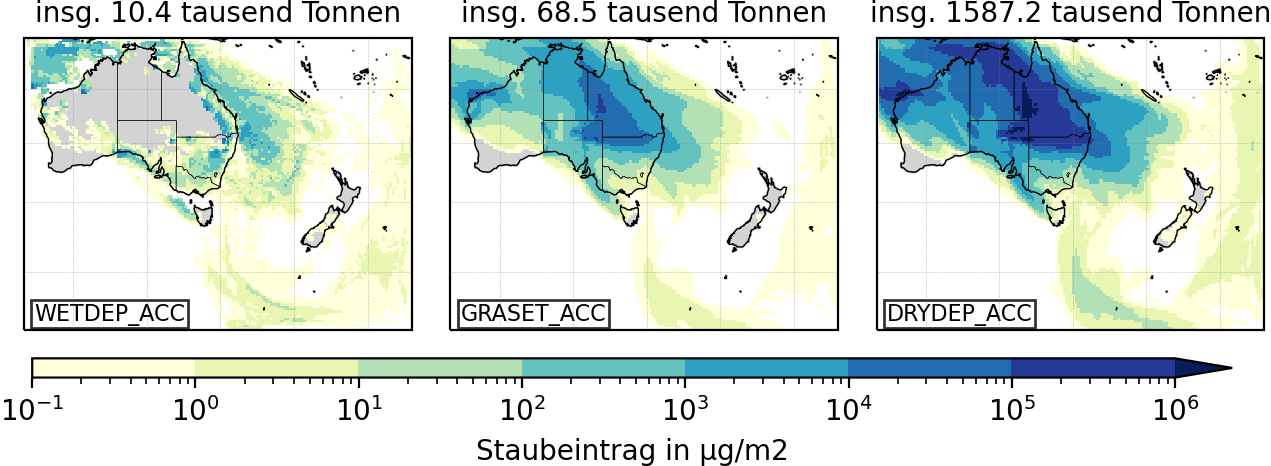
\includegraphics[width=\textwidth]{bilder/dust_deposition_vars.png}
\caption{Kumulierter Eintrag von Staub über den gesamten Simulationszeitraum. Der Gesamteintrag ergibt sich als Summe von nassem Eintrag (links, Auswaschung durch Regen), Ablagerung durch Gravitation (Mitte) und trockenem Staubeintrag (rechts).} \label{fig:deposition}
\end{figure}
Ein ähnliches Muster zeigt sich bei den darin enthalten Eisenniederschlägen (Abb. \ref{fig:iron_deposition}). Insgesamt werden lt. Simulation knapp 19 tausend Tonnen (0.019 Tg) Eisen eingetragen. Wesentlicher Unterschied ist allerdings, dass hier der Eintrag aufgrund der Erdbeschleunigung (\textit{gravitional settling}) dominiert.  In beiden Fällen erreicht nur ein sehr kleiner Bruchteil den für die Eisenhypothese wichtigen südlichen Ozean.
\begin{figure}[htbp]
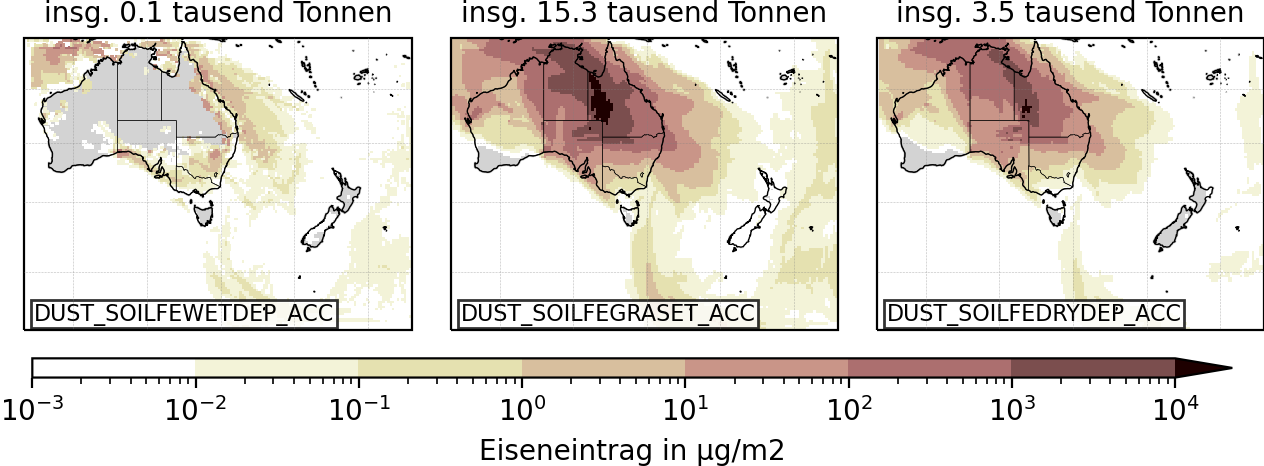
\includegraphics[width=\textwidth]{bilder/iron_deposition_vars.png}
\caption{Kumulierter Eintrag von Eisen über den gesamten Simulationszeitraum. Der Gesamteintrag ergibt sich als Summe von nassem Eintrag (links, Auswaschung durch Regen), Ablagerung durch Gravitation (Mitte) und trockenem Staubeintrag (rechts).} \label{fig:iron_deposition}
\end{figure}
Im folgenden wird der Eiseneintrag genauer analysiert. Hierzu wird die Domäne in 5 Regionen unterteilt. In Abbildung \ref{fig:iron_deposition_sections} ist das räumliche Muster der Eiseneinträge mit den zugehörigen Zeitserien dargestellt. Zeitpunkt und Höhe des Eintrags unterscheiden sich je nach Region deutlich. Insgesamt werden etwas über 2.000 Tonnen, also knapp 11 \% der Gesamtablagerungen in den Ozean eingetragen, davon der überwiegende Teil mit knapp 1.900 Tonnen im Nordwesten am 26. und 27. September. Weniger als ein Zehntel davon wird lt. WRF-Modell in das Korallenmeer und das Tasmanische Meer eingetragen. Diese Eisen-Niederschläge ereignen sich wenige Stunden nach dem Red Dawn am 23. September. In den Süden und den Südozean wird vergleichsweise wenig eingetragen. Wie in der Zeitreihe auf Abb. \ref{fig:iron_deposition_sections} zu sehen, wird ein Teil des Staubs scheinbar erst nach dem Simulationszeitraum eingetragen, da weiterhin Staub in der Atmosphäre ist (vgl. Abb. \ref{fig:dustload_time}).
\begin{figure}[htbp]
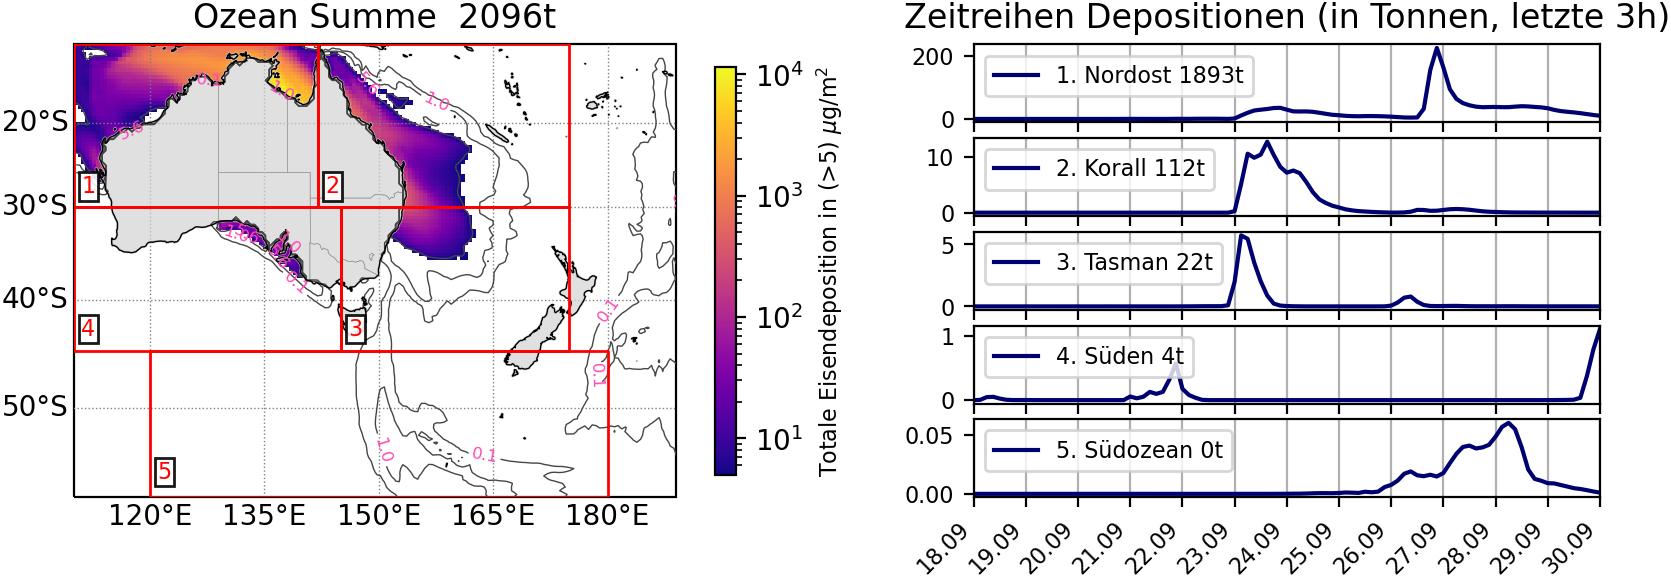
\includegraphics[width=\textwidth]{bilder/total_iron.png}
\caption{Vom WRF-Modell simulierter Eiseneintrag. Die Domäne wird in 5 Sektoren unterteilt: 1. Nordwesten, 2. Korallenmeer, 3. Tasmanisches Meer, 4. Süden, 5. Südozean. Die farbige Kontur gibt die Höhe der des Eintrags für alle Regionen mit einem Eintrag größer als 5 µg/m2 an. Kleinere Einträge sind durch die grauen Konturlinien (1 und 0.1 µg/m2) angezeigt. Rechts sind die jeweiligen Zeitserien der Eiseneinträge für die Regionen dargestellt.} \label{fig:iron_deposition_sections}
\end{figure}
\subsection{Chlorophyll-a Zeitreihen} \label{sec:chla_zeitreihen}
\sloppy 
Abbildung \ref{fig:chla_collage} zeigt anschaulich, dass die Chlorophyll-a-Konzentrationen zwischen Australien und Neuseeland (im Tasmanischen Meer) nach dem Staubsturm (d.h. dem Hauptereignis am 23.09.) ansteigen. Maximale Werte treten am 1. und 2. Oktober auf. Das mutmaßlich aufgrund der Wirbel der Tasmanischen Front \citep{Tilburg.2002} entstandene Muster ist heterogen, Regionen mit hohen Cholorophyll-a-Konzentrationen sind auf entsprechend geformte Bereiche in der turbulent anmutenden Struktur beschränkt, siehe auch Abb. \ref{fig:mld_currents}. Unabhängig von der Entwicklung ist sichtbar, dass die Konzentrationen nördlich von 25-30°S (etwas nördlich der Grenze New South Wales und Queensland) auch im Vergleich zum Südozean per se deutlich geringer sind, mutmaßlich aufgrund des dort geringeren Nährstoffangebots (vgl. Abb. \ref{fig:factors_collage}). Da die Küsten selbst Eisenquellen sein können und/oder je nach Strömungsverhältnissen Regionen mit aufsteigendem nährstoffreichen Wasser bieten können, sind die Konzentrationen dort i.d.R. höher als auf dem offenen Ozean. Speziell das \textit{Great Barrier Reef} an der Nordostküste Queenslands zeigt höhere Chlorophyll-Konzentrationen als in der Umgebung. 
\begin{figure}[htbp]
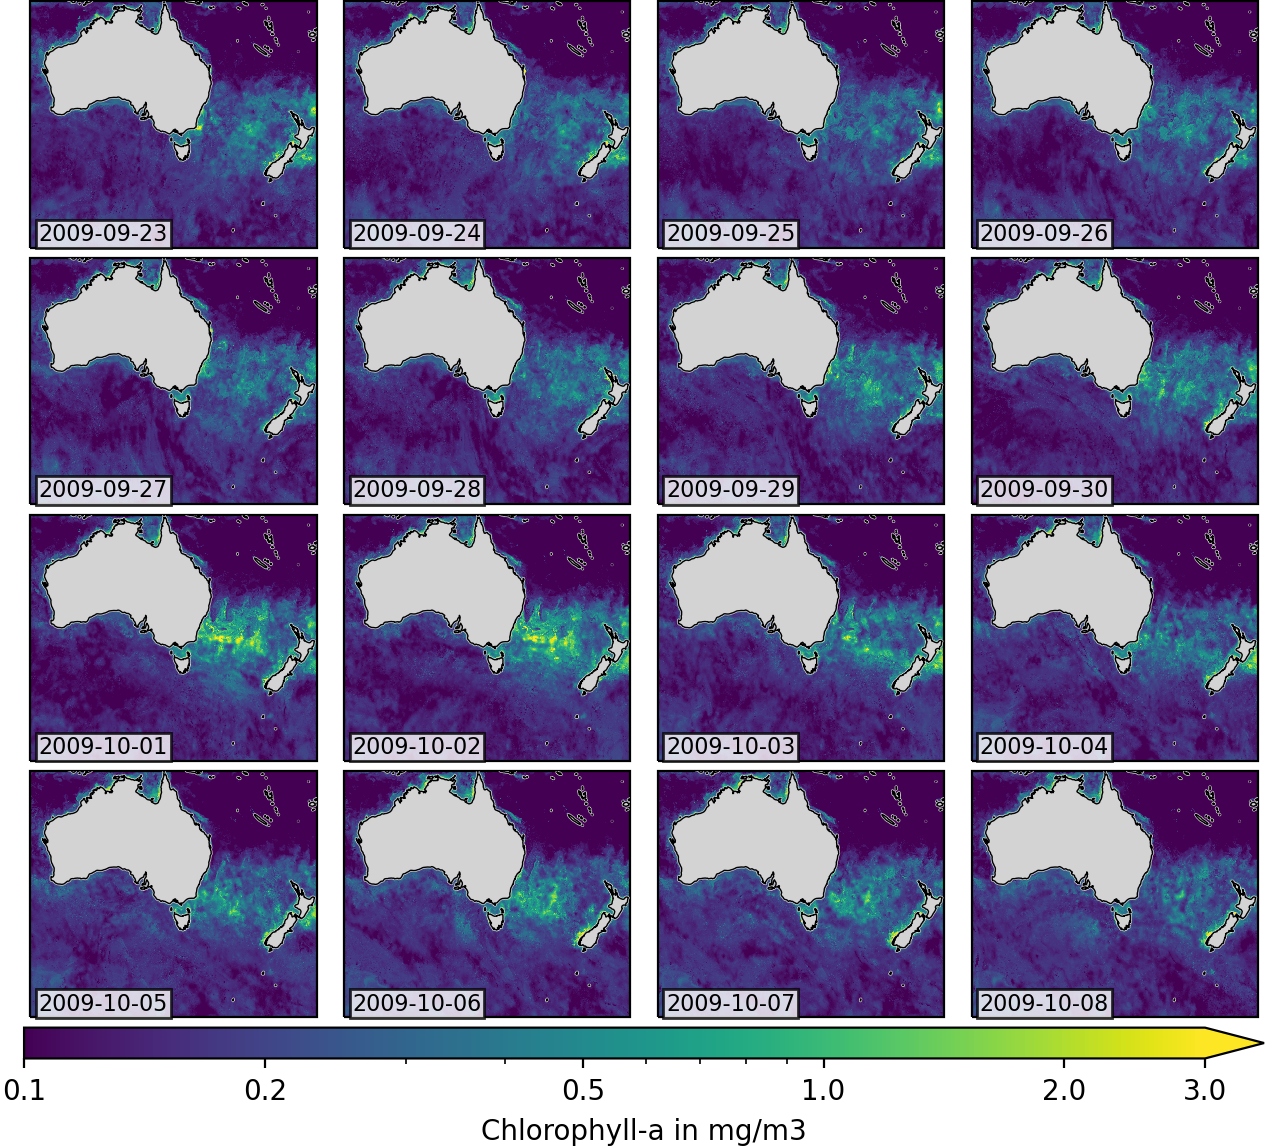
\includegraphics[width=\textwidth]{bilder/chl_collage.png}
\caption{Die Rohdaten für die weitere Analyse: Chlorophyll-a-Konzentrationen für den Zeitraum ab kurz nach dem \textit{Red Dawn Event} bis mehrere Tage danach. Die täglichen Beobachtungsdaten wurden gemäß \cite{Saulquin.2019} interpoliert.} \label{fig:chla_collage}
\end{figure}
Um die Entwicklung des Phytoplanktons genauer zu untersuchen, werden im folgenden Zeitreihen der Chlorophyll-a-Konzentrationen untersucht. Entsprechend Kapitel \ref{sec:timeseries} werden die Mittelwerte für die in Abbildung \ref{fig:iron_deposition_sections} gezeigten 5 verschiedenen Regionen gebildet und deren Zeitreihen für den Zeitraum Juni bis Dezember 2009 präsentiert. Hierbei wurden die Gitterpunkte ausgeschlossen, die direkt an Landflächen grenzen und damit die Küstenzone (von etwa 50km Ausdehnung) repräsentieren. Diese Zonen weisen im Datensatz außerordentlich hohe Werte und Variabilitäten auf, welche mutmaßlich aufgrund von Flussmündungen oder besonderen Wechselwirkungen mit der Küste auftreten. Diese besonderen Effekte können bei der Mittelwertbildung zu Verzerrungen führen. In der rechten Spalte von Abb. \ref{fig:timeseries_full} wird dieselbe Zeitreihe um den jahreszeitlichen Trend bereinigt (gefiltert) und gleichzeitig die Region auf die Gitterpunkte beschränkt, für die das WRF-Modell einen Gesamtstaubeintrag von mehr als 5 µg pro Quadratmeter simuliert. Diese Änderungen in der Darstellung helfen, ein möglicherweise mit den Eiseneinträgen verbundenes Signal zu identifizieren. Ist das Signal der räumlich weiter eingeschränkten Region (in der rechten Spalte) deutlicher als jenes für die gesamte Region (linke Spalte), ist dies sowohl für eine erfolgreiche Simulation der Staub- bzw. Eiseneinträge als auch einen etwaigen Zusammenhang ein positives Indiz. 
\begin{figure}[htbp]
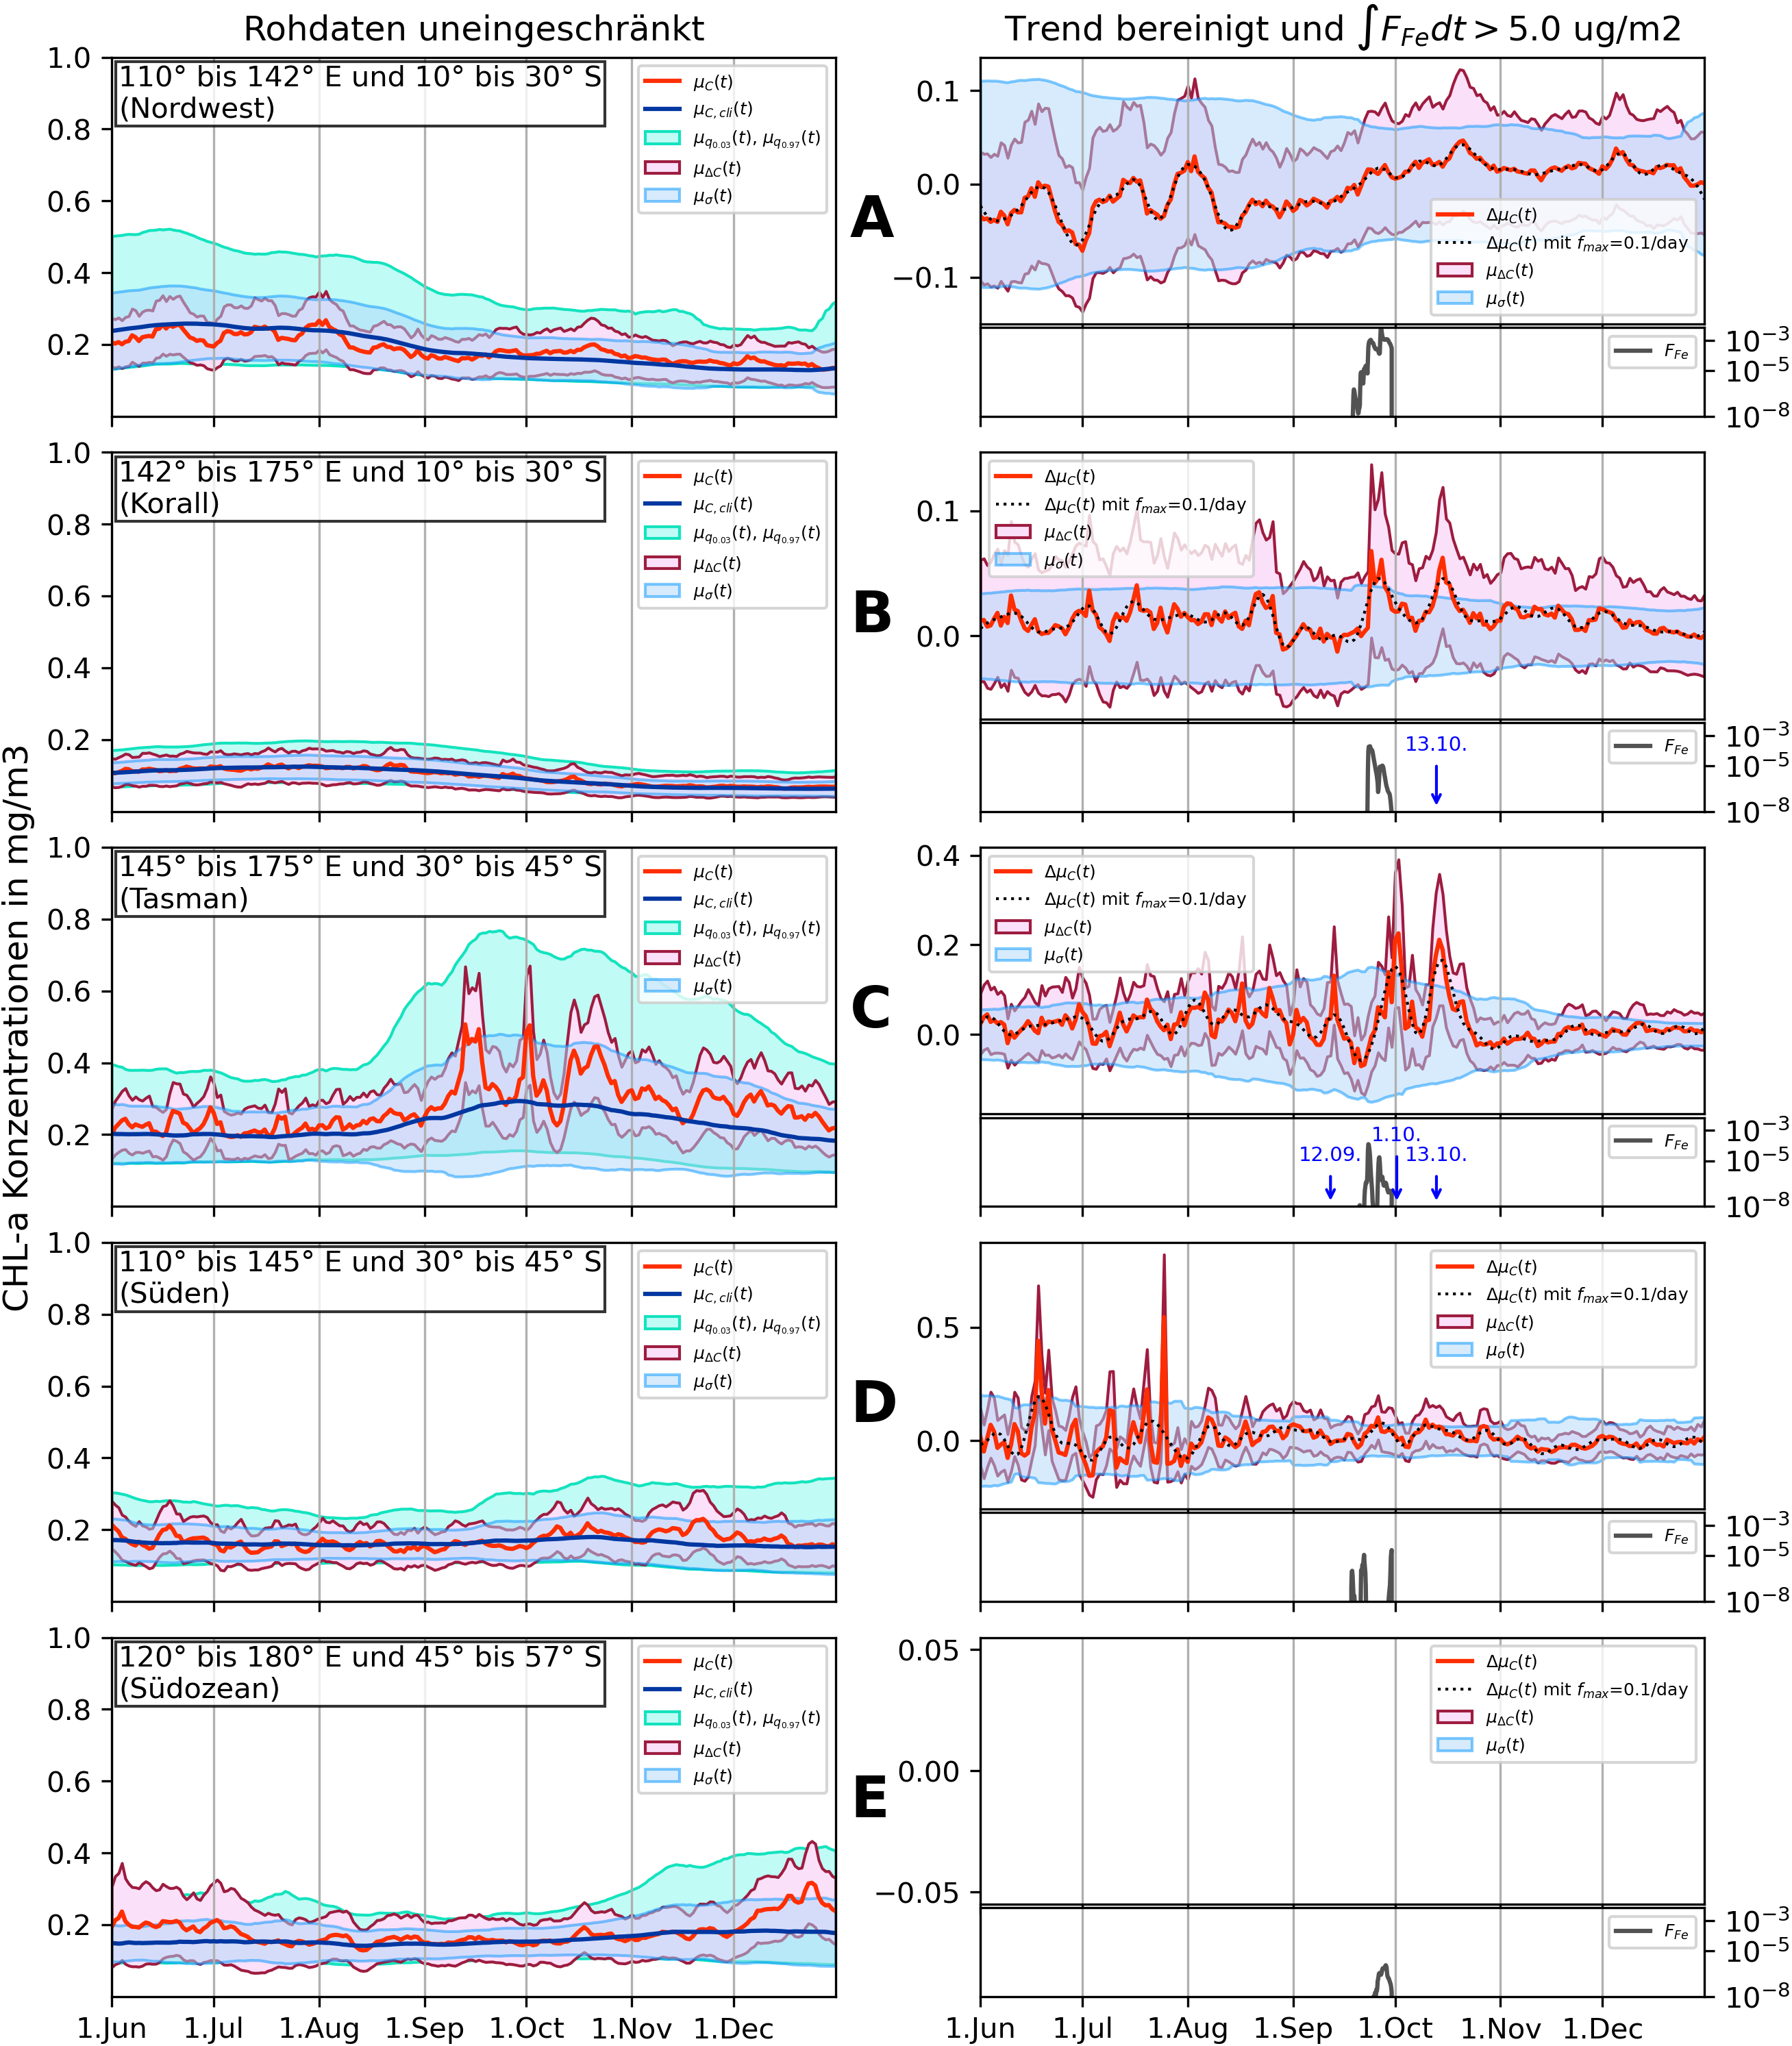
\includegraphics[width=\textwidth]{bilder/timeseries_all.png}
\caption{Zeitreihen vom 1. Juni bis 31. Dezember 2009 der mittleren Chlorophyll-a Konzentrationen für die gemäß Abb. \ref{fig:iron_deposition_sections} unterteilten Gebiete in den jeweiligen Zeilen \textbf{A} bis \textbf{E}. Links ist jeweils die Zeitreihe der Mittelwerte für die komplette Region (ohne Einschränkungen) abgebildet. Rechts daneben in der zweiten Spalte wurden diese \textit{Rohdaten} um die Klima-Mittelwerte korrigiert und das Untersuchungsgebiet auf diejenigen Gitterpunkte beschränkt, für die eine Eisenablagerung von mehr als 5 µg/m2 simuliert wurde. Zusätzlich wurde das Signal mithilfe eines Tiefpassfilters geglättet. Je Zeile rechts unten sind die Zeitreihen der Eiseneinträge für die jeweilige Region dargestellt. Die Pfeile markieren möglichen weiteren Staubeintrag auf Basis der Satellitenbilder in Abb. \ref{fig:duststorms_surrounding} und \ref{fig:satellite_october}. Für die Bezeichnung der Variablen siehe Kapitel \ref{sec:timeseries}}. \label{fig:timeseries_full}
\end{figure}
Anhand Abb. \ref{fig:timeseries_full} ist zu erkennen, dass sich die mittleren Chlorophyll-a-Konzentrationen je nach Region stark unterschieden. So sind bspw. Variabilität und Absolutwerte im Korallenmeer (Abb. \ref{fig:timeseries_full} B) im Vergleich zum sehr viel dynamischeren Tasmanischen Meer (Abb. \ref{fig:timeseries_full} C) sehr gering. Anhand der jeweils auf denselben Wertebereich (0 bis 1 mg/m3) eingeschränkten Beobachtungsdaten in der ersten Spalte sind außer für das Tasmanische Meer kaum nennenswerte Abweichungen von den Klimawerten zu erkennen. Im Tasmanischen Meer (Abb. \ref{fig:timeseries_full} C) sind drei relativ deutliche Signale (positive Abweichungen von den Klimadaten) Mitte September, am 1. Oktober und erneut Mitte Oktober identifizierbar. Allerdings sind in diesem Zeitraum auch die Standardabweichung und das 97 \%-Perzentil der Klimadaten deutlich höher als im restlichen Zeitraum, die Maximalwerte liegen immer noch deutlich unter dem 97 \%-Perzentil. Das lässt darauf schließen, dass zwischenzeitlich erhöhte Chlorophyll-a-Konzentrationen in dieser Region regelmäßig auftreten und möglicherweise mit weiteren Prozessen wie den mit dem Ostaustralstrom assoziierten Wirbeln und einem jahreszeitlichen Gang \citep{Tilburg.2002} verbunden sind. Tatsächlich sieht man bei einer mehrjährigen Betrachtung in Abbildung \ref{fig:long_timeseries_tasman}, dass die Chlorophyll-Konzentrationen im Tasmanischen Meer einem klaren jahreszeitlichen Trend mit regelmäßigen auftretenden Peaks Im Herbst folgen. Dieser Peak fällt für die betrachtete Region im Untersuchungsjahr 2009 am stärksten aus und tritt jedes Jahr ab Mitte September zu einem anderen Zeitpunkt auf.
\begin{figure}[htbp]
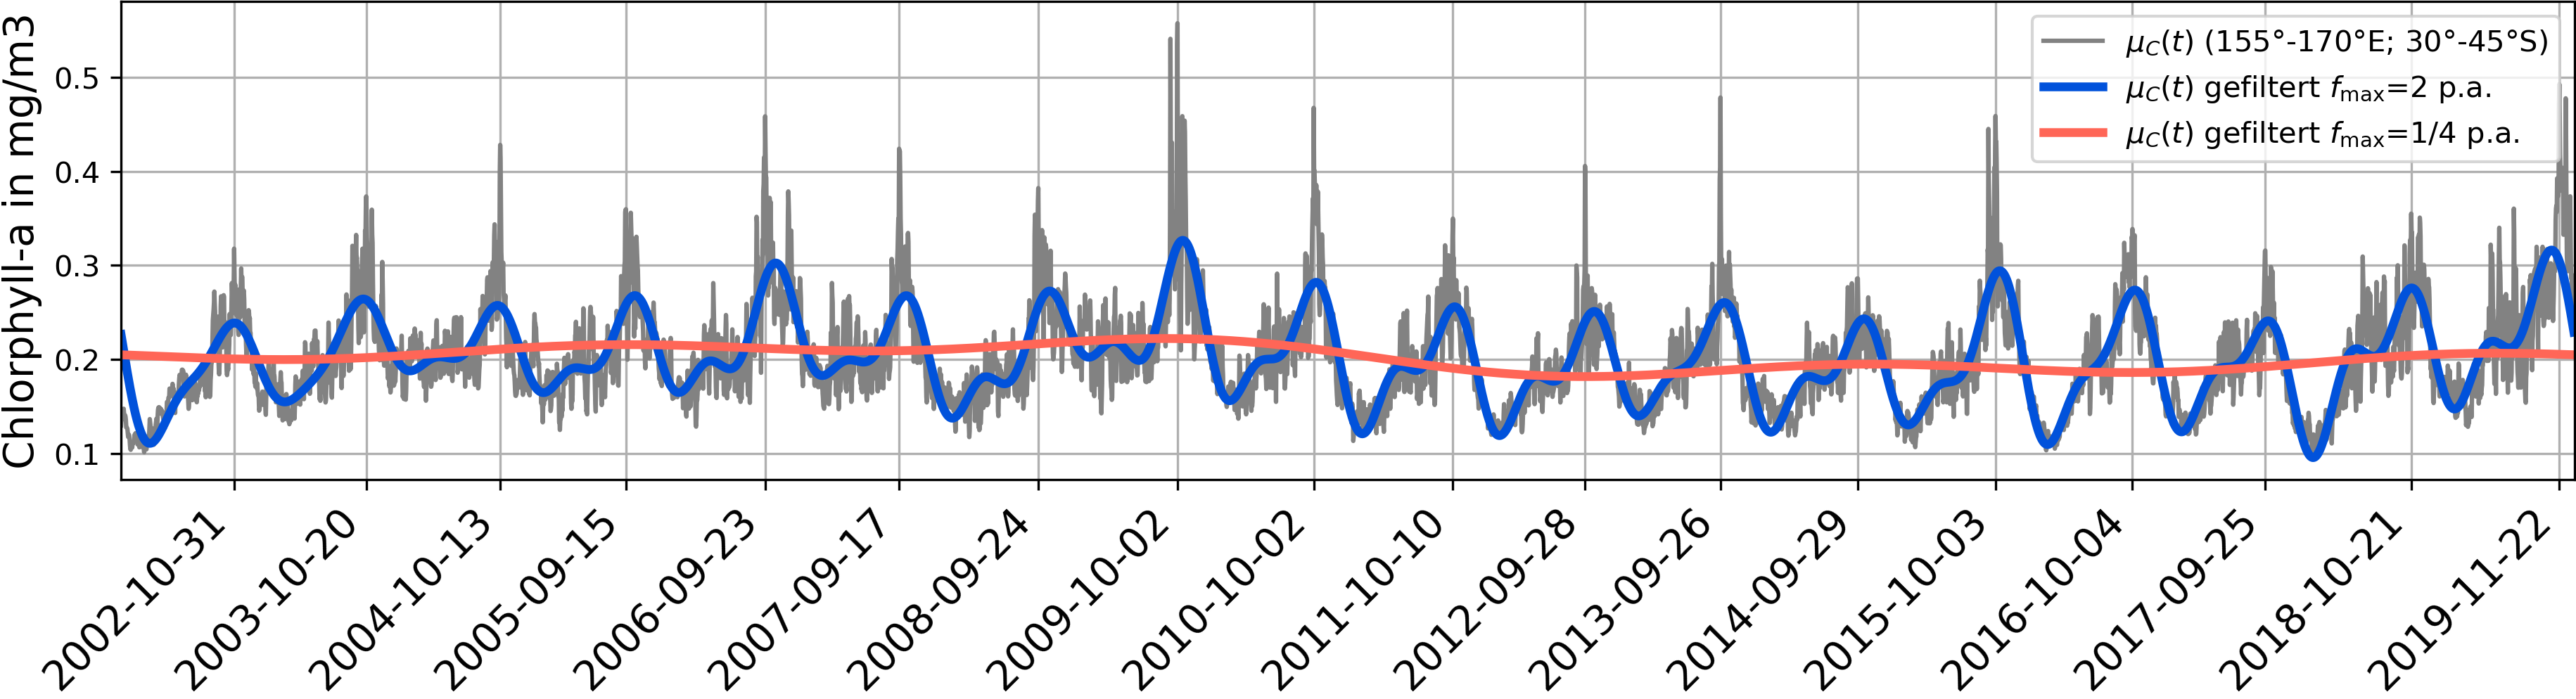
\includegraphics[width=\textwidth]{bilder/long_timeseries_tasman.png}
\caption{Die durchschnittlichen täglichen Chlorophyll-a-Konzentrationen (grau) für einen Teil des Tasmanischen Meeres (155°-170°E und 30°-45°S). Die Zeitreihe wurde zusätzlich auf einen halbjährlichen (blau) und einen vierjährigen (rot) Zyklus Tiefpass-gefiltert. Das auffällige Muster Ende 2019 mit dem vergleichsweise späten Peak ist möglicherweise auf die australischen Waldbrände zu dieser Zeit zurückzuführen \citep{Li.2021}.} \label{fig:long_timeseries_tasman}
\end{figure}
Die Signale aus Mitte September und Mitte Oktober 2009 (Abb. \ref{fig:timeseries_full} C) liegen beide außerhalb des Simulationszeitraums und es wird trotz möglicher Langzeiteffekte \citep{Boyd.2010} nicht angenommen, dass das hier vordergründig untersuchte Staubereignis vom 23. September 2009 noch einen maßgeblichen Einfluss auf die erhöhten Werte Mitte Oktober nimmt. Stattdessen können zu beiden Reaktion anhand von Satellitenbildern ebenfalls Staubereignisse identifiziert werden (siehe Abbildung \ref{fig:duststorms_surrounding}). Es wird angenommen dass diese Ereignisse einen kurzfristigen Einfluss nach wenigen Tagen nehmen können. 
\begin{figure}[htbp]
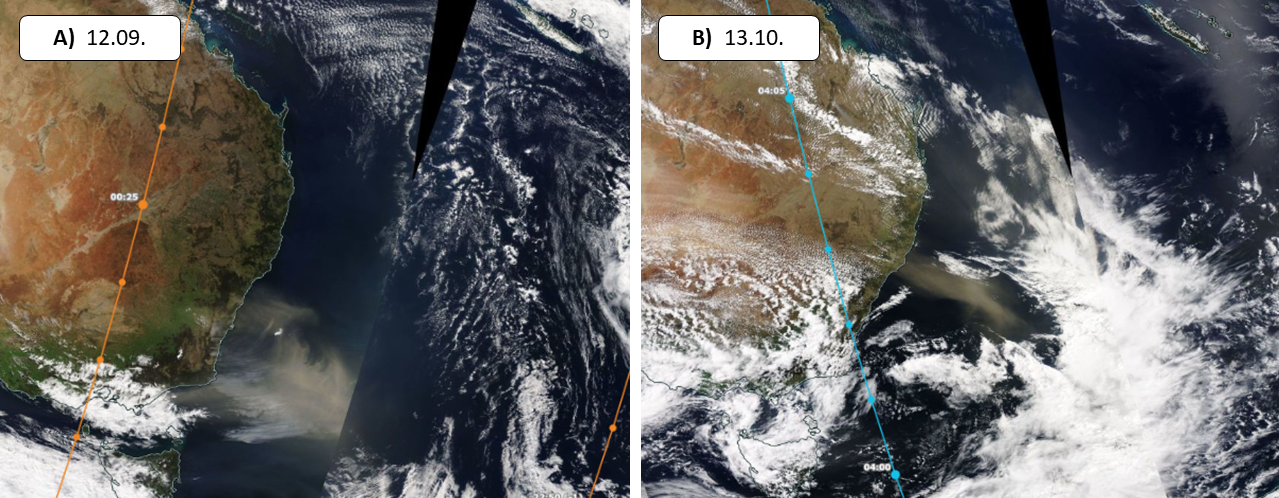
\includegraphics[width=\textwidth]{bilder/duststorms_surround.png}
\caption{Satellitenfotos, aufgenommen mit NASA Worldview. A) Aufnahme TERRA vom 12. September zeigt Staub über dem Tasmanischen Meer. B) Aufnahme AQUA vom 13. Oktober 2009 zeigt ebenfalls Staub über dem Tasmanischen Meer, allerdings etwas nördlicher als in A). } \label{fig:duststorms_surrounding}
\end{figure}
In der rechten Spalte von Abb. \ref{fig:timeseries_full} C ist der jahreszeitliche Trend eliminiert worden. Das Signal aus Mitte September ist hierauf deutlich schwächer ausgeprägt. Dies korrespondiert mit der Beobachtung, dass das möglicherweise zugehörige Staubereignis (siehe Abbildung \ref{fig:duststorms_surrounding} A) weiter südlich aufgetreten ist als der Staubeintrag gemäß der WRF-Simulation. Die erhöhten Werte Mitte Oktober treten hingegen auch in der bereinigten Zeitreihe auf, was aber auch zur räumlichen Ausdehnung entsprechend dem Satellitenbild (Abb. \ref{fig:duststorms_surrounding} B) passt. Von zentraler Bedeutung für diese Analyse ist jedoch mutmaßlich das deutliche Signal in Abb. \ref{fig:timeseries_full} C (rechts) gegen Ende September/Anfang Oktober, welches demnach etwa 5-6 Tage nach dem simulierten Haupt-Eiseneintrag vom 23. September eintritt. Dieses ist insgesamt am höchsten und übertrifft immerhin knapp die mittlere Standardabweichung $\mu_\sigma(t)$ der Klimadaten. Obwohl die Variabilität in dieser Region augenscheinlich ohnehin sehr groß ist, wird angenommen, dass diese erhöhten Chlorophyll-a-Konzentrationen auf das \textit{Red Dawn Event} zurückzuführen sein könnten. Bei \citet{Martin.1988} tritt eine Reaktion des Phytoplanktons nach etwa 4 Tagen auf. Unter realistischen Bedingungen ist eine etwas spätere Reaktion plausibel, da die innerhalb des Staubs auftretenden Eisenpartikel weniger gut löslich sein können \citep{Shao.2011}. Dass dieser zeitliche Zusammenhang zufällig auftritt, erscheint auch hinsichtlich der \textit{benachbarten} Ereignisse Mitte September und Mitte Oktober unwahrscheinlich. \\

Neben dem Tasmanischen Meer sind auf Abbildung \ref{fig:timeseries_full} auch für das Korallenmeer (B, rechts) erhöhte Durchschnittswerte für Ende September/Anfang Oktober und Mitte Oktober auffällig. Die absolute durchschnittliche Anomalie $\Delta \mu_C(t)$ liegt mit knapp +0.1 mg/m3 bei weniger als der Hälfte der durchschnittlichen Anomalie des Tasmanischen Meers mit über 0.2 mg/m3 zur ähnlichen Zeit. Außerdem wird das Maximum etwas früher erreicht. Anhand der Satellitenbilder (Abb. \ref{fig:satellite}) wird deutlich, dass die Staubwolke jedenfalls nahe der Küste einen Großteil des Korallenmeers abgedeckt hat, was unabhängig von der Simulation auf möglichen Staubeintrag hinweist. Auch in den Zeitreihen zu den Regionen im Nordwesten und Süden (\ref{fig:timeseries_full} A und D) sind Tendenzen erhöhter Phytoplankton-Konzentrationen im Oktober erkennbar. Allerdings scheinen hier die Entwicklungen einer tieferen Frequenz zu folgen, es sind keine erheblichen Abweichungen für einzelne Tage erkennbar. Darüber hinaus liegen die Werte stets deutlich innerhalb der Standardabweichung. Für den südlichen Ozean (bzw. südlich des 45°ten Breitengrad) war der Eiseneintrag lt. WRF-Simulation kleiner als 5 µg, weshalb die Zeitreihe in Abbildung \ref{fig:timeseries_full} E leer bleibt. In der (hierfür aber auch  ungeeignet skalierten) Zeitreihe in der ersten Spalte sind keine nennenswerte Signale ableitbar.
\subsection{Räumliche Muster} \label{sec:auswertung_räuml_Muster}
\sloppy
Im vorangegangenen Kapitel \ref{sec:chla_zeitreihen} wird anschaulich gezeigt, dass das Phytoplankton (d.h. die Chlorophyll-a-Konzentrationen) mindestens in den Regionen um das Tasmanische Meer und dem Korallenmeer mit bzw. kurz nach dem Staubeintrag reagiert. In diesem Kapitel sollen die lokalen Veränderungen genauer untersucht werden.
\begin{figure}[htbp]
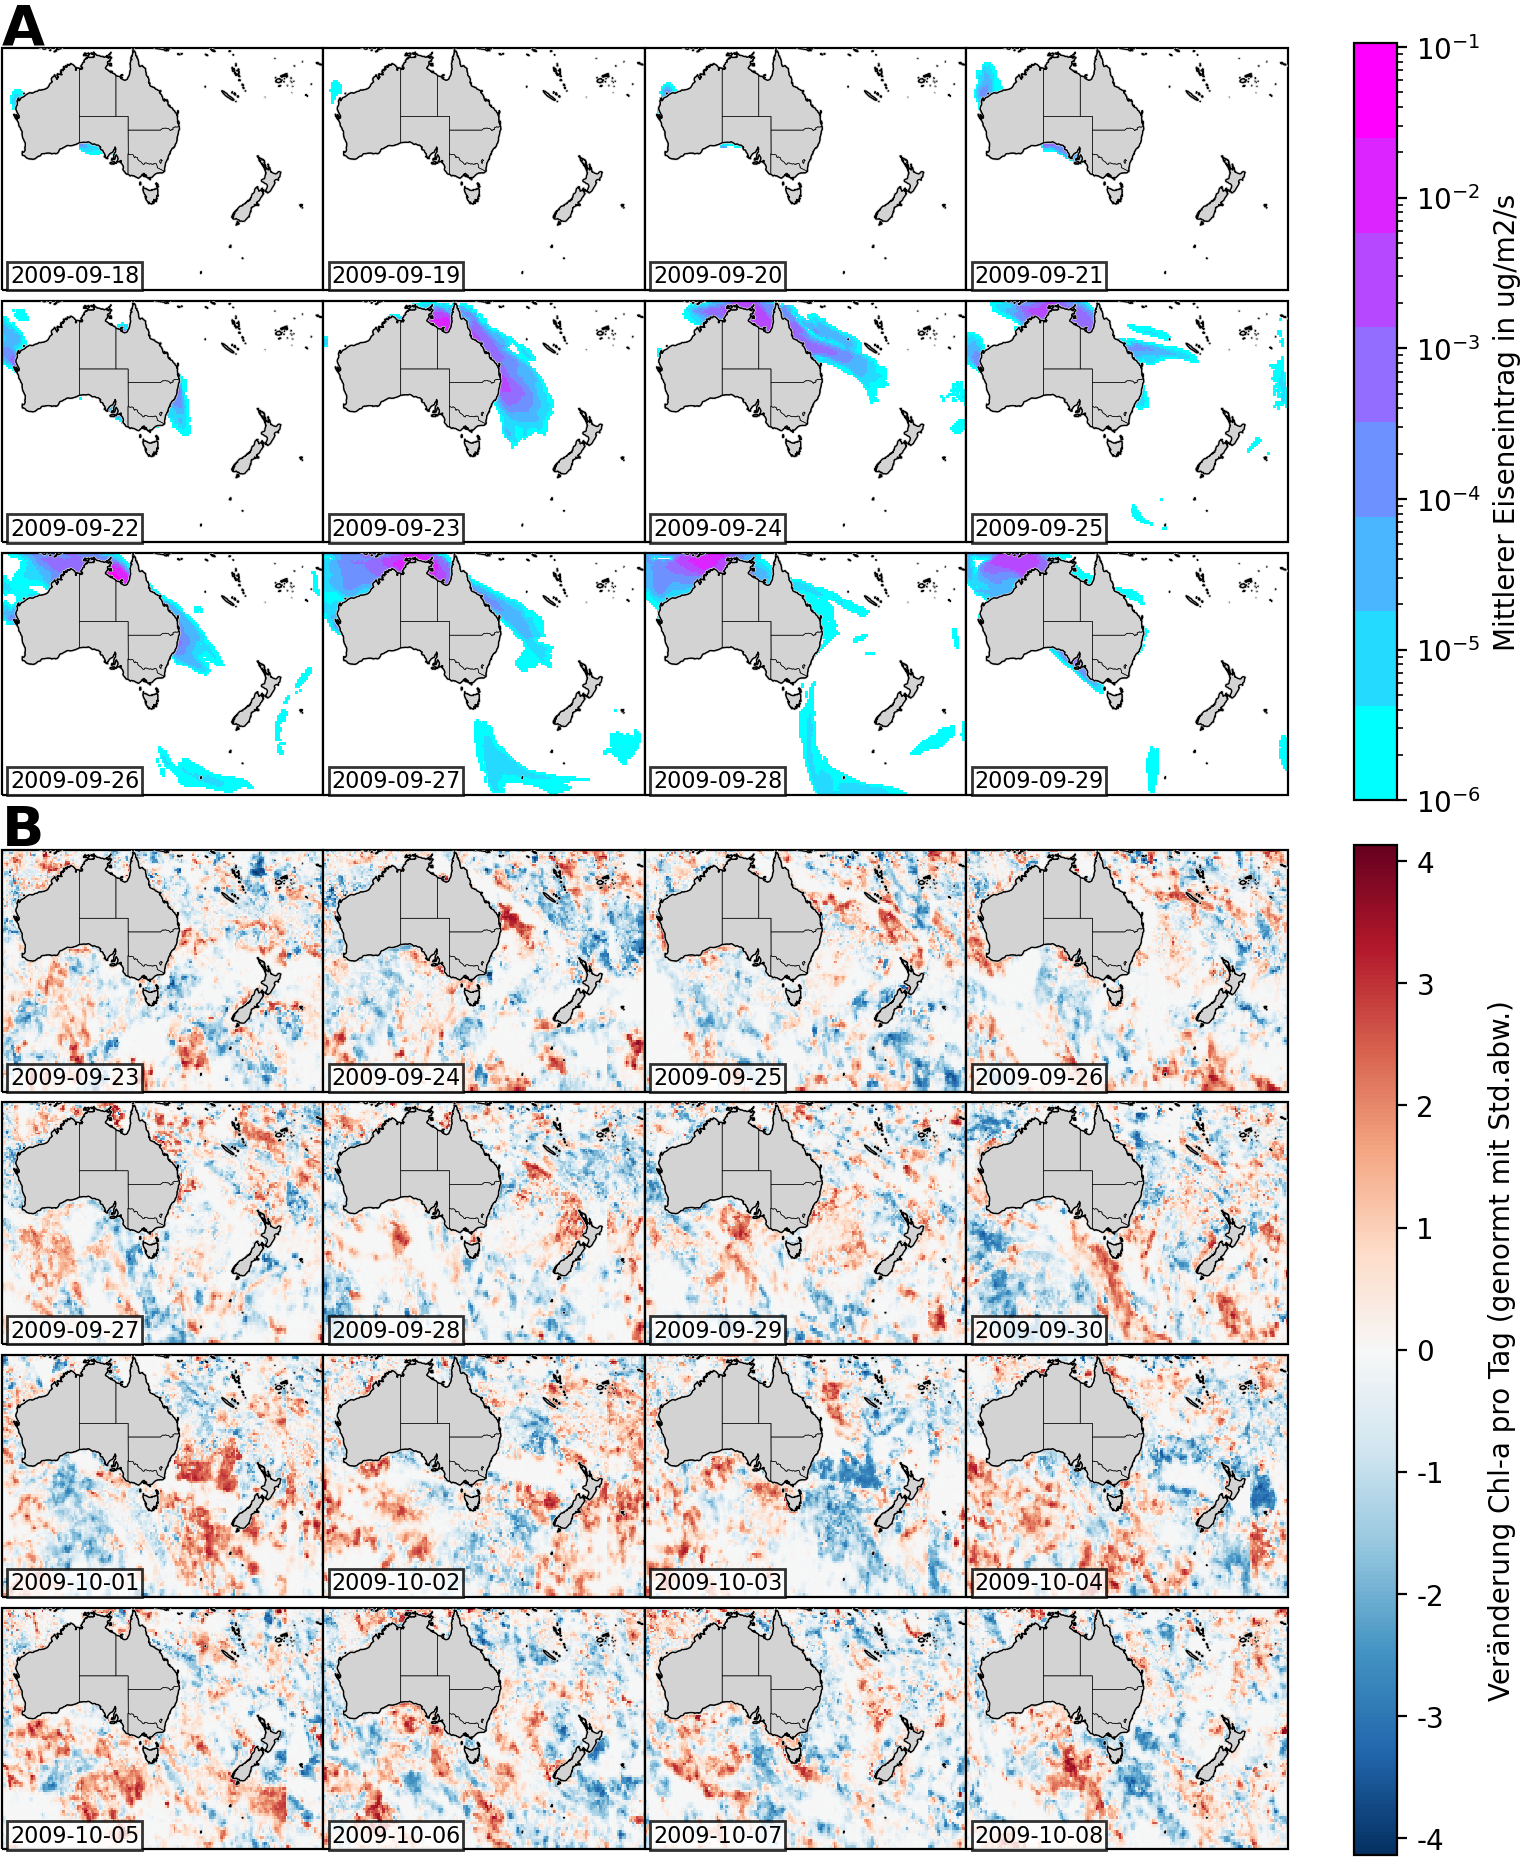
\includegraphics[width=\textwidth]{bilder/snapshot_normalized.png}
\caption{A) Mittlerer täglicher Eiseneintrag für die 12 Tage des Simulationszeitraums. B) Tägliche Änderungen der Chlorophyll-a-Konzentrationen ab dem 22. September. Die Werte wurden für jeden Gitterpunkt mit der zeitlichen Standardabweichung (je Gitterpunkt) normiert, um auch die Muster in Regionen mit geringen Konzentrationen/Abweichungen darzustellen.} \label{fig:snapshot_fedep_chla}
\end{figure}
In Abbildung \ref{fig:snapshot_fedep_chla} können mehrere Muster in den täglichen Eisenablagerungen A) einem ähnlicher Muster positiver Veränderungen bei den Chlorophyll-a-Konzentrationen (\ref{fig:snapshot_fedep_chla} B) zugeordnet werden. Darüber hinaus treten bei den Chlorophyll-a-Konzentrationen weitere Muster auf, die nicht mit Eiseneinträgen erklärt werden können. Dabei ist aber zu berücksichtigen, dass die Entwicklung des Phytoplanktons naturgemäß variabel ist und die Simulation die realen Ablagerungen nicht perfekt wiedergibt (Kapitel \ref{sec:wrf_results}). Die auffälligen Muster sollen hier kurz beschrieben werden. Im Korallenmeer folgt ein Muster positiver Veränderungen der Chlorophyll-a-Konzentrationen dem Muster des Eiseneintrags am Vortag oder desselben Tages. Am 23. September (dem ersten Tag mit nennenswertem Eintrag nördlich des Tasmanischen Meeres (sh. Abb. \ref{fig:iron_deposition_sections}), zeigen sich positive Veränderungen der Konzentrationen im küstennahen Gebiet direkt östlich der Staatengrenze Queensland / New South Wales. Analog zu den Eisen-Niederschlägen streckt sich dieses Muster bis zum 26. September in östliche Richtung und wandert nach Norden ab. Die maximalen Änderungen scheinen am 24. September aufzutreten, der höchste mittlere Eiseneintrag im küstennahen Gebiet erfolgt am 23. September. Eine ähnliche Entwicklung zeigt sich für das  zweite Staubereignis mit zusätzlichem Eintrag beginnend am 26. September. In diesem Fall sind sowohl der simulierte Eiseneintrag und mehr noch die positiven Veränderungen des Chlorophylls im gesamten Verlauf etwas südlicher und das Muster ist stärker unterbrochen. Darüber hinaus ist in \ref{fig:snapshot_fedep_chla} B) am 30. September südlich von Tasmanien eine hauptsächlich Nord-Süd ausgerichtete Struktur positiver Abweichungen zu erkennen, dessen Ausdehnung auffällig ähnlich zu den dortigen (allerdings vergleichsweise schwachen) mittleren Eiseneinträgen am 28. September ist. Die Veränderungen im Nordwesten folgen keinem deutlichen Muster der Staubablagerungen, hier treten maximale Werte vor allem am 22.09., noch vor dem Eintrag auf. An der Küste Südaustraliens wird Eisen lt. WRF-Simulation fast ausschließlich küstennah eingetragen. Dort ist eine Reaktion des Phytoplanktons am 22. September auf den Eintrag vom 21.09. denkbar. \linebreak

Die markantesten und auffälligsten Veränderungen der Chlorophyll-a-Konzentrationen treten allerdings im Tasmanischen Meer auf (diese stechen aufgrund der Normalisierung in Abb. \ref{fig:snapshot_fedep_chla} B weniger deutlich heraus, vgl. stattdessen Abb. \ref{fig:chla_collage}). Am 1. Oktober sind die dortigen Veränderungen großflächig maximal, was auch in der Zeitreihe in Abb. \ref{fig:timeseries_full} C) deutlich wird. Nennenswerter Eintrag findet in dieser Region lt. WRF-Simulation allerdings fast ausschließlich am 23. September statt, mit einem kleinen Zusatzbeitrag im Laufe des 26.09., vgl. Abb. \ref{fig:iron_deposition_sections}. Demnach würde die Hauptreaktion erst 7-8 Tage nach dem Haupteintrag stattfinden, was sich nicht mit den weiter oben beschriebenen vermeintlich grob ähnlichen Mustern deckt, welche etwa 0-2 Tage aufeinander folgen. Allerdings beginnt die Reaktion im Tasmanischen Meer bereits spätestens am 29.09., von diesem Tag an ist die durchschnittlich Entwicklung positiv (vgl. Abb. \ref{fig:timeseries_full} C). Dies entspräche dann einer Reaktionszeit von 5-6 Tagen. Es ist möglich, dass die Oberflächenströmung des Ozeanwassers Einfluss auf diese etwas spätere zeitliche Entwicklung nimmt. Diese wird im Tasmanischen Meer vom aus Nordosten eintreffenden Ostaustralstrom dominiert, welcher dort zum Teil in die sogenannte hauptsächlich ostwärts strömende Tasmanische Front übergeht. Diese Struktur war auch zum Simulationszeitraum im September 2009 ausgeprägt, sh. Abb. \ref{fig:tasman_current}. Aufgrund der Tasmanischen Front würden sowohl das eingetragene Eisen, als auch Phytoplankton ostwärts transportiert. Die Entfernung zwischen der Ostküste Australiens und Neuseeland beträgt grob 1.800 km. Bei einer angenommen mittleren östlichen Strömungsgeschwindigkeit von etwa 0.13 m/s (sh. Abb. \ref{fig:tasman_current}) würde der Transport mithilfe des Oberflächenwassers von Küste zu Küste demnach ca. 160 Tage dauern. Bei Annahme einer maximalen Strömung von ca. 1 m/s (welche nur sehr lokal beschränkt auftritt) würden knapp 21 Tage benötigt. Selbst unter diesen idealisierten Bedingungen (die lt. Reanalyse-Daten des Oberflächenwassers nicht gegeben waren, sh. Abb. \ref{fig:tasman_current} A) wäre ein Transport der aufgrund des Staubsturms erhöhten Eisenkonzentrationen an der Küste von New South Wales und Queensland bis inmitten des Tasmanischen Meeres innerhalb von 8 Tagen eher unrealistisch. Es ist also anzunehmen, dass die hohen Chlorophyll-a-Konzentrationen westlich der Nordinsel Neuseelands am 1. Oktober (sh. Abb. \ref{fig:snapshot_fedep_chla} B) auch aus anderen Prozessen resultieren und/oder ebenso das Phytoplankton nennenswert ostwärts transportiert wurde. Gleichzeitig ist es wahrscheinlich, dass die eingetragenen Staub- und Eisenmengen in dieser Region größer waren, als durch das WRF-Modell abgeschätzt (sh. Kapitel \ref{sec:wrf_results}). Für eine etwaige Reaktion in der Region westlich von Neuseeland ist außerdem anzumerken, dass sowohl die Eisenkonzentrationen (sh. Abbildung \ref{fig:nutrient_iron}) als auch die Vortizität (sh. Abbildung \ref{fig:tasman_current} B) deutlich geringer beobachtet werden als im nordwestlicheren Tasmanischen Meer. Sowohl eine Erhöhung der Durchmischung/Turbulenz (bzw. Vortizität) als auch Hinzufügen des dort mangelhaft verfügbaren Eisens können mutmaßlich leicht verbesserte Bedingungen für das Wachstum von Phytoplankton schaffen.
\begin{figure}[htbp]
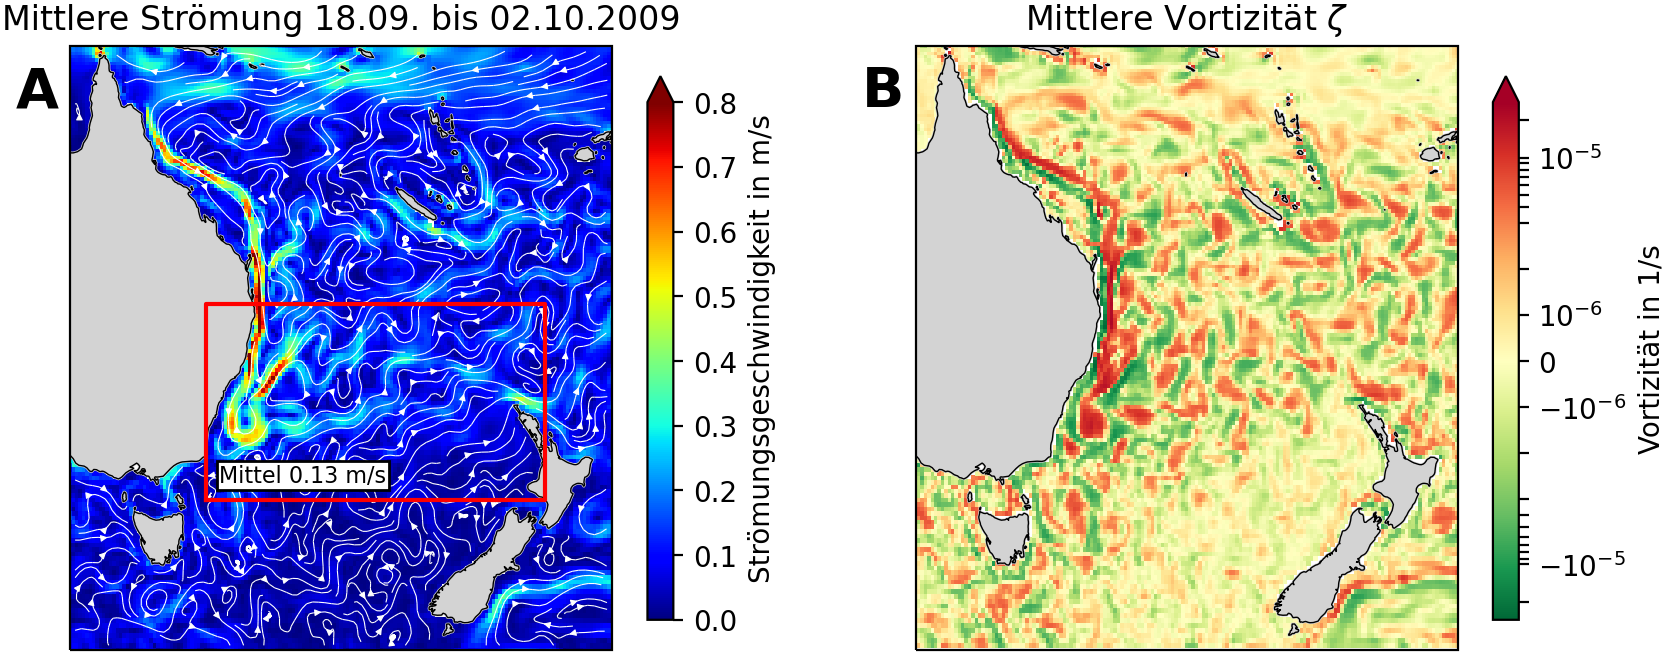
\includegraphics[width=\textwidth]{bilder/currents_mean.png}
\caption{A) Mittlere Strömung für den Untersuchungszeitraum im Tasmanischen Meer mit höheren Geschwindigkeiten innerhalb der Tasmanischen Front (rote Box). Der Teil des Südpazifik-Wirbels trifft aus Nordöstlicher Richtung auf die Küste Queenslands, wird dann südlich abgelenkt und löst sich schließlich wieder Richtung Osten ab und bildet die Tasmanische Front. B) Vortizität in derselben Region. Bereiche mit negativer Vortizität (grün) kennzeichnen zyklonale Wirbel, in denen der Nährstofftransport aus tieferen Schichten gefördert wird. } \label{fig:tasman_current}
\end{figure}
Abbildung \ref{fig:iron_transport}A zeigt die Eisenkonzentrationen im Ozean während und einige Tage nach Ende des Simulationszeitraums, die mit den stark vereinfachten Annahmen zu Transport und Durchmischung (sh. Kapitel \ref{sec:methods_advection}) berechnet wurden. Wie in Abb. \ref{fig:iron_transport} B zu erkennen ist, ändert sich die Verteilung der Konzentrationen durch Advektion nur in geringem Ausmaß. Dies bestätigt die Überschlagsrechnung von zuvor, welche zeigt, dass der Strömungstransport nur über vergleichsweise kurze Distanzen passiert. Allerdings zeigt dies auch, dass die so berechneten Konzentrationen im Osten des Tasmanischen Meeres aufgrund des Eintrags im Osten sukzessive erhöht wurden. Darüber hinaus werden die Konzentrationen kontinuierlich in einem dem Grunde nach gleichen Muster transportiert. Nachdem in den Vortagen des 27.09. Staub hauptsächlich in direkter Nähe der ostaustralischen Küste eingetragen wurde, werden zu den jeweils nächsten dargestellten Zeitpunkten die Konzentrationen in den Regionen östlich des 165. Breitengrads auf Höhe der Tasmanischen Front um bis zu 0.002 nM erhöht, weiter südlich leicht reduziert.
\begin{figure}[htbp]
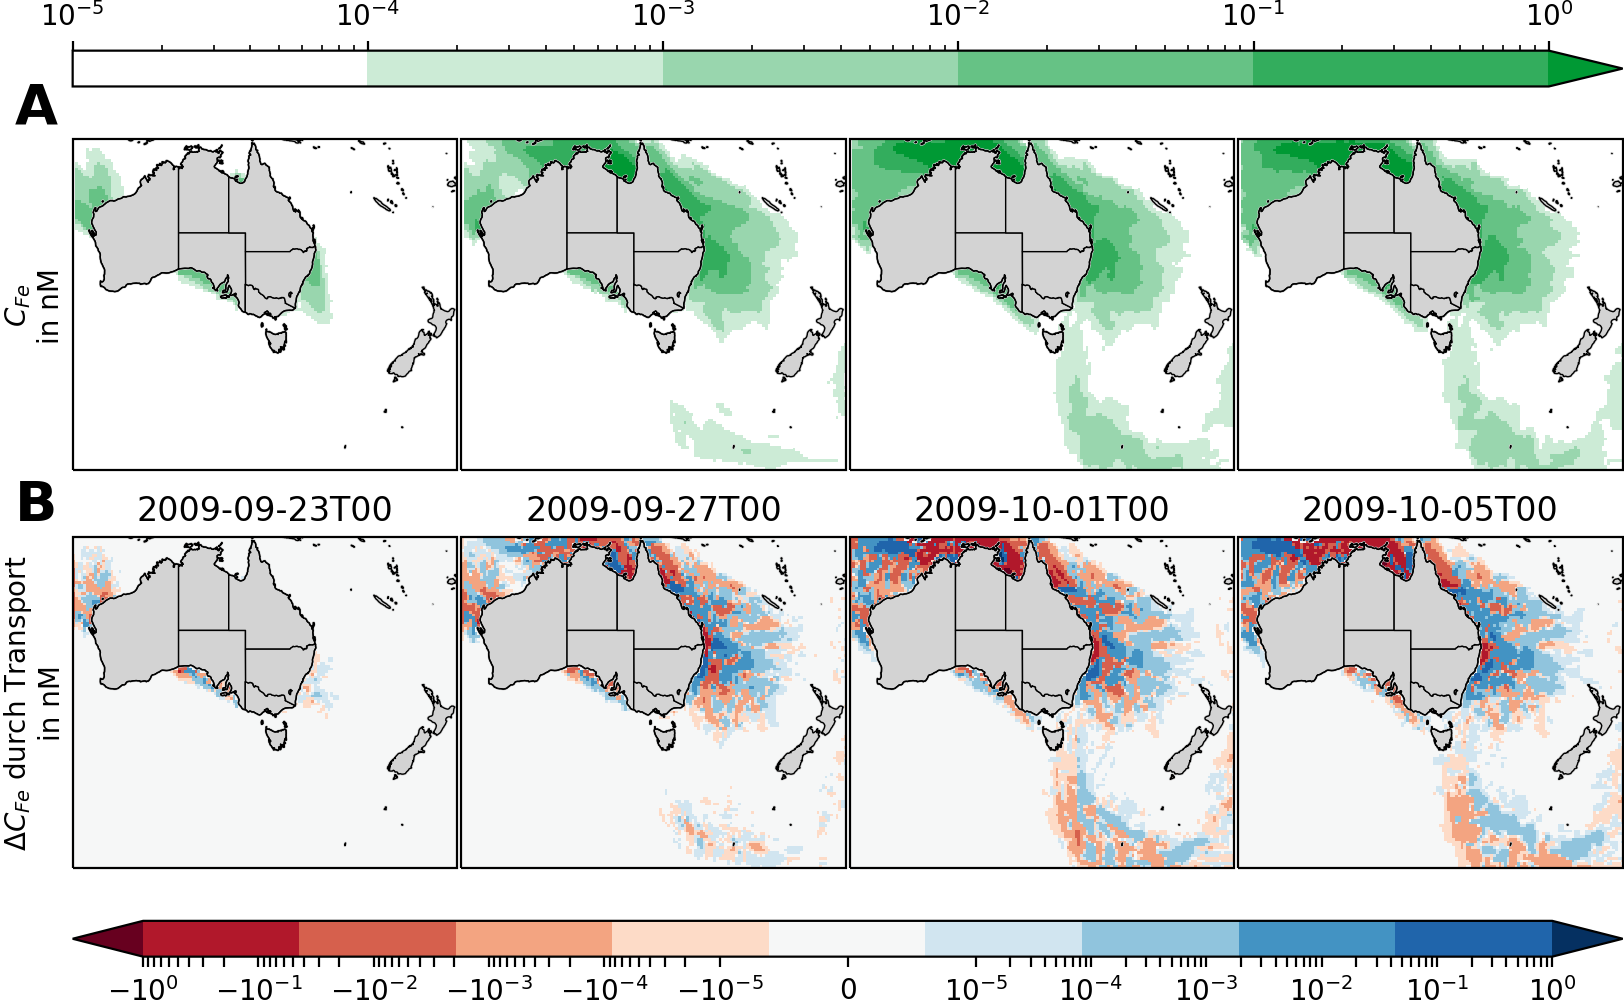
\includegraphics[width=\textwidth]{bilder/iron_transport.png}
\caption{A) Angenommene Eisenkonzentrationen für 4 Zeitpunkte während und nach dem Simulationszeitraum, berechnet gem. Kapitel \ref{sec:methods_advection}. B) Veränderungen der Eisenkonzentrationen aufgrund von Advektion (d.h. exkl. Niederschläge) zum jeweiligen Zeitschritt davor.} \label{fig:iron_transport}
\end{figure}
Angesichts des nur geringen Beitrags scheint es weiterhin fragwürdig, ob die sehr hohen Chlorophyll-Konzentrationen am 1. und 2. Oktober maßgeblich durch den Staubeintrag vom 23. September eingeleitet wurden. Praktisch suggerieren Satellitenaufnahmen des 1. und 2. Oktobers (Abb. \ref{fig:satellite_october}), dass genau zu dieser Zeit in der Region möglicherweise weiterer Staub eingetragen wurde. Dieses potentielle Ereignis wird durch den WRF-Simulationszeitraum leider nicht mehr abdeckt und bisher nicht dokumentiert. Der zugehörige DustWatch Report \citep{Leys.2009b} resümiert, \textit{dass man in der Woche vom 28.09. bis 5. Oktober eine kurze Pause von Staubereignissen} hatte. Die Messstationen wiesen keine erhöhten Werte auf. Nichtsdestotrotz scheint der Zusammenhang vielversprechend (auch angesichts der u.U. sehr schnellen Reaktion des Phytoplanktons von 0-2 Tagen nach Staubeintrag, s.o. bzw. Abbildung \ref{fig:snapshot_fedep_chla}).
\begin{figure}[htbp]
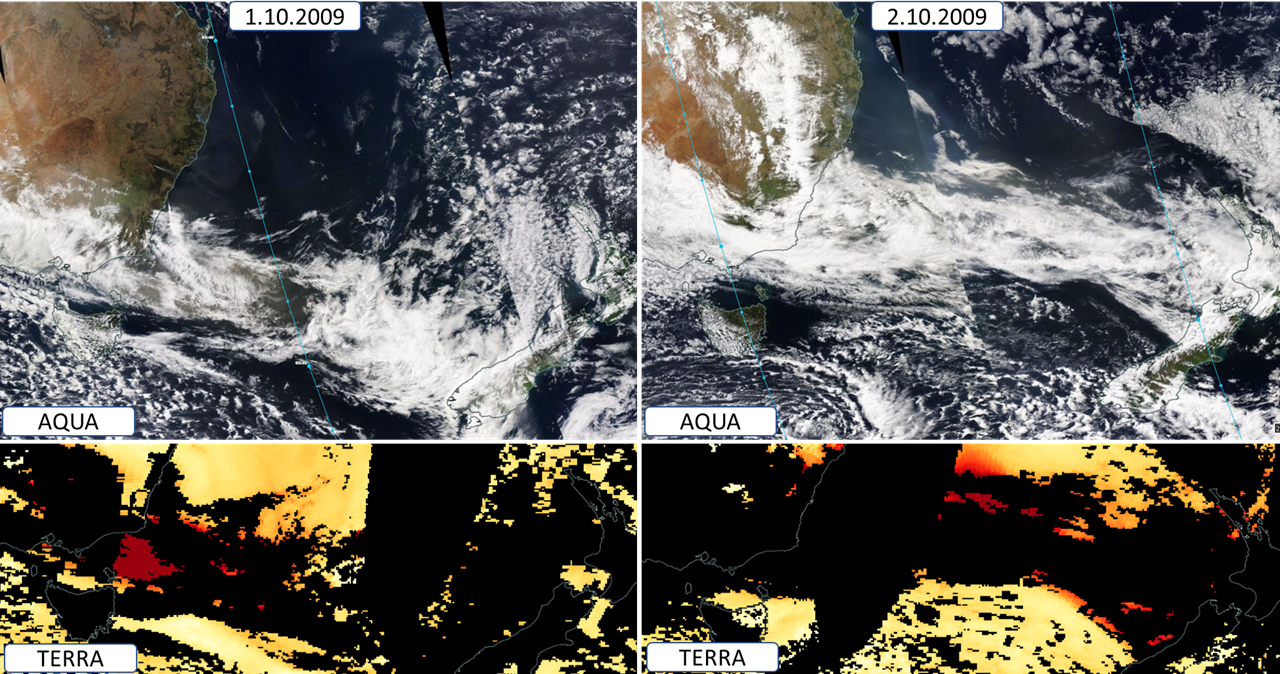
\includegraphics[width=\textwidth]{bilder/satellite_october.png}
\caption{Satellitenaufnahmen (AQUA/TERRA-MODIS) des Tasmanischen Meeres vom 1. und 2. Oktober. Oben: Echtfarben mit deutlicher Signatur im Wolkenband, insbesondere im westlichen Teil. Unten: Erhöhte Aeorosol optische Tiefe (AOD), am 2. Oktober entlang des gesamten Wolkenbandes.} \label{fig:satellite_october}
\end{figure}
Auslöser dieser möglichen Staubemissionen sind gemäß Abbildung \ref{fig:october_weather} wieder starke nördliche/nordwestliche Winde, die mit zwei stark ausgeprägten, direkt aufeinander folgenden Kaltfronten im Zusammenhang stehen. Im westlichen Teil der Staatengrenze Northern Territory / Südaustralien sind die Windgeschwindigkeiten maximal. Etwas weiter östlich von dieser Region sind am 30. September auf der Satellitenaufnahme Terra MODIS (ca. 2 Uhr UTC) in Südaustralien auch Staubbewegungen zu erkennen. Mit dem Durchzug der Fronten gehen erhöhte Niederschläge einher, die die Löslichkeit des darin enthaltenen Eisens weiter erhöhen könnten. 
\begin{figure}[htbp]
	\begin{minipage}[c]{0.3\textwidth}
		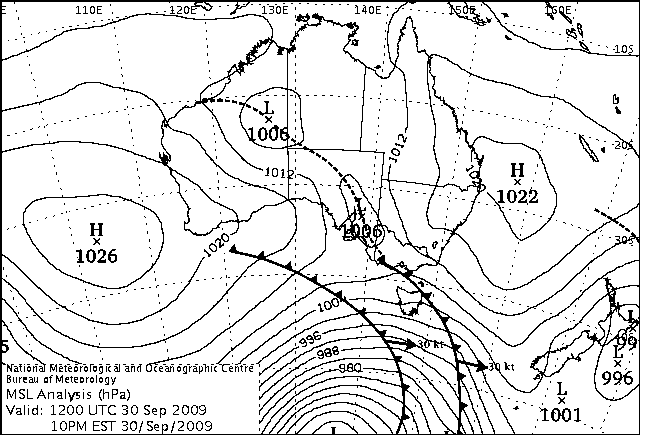
\includegraphics[width=\textwidth]{bilder/20090930T12_msl.png}
	\end{minipage}\hfill
	\begin{minipage}[c]{0.35\textwidth}
		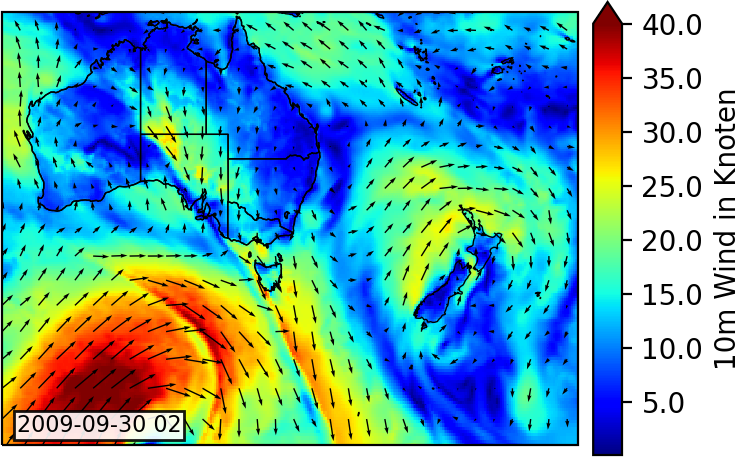
\includegraphics[width=\textwidth]{bilder/wind_october_small.png}
	\end{minipage}\hfill
	\begin{minipage}[c]{0.33\textwidth}
		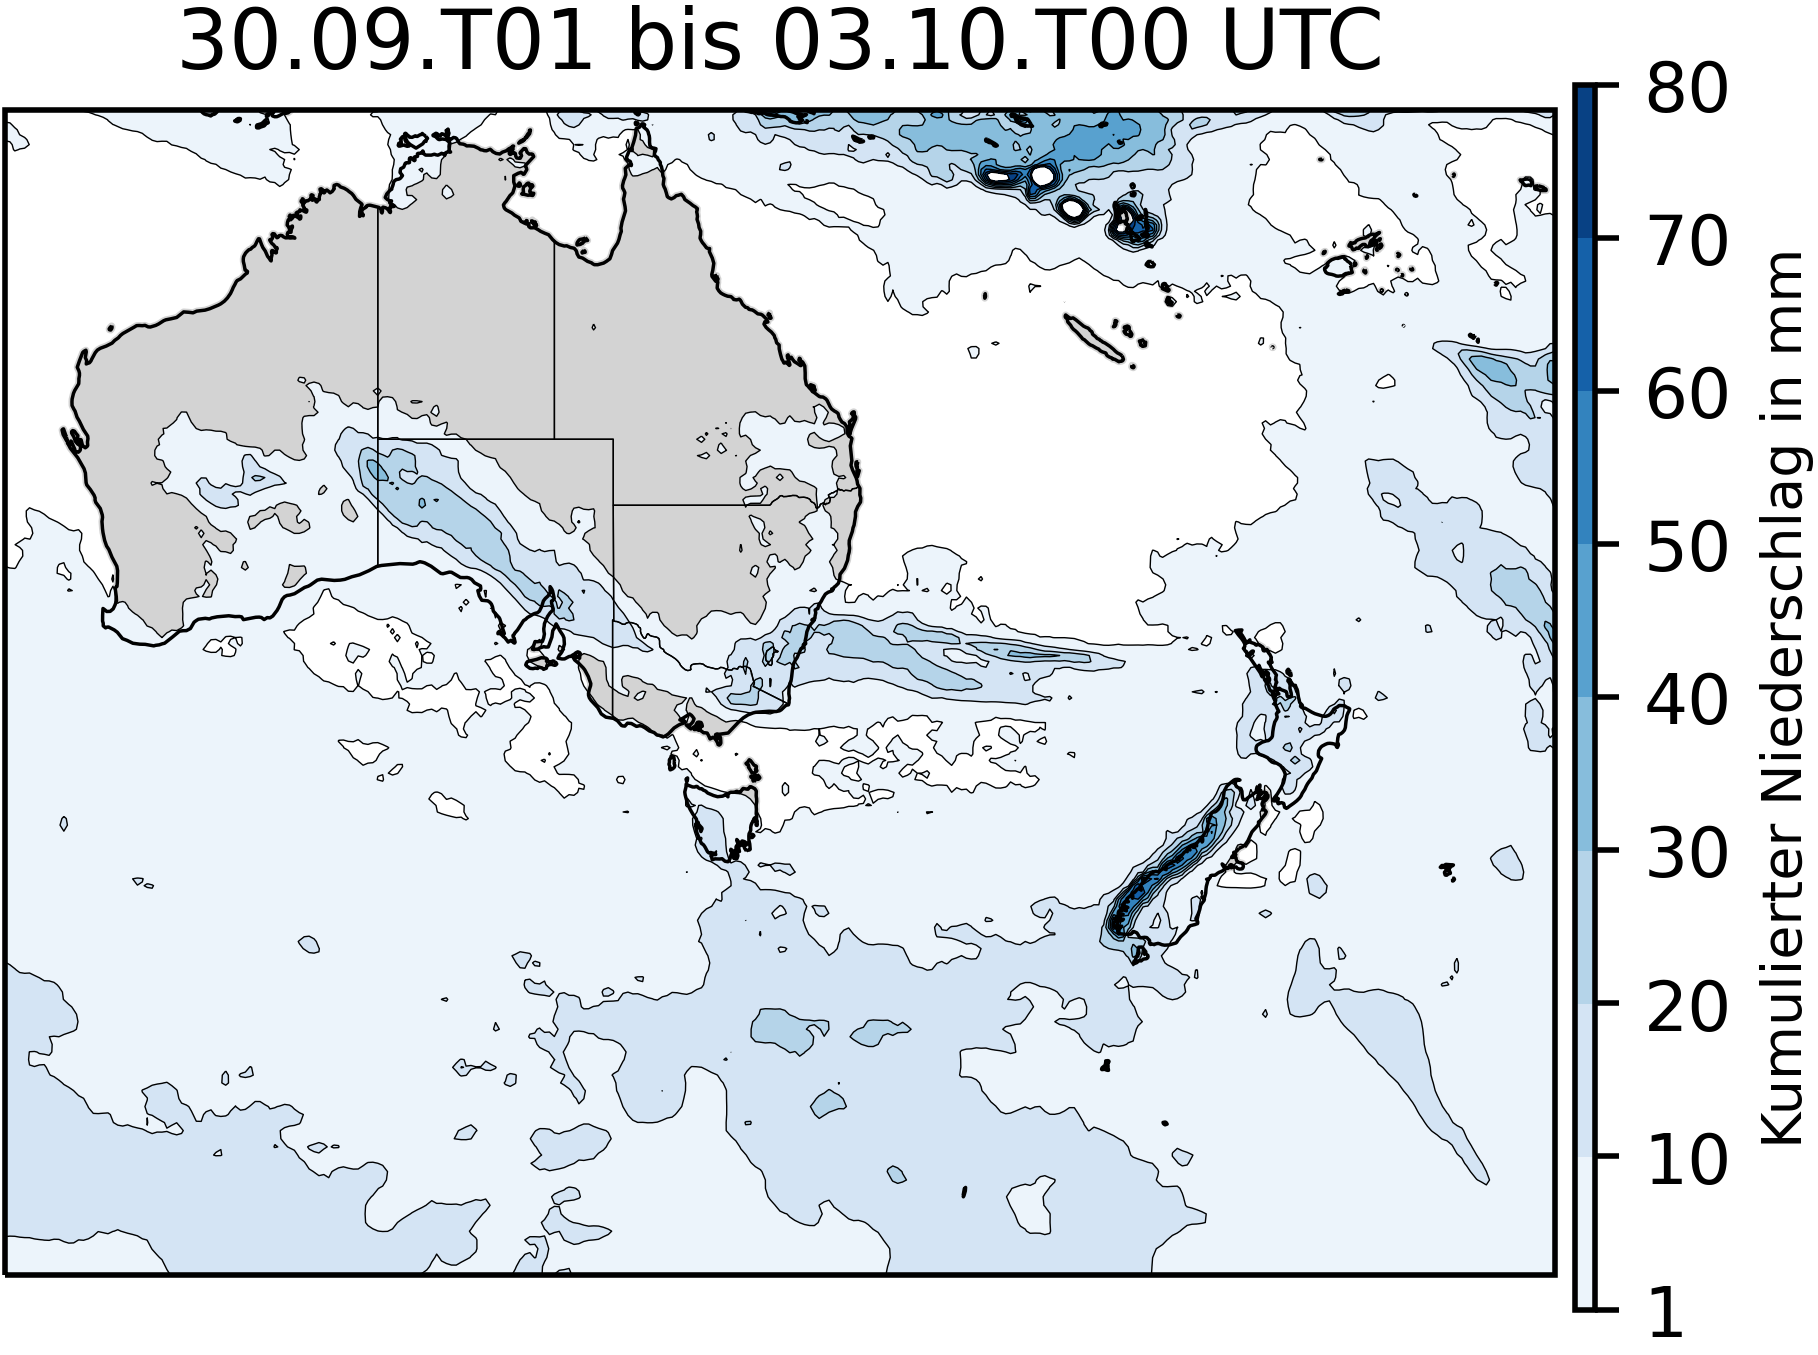
\includegraphics[width=\textwidth]{bilder/rain_october_small.png}
	\end{minipage}\hfill
	\caption{Eine Kurzübersicht zu den Wetterverhältnissen zum möglichen weiteren Staubereignis am 1. und 2. Oktober. Links: Bodendruckanalyse des BoM für 12 Uhr UTC des 30.09. mit der sehr deutlich ausgeprägten doppelten Kaltfront und zwei schwächeren Tiefdruckzonen in West- und Südaustralien. Mitte: Die auf dem Festland maximalen Windgeschwindigkeiten laut Reanalyse-Daten am 30.09. um 2 Uhr UTC. Rechts: Kumulierter Niederschlag für drei Tage ab dem 30.09.2009} \label{fig:october_weather}
\end{figure}
\subsection{Korrelationsanalyse} \label{sec:correlation_analysis}
Unter der Annahme, dass ausschließlich Eiseneintrag (simuliert, näherungsweise linear) zu erhöhtem Phytoplankton-Wachstum führt, sollten die Zeitreihen der Eiseneinträge und Chlorophyll-a-Konzentrationen jedes Gitterpunktes eine hohe Kreuzkorrelation aufweisen. Die besondere Fragestellung ist, um welche \textit{Reaktionszeit} $\tau$ (sh. Kapitel \ref{sec:methods_correlation}) die Zeitreihen der Veränderungen der Chlorophyll-a-Konzentrationen gegenüber denen des Eisenflusses verschoben werden müssen, um eine maximale Ähnlichkeit in der Entwicklung zu erreichen. Diese Reaktionszeit kann dann als die Zeitspanne interpretiert werden, die das Phytoplankton zur Umsetzung des Eisens benötigt. In Ergänzung zu den bisherigen Betrachtungen soll hier zu allen Gitterpunkten eine Korrelationsanalyse ausgewertet werden. Eine mögliche räumliche Verschiebung durch die Strömung nach der Zeit $\tau$ um $\Delta i$, $\Delta j$ wird hierbei entsprechend der jeweiligen Gitterpunktpositionen gemäß Gleichung \ref{eq:position_shift} berücksichtigt. Die für die 5 Regionen (Einteilung analog zu Abb. \ref{fig:timeseries_full}) gemittelten Kreuzkovarianzen (Gl. \ref{eq:covariance}) und Korrelationskoeffizienten (Gl. \ref{eq:corrcoeff}) sind in Abbildung \ref{fig:section_cross_corr} dargestellt.
\begin{figure}[htbp]
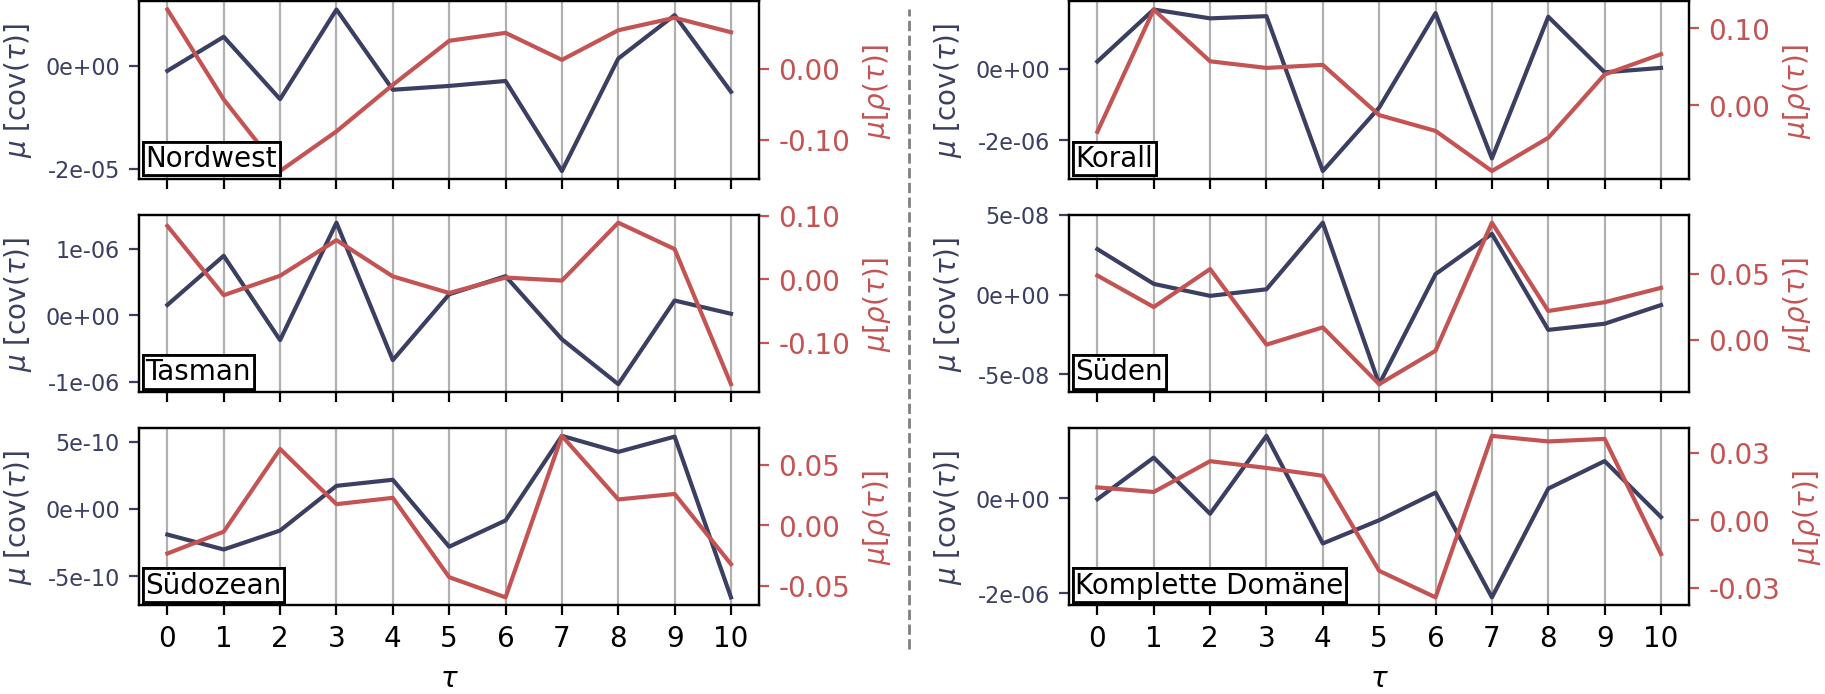
\includegraphics[width=\textwidth]{bilder/section_crosscorr_noadv.png}
\caption{Gemittelte Kreuzkovarianz- und -Korrelationsfunktionen zwischen den Eisenablagerungen und den veränderten Chlorophyll-a-Konzentrationen für die weiter oben definierten Gebiete inkl. räumlicher Verschiebung gem. Strömung.} \label{fig:section_cross_corr}
\end{figure}
Diese stimmen in ihrem Verlauf kaum überein. Es ist keine eindeutige Reaktionszeit $\tau$ erkennbar, nach der die Chlorophyll-a-Konzentrationen in den Gebieten mit Eiseneintrag ansteigen. Es ist allerdings anzumerken, dass die schwache Übereinstimmung der Verläufe von $\mu[\rho(\tau)]$ und $\mu[$cov$(\tau)]$ auch damit zusammenhängt, dass die Gebiete in diesem Fall nicht auf die Regionen mit einer ausreichend (sh. \ref{sec:timeseries}) hohen Eisenkonzentration eingeschränkt wurden, sodass die Variationen in Chlorophyll-Konzentrationen mit kaum bis keinen Eisenkonzentrationen einen hohen Einfluss auf den Mittelwert des normierten Korrelationskoeffizienten $\rho$ nehmen. Trotz der geringen absoluten Höhe der Korrelationskoeffizienten in Abb. \ref{fig:section_cross_corr} sind einige sich wiederholende Merkmale festzuhalten. Die Funktionen nehmen sowohl zu sehr kurzen Zeitverschiebungen von $\tau=$ 0 bis 3 Tagen als auch erneut zu späteren Zeitpunkten nach etwa 7-8 Tagen erhöhte Werte an. Markant sind die hohen Kreuzkovarianzen bei $\tau=3$ Tagen im Nordwesten, im Tasmanischen sowie im Korallenmeer. Da im Nordwesten am meisten Eisen eingetragen wird, wirkt sich dies auch auf die komplette Domäne aus. Ebenfalls fällt auf, dass sich Kovarianz- und Korrelationskoeffizient bei einer Zeitverschiebung von $\tau=8$ Tagen im Tasmanischen Meer erheblich unterscheiden. Obwohl in Abbildung \ref{fig:snapshot_fedep_chla} genau diese Region scheinbar besonders stark reagierte, zeigt sich hier an der Kovarianz, dass der Großteil Eisen im westlichen Teil eingetragen wurde und die Region der maximalen Reaktion nur mit wenigen hohen Absolutwerten abdeckt. Im genormten Korrelationskoeffizient $\rho$ nimmt die absolute Höhe der Werte weniger Einfluss. Auch diese Beobachtung kann darauf hindeuten, dass am 1. und 2. Oktober ein weiteres Staubereignis stattgefunden hat, welches ein zusätzlicher Treiber für die Entwicklung an diesen Tagen ist. Dieses Ereignis scheint allerdings auf den Süden beschränkt und kann demnach nicht die in Abbildung \ref{fig:section_cross_corr} bemerkten höheren Koeffizienten für $\tau=8,9$ im Nordwesten und dem Korallenmeer erklären. Eine weitere Interpretationsmöglichkeit ergibt sich, wenn (dann ohne Berücksichtigung einer räumlichen Verschiebung) zuerst die Mittelwerte (der Eisenablagerungen und Chlorophyll-Veränderungen für die jeweiligen Gebiete) berechnet und anschließend die Kreuz-Kovarianz- und Korrelationsfunktionen zu diesen Mittelwerten dargestellt werden (Abb. \ref{fig:section_means_cross_corr}). In diesem Fall ergeben sich für den Nordwesten, das Tasmanische Meer und den Südozean (in welchen laut Simulation kaum Eisen eingetragen wurde) deutlich für $\tau=8$ die höchsten Korrelationen. Allerdings ist auch hier die Aussagekraft aufgrund des nur kurzen betrachteten Zeitraums von 12 Tagen sehr begrenzt. Der Korrelationskoeffizient überschreitet mit 0.68 im Korallenmeer, 0.59 im Tasmanischen Meer, 0.62 im Südozean nur knapp die für das 95\% Signifikanzniveau erforderliche Schwelle von $\rho(t_{0.975})\approx0.57$ (sh. Kapitel \ref{sec:methods_correlation}). Das Korallenmeer zeigt sogar eine komplett andere Entwicklung mit einem deutlichen Maximum nach einem Tag, bei $\tau=1$. Die Korrelationen zur kompletten Domäne sind in einer ähnlichen Größenordnung, obwohl der Staub bekanntermaßen (sh. Kapitel \ref{sec:wrf_results}) in den verschiedenen Regionen zu verschiedenen Zeiten eingebracht wurde und sich die Chlorophyll-Konzentrationen unterschiedlich entwickelt haben.
\begin{figure}[htbp]
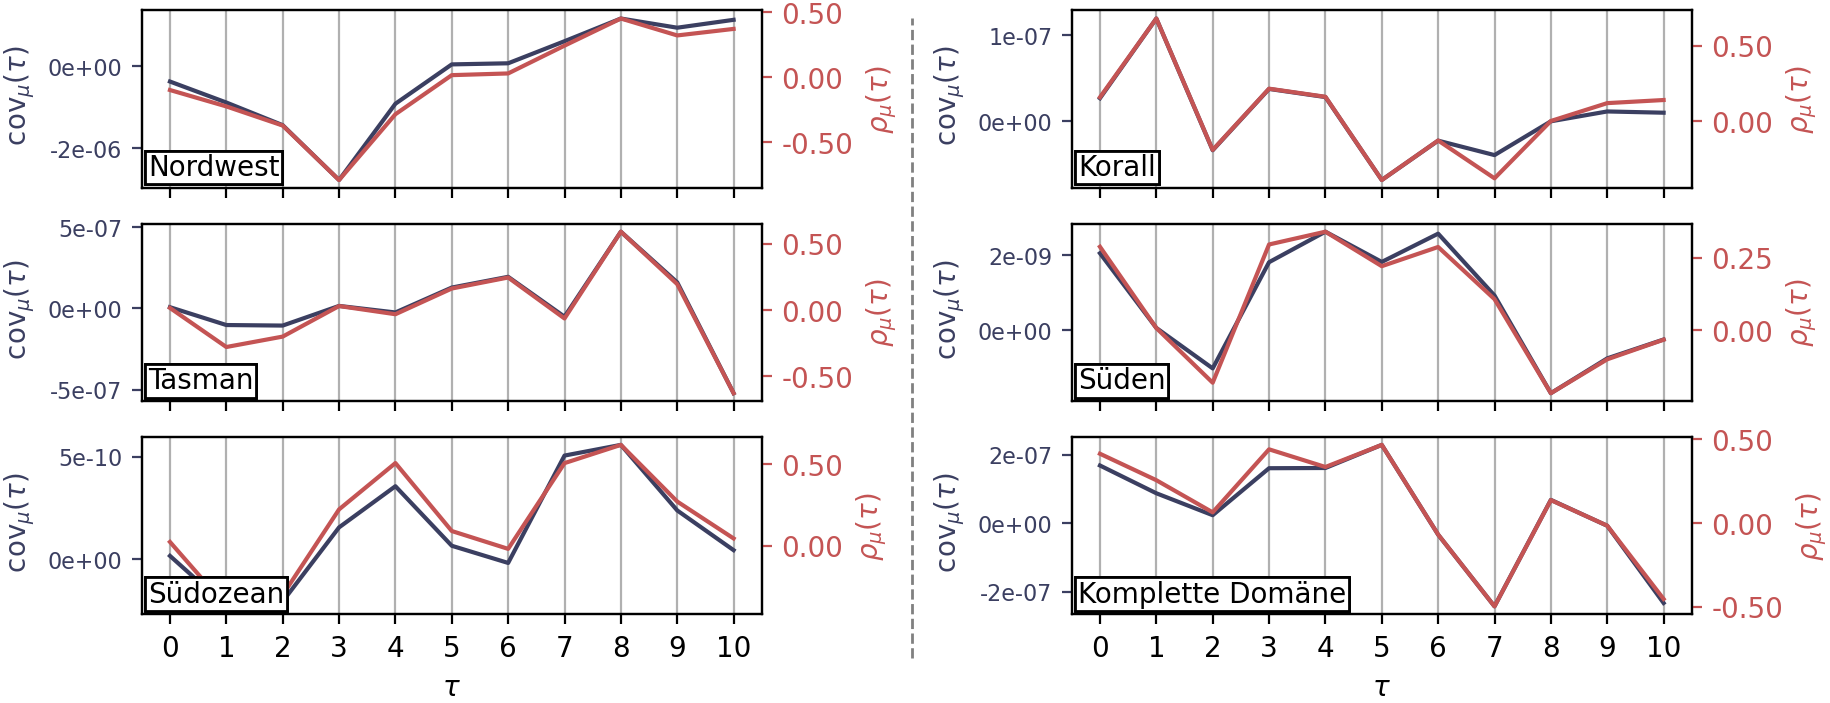
\includegraphics[width=\textwidth]{bilder/section_means_crosscorr_noadv.png}
\caption{Kreuzkovarianz- und -Korrelationsfunktionen für die Mittelwerte der weiter oben definierten Gebiete.} \label{fig:section_means_cross_corr}
\end{figure}
Die räumliche Verteilung der Werte der Koeffizienten je Gitterpunkt ist in Abbildung \ref{fig:correlation_selection} für einige gemäß den Abbildung \ref{fig:section_cross_corr} und \ref{fig:section_means_cross_corr} auffällige Zeitverschiebungen $\tau=$ 1,3,4 und 8 dargestellt. In A) wird die Beobachtung aus Abbildung \ref{fig:section_cross_corr} deutlich, dass die Gitterpunkte zu deutlich unterschiedlichen Zeiten die maximalen Korrelationen aufweisen. Es sind jedoch zwei Gebiete auszumachen, in denen die maximalen Korrelationen über größere Flächen zu derselben Reaktionszeit $\tau$ auftreten. Diese sind ein größerer Teil des Tasmanischen Meeres mit einer Reaktionszeit von 8 Tagen und direkt darüber, der Küstenbereich des östlichen Queenslands mit einer Reaktionszeit von einem Tag. In letzterer Region werden auch im Vergleich zu anderen Regionen insgesamt maximale Korrelationen (Abb. \ref{fig:correlation_selection} B) erreicht. Im Golf von Carpentaria ist eine ähnliche Tendenz zu erkennen. 
\begin{figure}[htbp]
\centering
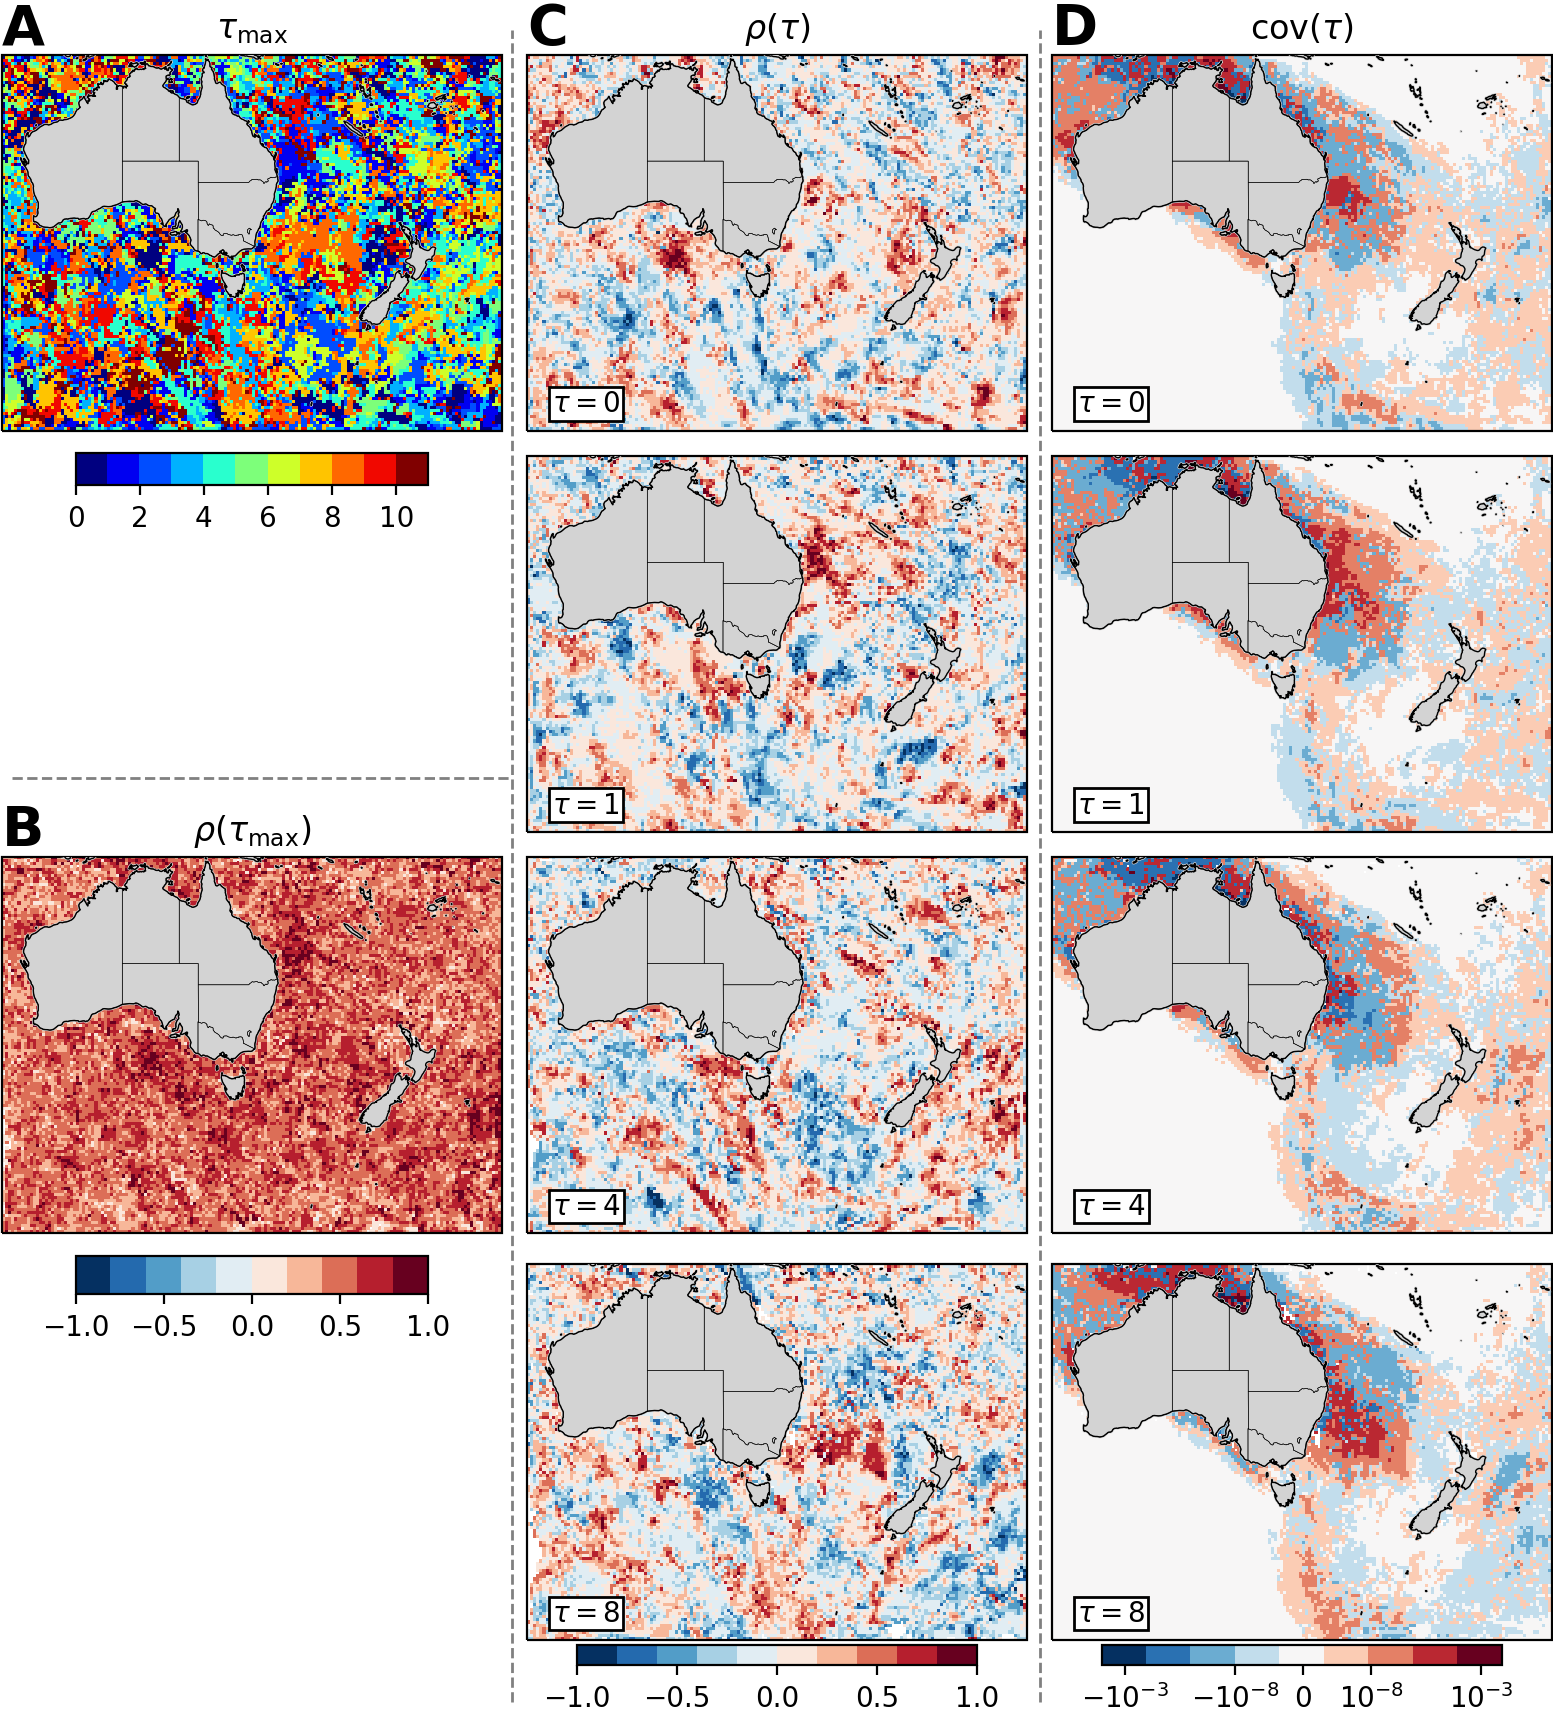
\includegraphics[width=0.8\textwidth]{bilder/correlation_selection.png}
\caption{Kreuz-Kovarianz und -Korrelationskoeffizienten für ausgewählte Zeitverschiebungen $\tau$ inklusive räumlich \textit{maximaler} Verschiebung gemäß Oberflächenströmung. In A) ist das $\tau_\text{max}$ dargestellt, welches für den jeweiligen Gitterpunkt die höchste Korrelation dargestellt. B) Der maximale Korrelationskoeffizient für $\tau_\text{max}$ aus A). C) und D): Kreuz-Korrelation respektive -Varianz für das genannte $\tau$.} \label{fig:correlation_selection}
\end{figure}
\section{Zusammenfassung und Fazit} \label{sec:conclusion}
Der extreme Staubsturm im September 2009 in Australien, besser bekannt als \textit{Red Dawn}, ist ein ausgezeichnetes Untersuchungsobjekt zur Erforschung der Auswirkung von temporären Staubereignissen auf das Phytoplankton im umgebenden Ozean. Staub ist weiterhin ein wichtiger Schlüsselkandidat zur Erklärung der Entwicklung der \cotwo -Konzentrationen in der jüngeren Erdklimageschichte der letzten 800 000 Jahre. Phytoplankton ist als Haupt-\cotwo -Umsetzer ein dominanter Faktor in dieser Entwicklung. Durch die verschiedenen chemischen Eigenschaften in den Ozeanen dieses Planeten haben sich verschiedene Arten ausgebildet, die unterschiedliche Nährstoffbedarfe und Wachstumsraten aufweisen. Die Eisenhypothese von \citet{Martin.1990} ist inzwischen in zahlreichen Experimenten \citep{Boyd.2007} getestet worden und es wurde gezeigt, dass Eisenmangel das Wachstum von Phytoplankton in vielen Regionen tatsächlich limitiert. Gleichzeitig wurde die Hypothese in ihrer Bedeutung aber zugunsten neuerer Kenntnisse in der Ozeandynamik \citep{Tagliabue.2017} teilweise relativiert. Die Ergebnisse dieser Arbeit sollen helfen, den Einfluss der staub-induzierten Eisendüngung transparenter zu machen. Während der südliche Ozean durch den antarktischen Zirkumpolar-Strom und dem damit verbundenen hohen Nährstoffangebot das größte Potential für einen Einfluss auf das globale Klima hat, sind die dortigen eisenspendenden Staubquellen rar gesät. Der australische Kontinent bietet die größten Ressourcen. Dem im Rahmen dieser Arbeit verwendeten WRF-Modell gelingt es, die Staubereignisse im September 2009 zu simulieren, wenngleich die Staubkonzentrationen südlich der Staatengrenze von New South Wales und Queensland vermutlich zu gering repräsentiert sind. Die beobachteten sehr hohen Konzentrationen, die notwendig waren um Sydney in den berühmten rot-orangen Nebel zu hüllen, werden durch die Simulation nicht erreicht. Diese Schwachstelle resultiert möglicherweise aus der Parametrisierung, die dann keine Emissionen in den als Quellen vermuteten \citep{Leys.2011} küstennäheren Weideländern und Bergbaugebieten in New South Wales zulässt. Stattdessen dominiert Channel Country als Hauptquelle mit etwa doppelt so vielen Emissionen wie das südlichere Lake Eyre Becken in Südaustralien. Der größte Teil des emittierten Staubs wird nach kurzer Zeit in Nähe der Quellen wieder eingetragen, ein anderer Großteil verlässt die Domäne im Norden bzw. wird dort eingetragen. Etwa 11\% des in der Domäne eingetragenen Eisens erreicht den Ozean. Nach und während des Simulationszeitraums können tatsächlich markante Veränderungen der Chlorophyll-Konzentrationen festgestellt werden. Es wird davon ausgegangen, dass diese ein Wachstum des Phytoplanktons anzeigen, welches bis dahin aufgrund der Limitierung durch Eisen nicht möglich war. Im Folgenden wird ein einfaches Konzeptmodell formuliert, dass die Entwicklung der Phytoplankton-Bestände erklären soll.
\subsection{Einfaches Konzeptmodell}
Der Staub wird größtenteils in Channel Country und dem südlicheren Lake Eyre Becken emittiert und erreicht nach maximaler Staubbeladung im Laufe des 22.09. zu Beginn des 23.09. die Ostküste Australiens und Sydney. Unmittelbar danach wird ein nennenswerter Teil des eisenhaltigen Staubes in das küstennahe Tasmanische und Korallenmeer eingetragen. In den Teil, der mutmaßlich durch Verfügbarkeit von  Nitraten limitiert ist (vgl. Abb. \ref{fig:factors_collage} A) erfolgt bereits am selben, spätestens am nächsten Tag eine geringe Reaktion des stickstoff-bindenden, dort überwiegenden Picophytoplanktons (u.a. Trichodesmium, \cite{Rubin.2011}) auf das bereits biologisch verfügbare Eisen im Staub. Das per se nährstoff- und chlorophyll- reichere Tasmanische Meer reagiert zu diesem Zeitpunkt noch nicht bzw. verhältnismäßig schwach. Die größtenteils kleinen Staubpartikel werden im Oberflächenwasser aufgenommen, sinken nur langsam ab, sodass das Eisen teilweise gelöst wird. Währenddessen wandert der größte Teil der Staubwolke weiter Richtung Norden/Nordosten, trägt dabei weiterhin Eisenpartikel ein und erzeugt geringfügige Reaktionen des Picophytoplanktons. Ein Teil der Staubwolke gerät aufgrund des Einflusses des Tiefdruckgebietes in eine zyklonale Rotation und wird teilweise, begleitet von Niederschlag, in das Tasmanische Meer eingetragen. Ein weiterer Teil wird durch das Tiefdruckgebiet letztlich nach Süden transportiert. In dieser südlichen Region sind bis auf Eisen sämtliche Nährstoffe (Nitrat, Phosphat, Silikat sh. Abb. \ref{fig:factors_collage}) ausreichend vorhanden, weshalb der dortige Eiseneintrag die Konzentrationen an Kieselalgen ab dem 30.09. in einem ähnlichen Muster (sh. Abb. \ref{fig:snapshot_fedep_chla}) leicht erhöht. Inzwischen wurde aufgrund neuer Emissionen am 26.09. weiteres Eisen in das Tasmanische Meer und Korallenmeer eingetragen, was wieder zu leichten Reaktionen des Picophytoplanktons führt. Das bisher in das Tasmanischen Meer eingetragene Eisen wird weiter gelöst, durch die Tasmanische Front ostwärts transportiert, sodass 5-6 Tage nach dem initialen Haupteintrag die Phytoplankton Konzentrationen am 29.09., gleichzeitig gefördert durch die jahreszeitliche Entwicklung mit einer typischen Frühlingsblüte (sh. Abb. \ref{fig:long_timeseries_tasman}), beginnen zu steigen. Durch ein von Niederschlägen begleitetes zusätzliches Staubereignis am 1. und 2. Oktober (sh. Abb. \ref{fig:satellite_october}, noch zu verifizieren) wird das Nährstoffangebot im südlichen Tasmanischen Meer erneut kurzfristig erhöht. Parallel erhöhen, angetrieben durch ein herannahendes Tiefdruckgebiet (Abb. \ref{fig:october_weather}), südliche Ozeanströmungen die Konzentrationen an Kieselsäure (Abb. \ref{fig:factors_collage} C). Das Zusammenspiel der ursprünglichen - nun gelösten - Einträge durch das Red Dawn Event, des neuen Staubereignisses, der günstigen Meeresströmungen und der Jahreszeit führt schließlich am 1. und 2. Oktober zu einer massiver Phytoplankton-Blüte im Tasmanischen Meer. Gleichzeitig wurde ein Großteil des Staubs in den Nordwesten Australiens eingetragen, in dem keine derartige Reaktion beobachtbar ist, da diese Region zusätzlich durch die Verfügbarkeit von Phosphaten limitiert ist (sh. Abb. \ref{fig:factors_collage} B). \\
\subsection{Ausblick}
Schlussendlich wurde durch diese Arbeit das Ziel erreicht, die Auswirkungen eines Staubsturms auf die Entwicklung des Phytoplanktons zu quantifizieren. Die Resultate könnten nun verwendet werden, die Bedeutung für den Kohlenstofffluss in Richtung Tiefsee abzuschätzen und somit allgemeiner die gesamten Auswirkungen der saisonalen Staubstürme auf den Kohlenstoffkreislauf besser zu verstehen. Für eine möglichst genaue Abschätzung sollte allerdings zunächst das WRF-Modell erneut angepasst werden. Das vermutete weitere Staubereignis vom 1. und 2. Oktober wurde dadurch bisher nicht simuliert. Darüber hinaus ist unklar, ob die Parameter für die Emissionen oder das Emissionsmodell selbst angepasst werden müssen, um alle wichtigen Quellen abzudecken und damit den Eiseneintrag insbesondere im Tasmanischen Mehr bestmöglich abzuschätzen. Auch ohne diese Erweiterungen kann aber bereits konstatiert werden, dass der hier untersuchte extreme Staubsturm einen Einfluss auf das Phytoplankton genommen hat und es sich lohnt, die allgemeine Einwirkung derartiger Staubereignisse auf den Kohlenstoffkreislauf weiter zu untersuchen.

\newpage
\printbibliography
\appendix
%\section{Anhang}

%\addcontentsline{toc}{section}{Abbildungsverzeichnis}
%\listoffigures
%\addcontentsline{toc}{section}{Tabellenverzeichnis}
%\listoftables
\newpage
\section{Verzeichnis der benutzten Hilfsmittel und Danksagung}
Mein besonderer Dank gilt Dr. Sven Ulbrich (Deutscher Wetterdienst), der die für diese Arbeit unverzichtbare WRF-Simulation \glqq produziert\grqq{} und mir weitere wertvolle Tipps gegeben hat. Vielen Dank an Prof. Yaping Shao, Dr. Hendrik Elbern, Dr. Donata Banyte (alle Universität zu Köln) und Prof. Samuel Albani (Università degli Studi di Milano-Bicocca) für den immer interessanten und erfrischenden Austausch und die hervorragende Erreichbarkeit, trotz der Kontaktbeschränkungen. Außerdem möchte ich große Anerkennung an meinen guten Freund Niclas Rieger (CRM Centre for Mathematical Research, Barcelona) für seine didaktischen Fähigkeiten bei unseren spontanen \textit{Python}-Tutorien aussprechen und mich für seine ständige Motivation bedanken. Ein großes Dankeschön geht daneben an Christoph Feder für die spontane Korrekturlesung. Die Darstellungen und Berechnungen im Rahmen dieser Arbeit wurden mit \textit{Python} programmiert. Insbesondere die sehr gut dokumentierten zusätzlichen Module \textit{xarray} und \textit{wrf-python} boten häufig erhebliche Hilfestellungen. Neben der Ausgabedatei aus der WRF-Simulation wurden die Daten des \textit{Copernicus Climate Data Store} (https://cds.climate.copernicus.eu/) und \textit{Copernicus Marine Service} (https://marine.copernicus.eu/) weiterverarbeitet (sh. Tabelle \ref{table:data}). Die Satellitenfotos wurden mit dem Tool \textit{NASA Worldview} (https://worldview.earthdata.nasa.gov/) aufgenommen. Vielen Dank an alle, die den Zugriff auf all die spannenden Daten ermöglicht haben.
\begin{table}[H]
\caption{Übersicht über die verwendeten Daten und deren Quellen} \label{table:data}
\centering
\begin{scriptsize}
\begin{sloppypar}
\begin{tabularx}{\textwidth}{p{2cm} p{2.5cm} X p{2cm}}
		\toprule
			\thead{Variable} & \thead{Anbieter} & \thead{Datensatz} & \thead{Abbildungen} \\
		\toprule
		Chlorophyll-a \newline Konzentrationen & Marine Copernicus \newline Service & OCEANCOLOUR_GLO_CHL_L4_REP_OBSERVATIONS_009_082: dataset-oc-glo-bio-multi-l4-chl_interpolated_4km_daily-rep & \ref{fig:chla}, \ref{fig:chla_collage}, \ref{fig:timeseries_full}, \ref{fig:long_timeseries_tasman}, \ref{fig:snapshot_fedep_chla}, \ref{fig:correlation_selection} \\ \midrule
		Chlorophyll-a \newline (Klimadaten) & Marine Copernicus \newline Service & OCEANCOLOUR_GLO_CHL_L4_REP_OBSERVATIONS_009_082: dataset-oc-glo-bio-multi-l4-chl_4km_daily-climatology & \ref{fig:timeseries_full},\ref{fig:correlation_selection}  \\ \midrule
Strömung \newline Mixed Layer & Marine Copernicus \newline Service & GLOBAL_REANALYSIS_PHY_001_031: global-reanalysis-phy-001-031-grepv2-mnstd-daily & \ref{fig:mld_currents}, \ref{fig:tasman_current} \\ \midrule
Nährstoffe \newline Ozean & Marine Copernicus \newline Service & GLOBAL_REANALYSIS_BIO_001_029: global-reanalysis-bio-001-029-monthly & \ref{fig:factors_collage}, \ref{fig:nutrient_iron}\\ \midrule
Niederschlag \newline Wind & Copern. Climate \newline Data Store & ERA5 hourly data on single levels from 1979 to present (DOI: 10.24381/cds.adbb2d47) & \ref{fig:wind_reddawn}, \ref{fig:rain}, \ref{fig:october_weather}, \ref{fig:factors_collage} \\ \midrule
Eisbohrkerne & National Climatic \newline Data Center &  https://www.ncdc.noaa.gov/data-access/paleoclimatology-data/datasets/ice-core & \ref{fig:icecore}, \ref{fig:co2iron} \\ \midrule
Phytoplankton & Marine Copernicus Service & OCEANCOLOUR_GLO_CHL_L4_REP_OBSERVATIONS_009_082: dataset-oc-glo-bio-multi-l4-pft_4km_monthly-rep & \ref{fig:dominant_diatom_pico} \\ 
\bottomrule
\end{tabularx}
\end{sloppypar}
\end{scriptsize}
\end{table}
Hiermit versichere ich an Eides statt, dass ich die vorliegende Arbeit selbstständig und ohne die Benutzung anderer als der angegebenen  Hilfsmittel angefertigt habe. Alle Stellen, die wörtlich oder sinngemäß  aus veröffentlichten und nicht veröffentlichten Schriften entnommen wurden,  sind als solche kenntlich gemacht. Die Arbeit ist in gleicher oder  ähnlicher Form oder  auszugsweise im Rahmen einer anderen Prüfung noch nicht vorgelegt worden. Ich versichere, dass die eingereichte  elektronische Fassung der eingereichten Druckfassung vollständig  entspricht.
\end{document}
